\documentclass[11pt,a4paper,oneside]{book}
\usepackage[margin=21mm,headheight=16pt]{geometry}
\usepackage{fontspec}
\setmainfont{Noto Sans}
\newfontfamily\displayfont{EB Garamond}
\usepackage{xcolor,graphicx,enumitem,tabularx,booktabs,titlesec,fancyhdr,microtype}
\usepackage[most]{tcolorbox}
\usepackage{pdfpages}
\usepackage{hyperref}
\definecolor{paper}{HTML}{FFFDFA}
\definecolor{ink}{HTML}{2A354B}
\definecolor{navy}{HTML}{08142C}
\definecolor{blue}{HTML}{274B75}
\definecolor{rule}{HTML}{E1DACA}
\pagecolor{paper}\color{ink}
\hypersetup{colorlinks=true,urlcolor=blue,linkcolor=blue,pdftitle={English C — Course Lessons},pdfauthor={}}
\setlength{\parindent}{0pt}
\setlength{\parskip}{.55em}
\setlength{\emergencystretch}{2em}
\linespread{1.12}
\setlist{leftmargin=*,itemsep=.35em,topsep=.4em,parsep=0pt}
\setlist[enumerate]{label=\textcolor{blue}{\arabic*.}}
\titleformat{\section}{\displayfont\Large\color{navy}}{}{0pt}{}
\titlespacing*{\section}{0pt}{1.2em}{.5em}
\titleformat{\subsection}{\bfseries\color{blue}}{}{0pt}{}
\titlespacing*{\subsection}{0pt}{.9em}{.3em}
\newcommand{\tasktitle}[1]{{\color{blue}\bfseries #1}\par\smallskip}
\newtcolorbox{taskbox}{enhanced,colback=paper,colframe=paper,boxrule=0pt,left=3mm,right=1mm,top=1mm,bottom=1mm,before skip=5pt,after skip=8pt}
\newtcolorbox{quotebox}{enhanced,breakable,colback=paper,colframe=rule,boxrule=0pt,borderline west={2pt}{0pt}{rule},fontupper=\displayfont\large,left=5mm}
\pagestyle{fancy}\fancyhf{}
\fancyhead[L]{\small\color{blue}Course lessons}
\fancyhead[R]{\small English C}
\fancyfoot[L]{\footnotesize\nouppercase{\leftmark}}
\fancyfoot[R]{\small\thepage}
\renewcommand{\headrulewidth}{0pt}
\makeatletter
\renewcommand{\@pnumwidth}{2.2em}
\renewcommand{\@tocrmarg}{3em}
\makeatother
\setcounter{tocdepth}{1}
\begin{document}
\begin{titlepage}
\vspace*{30mm}
{\color{blue}\large COURSE LESSONS\par}
\vspace{10mm}
{\displayfont\color{navy}\fontsize{48}{52}\selectfont English C\par}
\vspace{12mm}
{\Large Identity\par Voice\par The Future Is Written\par}
\vfill
{\color{blue}24 lessons · August–November 2026\par}
\end{titlepage}
\tableofcontents

\clearpage\phantomsection\addcontentsline{toc}{chapter}{1. Identity}\markboth{Identity}{}\thispagestyle{empty}
\fancyhead[L]{\small\color{blue}Identity}
\vspace*{12mm}
{\color{blue}\large CHAPTER 1\par}\vspace{8mm}
{\displayfont\color{navy}\fontsize{43}{47}\selectfont Identity\par}\vspace{12mm}
\begin{center}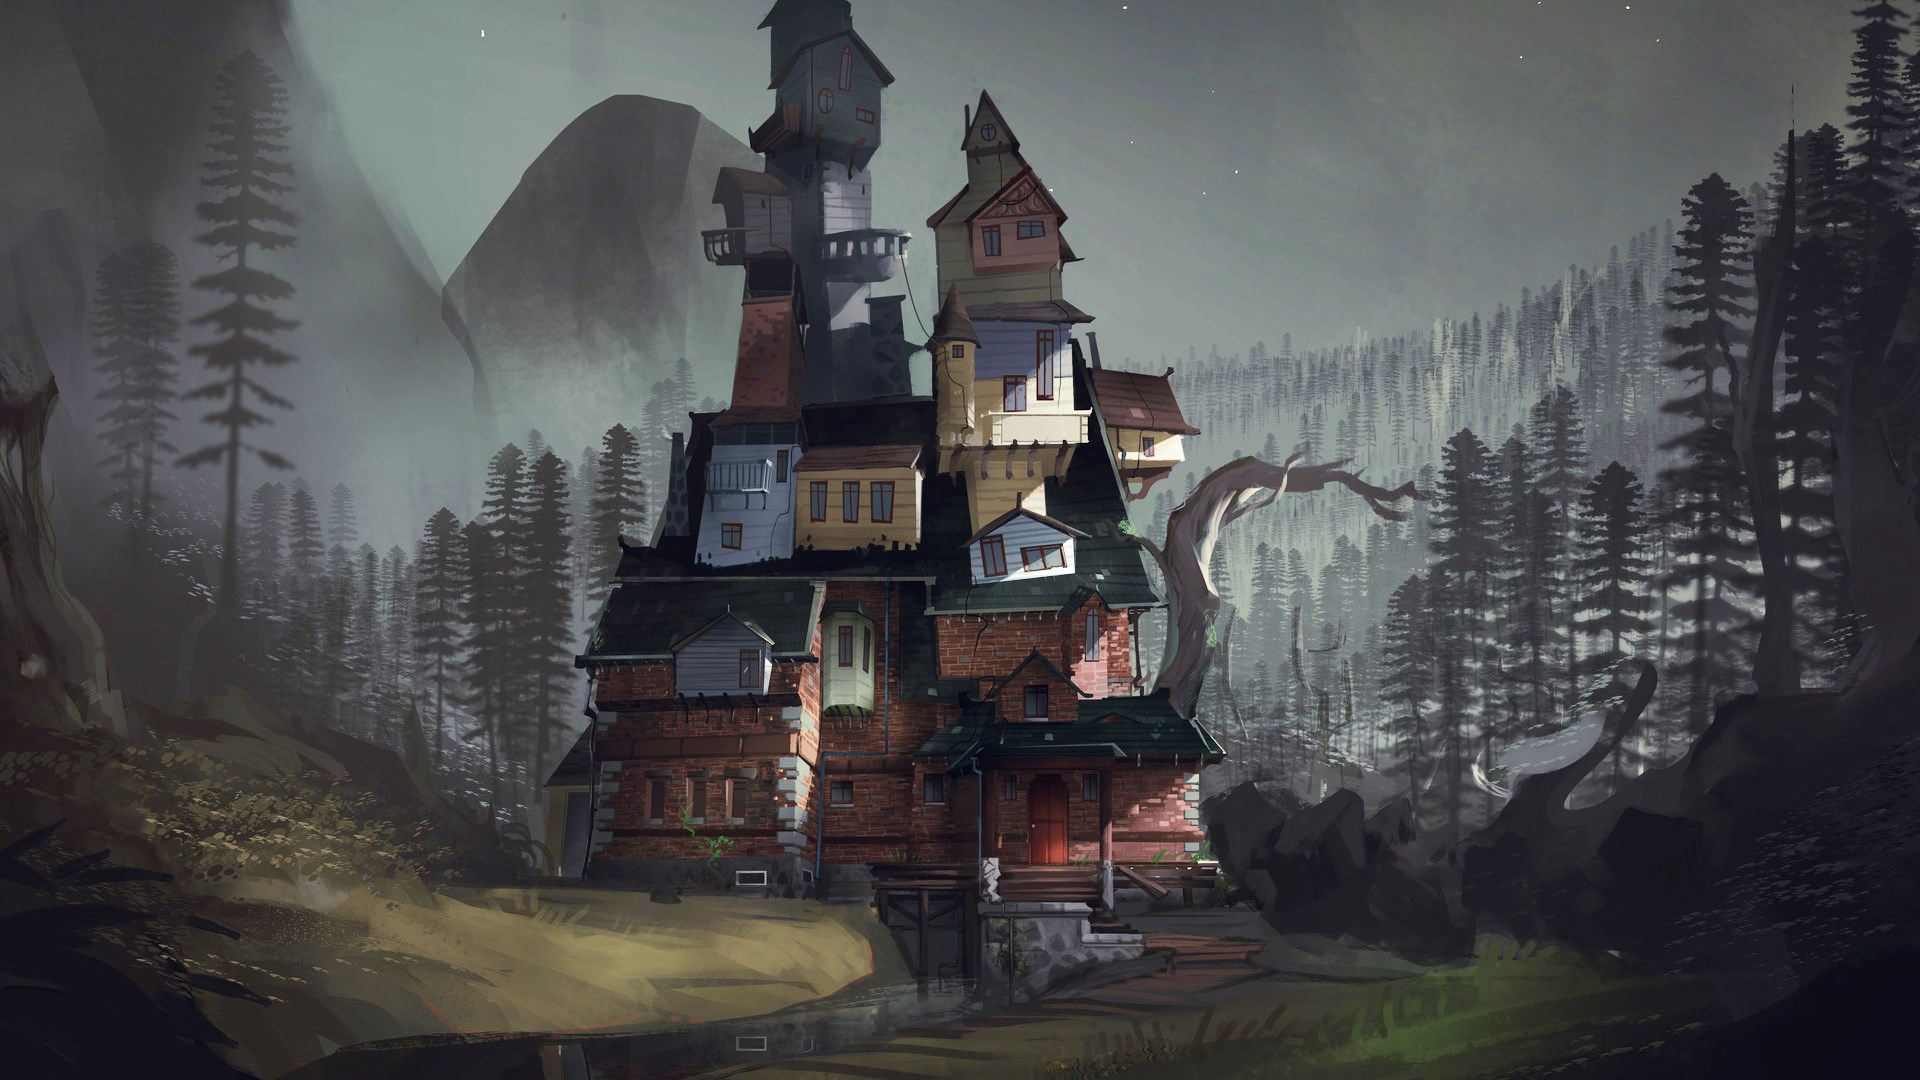
\includegraphics[width=\linewidth,height=.48\textheight,keepaspectratio]{assets/wroef.jpg}\end{center}\vfill
{\large Family, memories, possessions, and the stories we tell. Public and private identities through games, poetry, photography, podcasts, and television.\par}\clearpage

\clearpage\markboth{Who am I?}{}
\phantomsection\addcontentsline{toc}{section}{1. Who am I?}
{\color{blue}\small LESSON 01 \hfill 13 August 2026\par}
\vspace{4mm}
{\displayfont\color{navy}\fontsize{30}{34}\selectfont Who am I?\par}\vspace{4mm}

\section*{Program}

\begin{itemize}
\item \emph{08.35} Welcome
\item \emph{08.40} English C-level
\item \emph{08.45} Hangman of the day
\item \emph{08.50} Warm-up discussion
\item \emph{09.00} Who are you?
\item \emph{09.20} Break
\item \emph{09.30} Who are you? - continued
\item \emph{10.10} Break
\item \emph{10.25} Create meme
\item \emph{10.40} What Remains of Edith Finch? (trailer)
\item \emph{10.50} Exit-ticket
\item \emph{10.55} Identity in context
\end{itemize}

\section*{Hangman of the day}
\textbf{Hangman:} English term (7 characters).\par\medskip

\section*{Warm-up discussion}

\begin{itemize}
\item What is identity?
\item Why can it be a struggle during adolescence?
\item What are public and private parts of our identities?
\item How is identity formed?
Does it change over time?
\item What are the building blocks of identity?
\item Why do we have personal and public identities?
\item What parts of our identity can we change?
\item What aspects of our identity, if any, are fixed?
\item What choices do we make in regard to our personal identities?
\item Do we perform identity?
\end{itemize}

\section*{Personality}

\begin{itemize}
\item In his final act, the comedian takes on a child's personality
\item In this show, the competitor's \href{https://www.merriam-webster.com/dictionary/identity}{identity} will remain secret until after the vote.
\end{itemize}

\section*{Who are you?}

\begin{itemize}
\item Devide the sheet provided in half 4 times until you have 16 equal squares. Unfold the paper and cut each of these squares out.
\item Fill out the provided characteristic table
\end{itemize}

\section*{Who are you? - continued}

\begin{itemize}
\item Stack your pieces of paper so that the one that is least important is on top and the most important one is on the bottom. Complete the activity like this: 3-5 students share their least important piece of paper; everyone balls it up and they throw it into the trash can. Repeat that round until you get to the last 3. Sharing is optional. Throw away the 3rd most important. Students can keep the last 2 (most important pieces).
\item Reflect on the activity by answering the questions at the end of the provided hand-out.
\end{itemize}

\section*{Create a meme}

\noindent\begin{minipage}[c]{.51\linewidth}
Create a meme based on this template that represents how you see yourself, how your friends see you, how your family sees you, how your teacher sees you, how you “really are,” and one free choice.

\end{minipage}\hfill\begin{minipage}[c]{.44\linewidth}\centering

\includegraphics[width=\linewidth,height=.4\textheight,keepaspectratio]{assets/1782291276-meme.png}\end{minipage}\par\medskip

\section*{What Remains of Edith Finch? (trailer)}

\par\noindent\textbf{Video:} What Remains Of Edith Finch - Launch Trailer\par\medskip

\section*{Exit-ticket}

\begin{itemize}
\item Sum up today's lesson with one encompassing word. Try to come with a unique word that no one else in the class chooses.
\end{itemize}

\section*{Materials}

\begin{itemize}
\item \hyperref[worksheet-1]{Who are you? - handout (p.~\pageref*{worksheet-1})}
\item \hyperref[worksheet-2]{Identity in context (p.~\pageref*{worksheet-2})}
\end{itemize}

\clearpage\markboth{Masks}{}
\phantomsection\addcontentsline{toc}{section}{2. Masks}
{\color{blue}\small LESSON 02 \hfill 17 August 2026\par}
\vspace{4mm}
{\displayfont\color{navy}\fontsize{30}{34}\selectfont Masks\par}\vspace{4mm}

\section*{Program}

\begin{itemize}
\item \emph{12.05} Hangman of the day
\item \emph{12.15} Identity in context
\item \emph{12.25} Reading poems
\item \emph{12.30} We Wear the Mask
\item \emph{12.45} Break
\item \emph{12.55} Analysing poems

\begin{itemize}
\item Types of poems
\item FLIRT-model
\end{itemize}

\item \emph{13.25} Where Children Sleep

\begin{itemize}
\item Discuss
\item Write
\end{itemize}

\item \emph{13.55} Break
\item \emph{14.10} What Remains of Edith Finch?
\item \emph{14.30} Exit-ticket
\end{itemize}

\section*{Hangman of the day}
\textbf{Hangman:} Term from last lesson (11 characters).\par\medskip
\textbf{Hangman:} Term from last lesson (9 characters).\par\medskip
\textbf{Hangman:} Term from last lesson (14 characters).\par\medskip

\section*{Identity in context}

\begin{enumerate}
\item What are four words or phrases that describe you?
\item What are four hashtags you would use to describe yourself on a social media profile?
\item What are four words or phrases your friends or acquaintances would use to describe you?
\item What are four words or phrases your family would use to describe you?
\item What are your affiliations? These might include nationality, school, teams, clubs, etc.
\item List one or two strengths you would like to continue to develop.
\item What are some qualities you judge other people on?
\item “We contain multitudes," wrote Walt Whitman to describe that we express ourselves
differently in different contexts. What is an example of how your personality changes as you
associate with different groups of people? Why do you think it changes?
\end{enumerate}

\section*{Reading poems}

\begin{itemize}
\item Read the poem out loud!
\item Read it again.
\item Visit ambigous places, and look up difficult words.
\item Summarise the plot.
\end{itemize}

\section*{We Wear the Mask}

\begin{itemize}
\item Read the poem out loud!
\item Read it again.
\item Visit ambigous places, and look up difficult words.
\item Summarise the plot.
\end{itemize}

\section*{Analysing poems}

\begin{enumerate}
\item Determine the type of poem
\item Use the FLIRT-model to analyse the poem
\item Always remember to give examples from the poem to \textbf{substantiate} your analysis.
\end{enumerate}

\section*{Types of poems}

\begin{itemize}
\item \textbf{Didactic poems:} clear message or moral; meant to teach or explain something directly.\\\emph{Examples: "Do Not Stand at My Grave and Weep", "Eternity", "If—"}
\item \textbf{Dramatic monologue:} an imagined speaker addresses a silent listener; often a persona poem.\\\emph{Examples: "Maximus, to himself", "Lady Lazarus"}
\item \textbf{Elegy:} poem of mourning for someone who is dead; often moves from lament to praise to consolation.\\\emph{Examples: "O Captain! My Captain!", "The Haw Lantern"}
\item \textbf{Epic poems:} long narrative poems with a heroic protagonist, legendary adventures, and historical or mythical importance.\\\emph{Examples:}\emph{Beowulf, The Cantos, Paradise Lost}
\item \textbf{Epigrams:} very short poems, often witty or satirical, focused on a single thought or event.\\\emph{Example: "Candy is dandy, but liquor is quicker"}
\item \textbf{Prose poems:} written in prose form but read like poetry; often use repetition, symbols, and metaphors.\\\emph{Example: "Of Memory and Distance"}
\item \textbf{Limericks:} funny, light-hearted five-line poems with the rhyme scheme \textbf{aabba}.
\item \textbf{Slam poetry:} performance-based poetry with live audience participation; developed by Marc Kelly Smith in 1980s Chicago.
\end{itemize}

\section*{FLIRT-model}

\section*{F — Form}

\begin{itemize}
\item What structure does the poem have?
\item Does the structure have a certain effect on the reader?
\item Is there any correspondence between structure and content?
\end{itemize}

\section*{L — Language}

\begin{itemize}
\item What language is used?
\item Is the language emotive, persuasive, formal, informal etc.?
\item Which sentence structures, verbs, adjectives, and adverbs are used, and with what effect?
\end{itemize}

\section*{I — Imagery and rhetorical devices}

\begin{itemize}
\item Is there use of metaphors, similes, antithesis, onomatopoeia, allusion, repetition, or alliteration?
\item What is the effect?
\end{itemize}

\section*{R — Rhyme/rhythm}

\begin{itemize}
\item Does the poem rhyme?
\item Which rhyme scheme is used, and what is the effect?
\end{itemize}

\section*{T — Theme}

\begin{itemize}
\item Is there a message or theme in the poem?
\item Where is it visible?
\end{itemize}

\section*{Where Children Sleep}

\section*{Discuss}

\begin{itemize}
\item Look at and discuss Where Children Sleep
\begin{itemize}
\item What can we learn about the children based on their bedrooms?
\item How does this inform their identity?
\item Is this an expression of public or private identity?
\item Is it an invasion of their privacy?
\end{itemize}

\end{itemize}

\begin{center}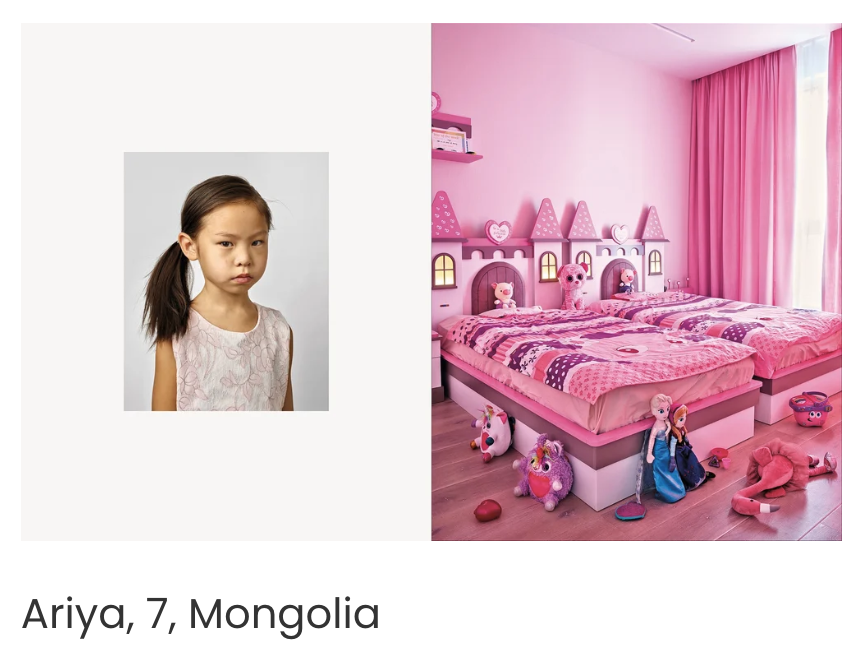
\includegraphics[width=\linewidth,height=.43\textheight,keepaspectratio]{assets/where_childre_sleep.png}\end{center}

\section*{Write}

\begin{enumerate}
\item Find a room that makes you appreciate your own room and explain why.
\item Find a room that reminds me of your room in some way.
\item Write about a room that interested you the most and why.
\end{enumerate}

\section*{What Remains of Edith Finch}

\par\noindent\textbf{Video:} What Remains of Edith Finch FULL GAME Walkthrough No Commentary (Longplay) (0:00–17:00)\par\medskip

\section*{Exit-ticket}

\begin{itemize}
\item Do the quick-write exercise on the handout.
\end{itemize}

\section*{Materials}

\begin{itemize}
\item \hyperref[worksheet-2]{Identity in context - handout (p.~\pageref*{worksheet-2})}
\item We Wear the Mask
\item Where Children Sleep
\end{itemize}

\clearpage\markboth{Identity of things}{}
\phantomsection\addcontentsline{toc}{section}{3. Identity of things}
{\color{blue}\small LESSON 03 \hfill 20 August 2026\par}
\vspace{4mm}
{\displayfont\color{navy}\fontsize{30}{34}\selectfont Identity of things\par}\vspace{4mm}

\section*{Program}

\begin{itemize}
\item \emph{08.35} Warm-up discussion
\item \emph{08.45} Molly's chapter

\begin{itemize}
\item Playthrough
\item Characterisation
\end{itemize}

\item \emph{09.20} Break
\item \emph{09.35} Reading fiction

\begin{itemize}
\item Analysing fiction
\item Exam

\begin{itemize}
\item Analysis
\end{itemize}

\end{itemize}

\item \emph{10.15} Break
\item \emph{10.25} Grammatik: Ordklasser
\item \emph{10.45} Reading
\end{itemize}

\section*{Warm-up discussion}

\begin{center}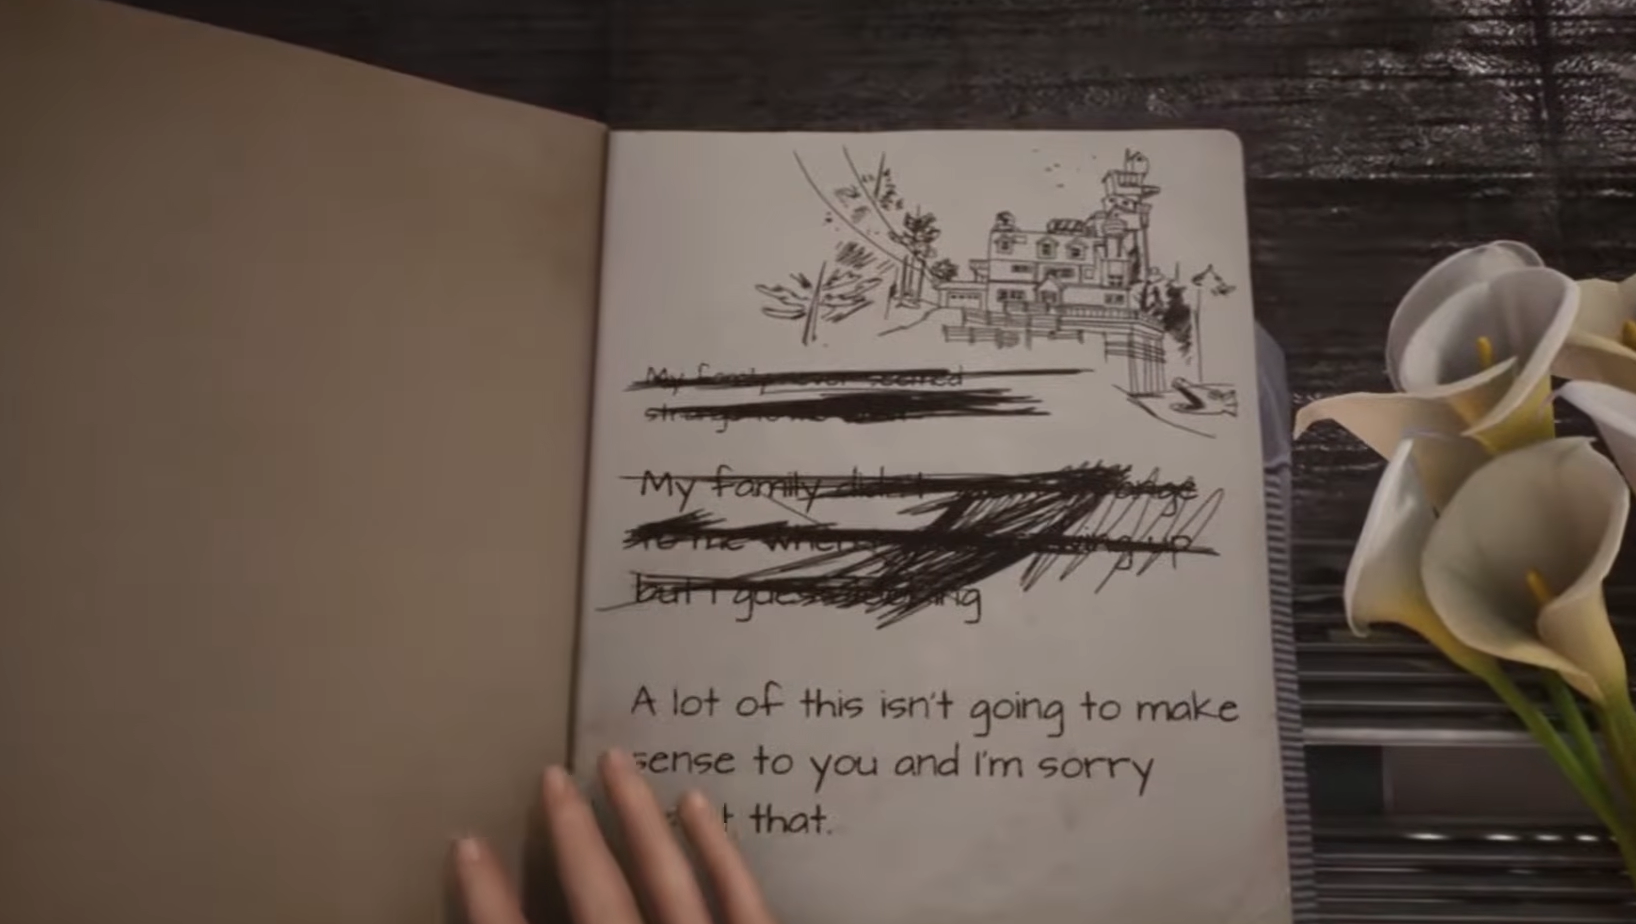
\includegraphics[width=\linewidth,height=.43\textheight,keepaspectratio]{assets/diary.png}\end{center}

\begin{itemize}
\item The entire story is told through Edith's journal. Can we trust what she tells us? Why or why not?
\item What is a flashback? Is the entire game a flashback?
\item Can we trust the narrator? Is she writing for a public or private audience? Is this more or less likely to make her presentation truthful?
\end{itemize}

\section*{Playthrough}

\par\noindent\textbf{Video:} What Remains of Edith Finch FULL GAME Walkthrough No Commentary (Longplay) (17:00–30:45)\par\medskip

\section*{Characterisation}

\begin{itemize}
\item How can personal items and possessions project identity?
\item How and why do we project status through our possessions?
\item Judging by the items in her room, how is Molly's experience an expression of her identity?
\item If Molly identifies with nature and animals, how does that affect the choices she makes?
\end{itemize}

\section*{Analysing fiction}

\section*{Plot/structure}

\begin{itemize}
\item How is the story built up?
\item Is it chronological, with flashbacks, open ending, climax, turning point?
\end{itemize}

\section*{Characterisation}

\begin{itemize}
\item How are characters presented?
\item Directly or indirectly?
\item How do they develop?
\end{itemize}

\section*{Setting}

\begin{itemize}
\item Where and when does the story take place?
\item What is the social/cultural environment?
\item How does the setting affect characters and theme?
\end{itemize}

\section*{Narrator / point of view}

\begin{itemize}
\item Who tells the story?
\item What is the effect of this perspective?
\item Is the narrator reliable?
\end{itemize}

\section*{Language}

\begin{itemize}
\item What kind of language is used?
\item Formal/informal, descriptive, symbolic, emotional?
\item Are there rhetorical devices or imagery?
\end{itemize}

\section*{Theme/message}

\begin{itemize}
\item What central themes are explored?
\item What message or comment does the text seem to make?
\end{itemize}

\section*{Exam}

\begin{itemize}
\item 6-8 minute presentation

\begin{enumerate}
\item Summary
\item Analysis
\item Relate to theme
\end{enumerate}

\item Dialogue
\end{itemize}

\section*{Analysis}

\begin{itemize}
\item ACE

\begin{itemize}
\item \emph{A}nswer
\item \emph{C}ite
\item \emph{E}xplain
\end{itemize}

\item PEE

\begin{itemize}
\item \emph{P}oint
\item \emph{E}vidence
\item \emph{E}xplanation
\end{itemize}

\end{itemize}

\section*{Grammatik: Ordklasser}
Verbum, substantiv, artikel, pronomen, adjektiv, adverbium, præposition, konjunktion, numerale, interjektion


\section*{Reading}

\par\noindent\textbf{Video:} "The Veldt" by Ray Bradbury (Read Aloud w/ text)\par\medskip

\section*{Ordklasser}

{\small\setlength{\tabcolsep}{4pt}\renewcommand{\arraystretch}{1.3}\begin{tabularx}{\linewidth}{@{}>{\raggedright\arraybackslash}X>{\raggedright\arraybackslash}X>{\raggedright\arraybackslash}X>{\raggedright\arraybackslash}X@{}}\toprule
Latin & Dansk & Forklaring & Eksempler\\
Verbum & Udsagnsord & Ord, der kan bøjes i tid & \emph{say, go, get, take}\\
Substantiv & Navneord & Ord, der kan sættes \emph{the} foran & \emph{year, day, thing}\\
Artikel & Kendeord & Bestemmelsesord til substantiver & \emph{a, an, the}\\
Pronomen & Stedord & Ord, der kan stå i stedet for et substantiv & \emph{it, you, their, who}\\
Adjektiv & Tillægsord & Ord, der beskriver substantiver og pronomener & \emph{new, good, different}\\
Adverbium & Biord & Ord, der beskriver verbal-led, adjektiver, adverbier eller sætninger & \emph{very, really, simply, here}\\
Præposition & Forholdsord & Ord, der viser en position i forhold til et substantiv & \emph{in, on, from, before, during}\\
Konjunktion & Bindeord & Ord, der binder sætninger og ord sammen & \emph{and, or, but, because, when}\\
Numerale & Talord & Ord, der kan skrives som tal & \emph{two, four, third, tenth, a thousand}\\
Interjektion & Udråbsord & Ord, der udtrykker udråb & \emph{ah, oh, gosh}\\
\bottomrule\end{tabularx}}\par\medskip

\section*{Materials}

\begin{itemize}
\item \hyperref[worksheet-3]{Molly's chapter - pacing questions (p.~\pageref*{worksheet-3})}
\item \hyperref[worksheet-4]{Molly's Room (p.~\pageref*{worksheet-4})}
\item \hyperref[worksheet-5]{Grammatik: Ordklasser (p.~\pageref*{worksheet-5})}
\item The Veldt
\end{itemize}

\clearpage\markboth{The stories that shape us}{}
\phantomsection\addcontentsline{toc}{section}{4. The stories that shape us}
{\color{blue}\small LESSON 04 \hfill 24 August 2026\par}
\vspace{4mm}
{\displayfont\color{navy}\fontsize{30}{34}\selectfont The stories that shape us\par}\vspace{4mm}

\section*{Program}

\begin{itemize}
\item \emph{12.05} Warm-up read and discussion
\item \emph{12.25} Calvin

\begin{itemize}
\item Playthrough
\end{itemize}

\item \emph{12.45} Characterisation
\item \emph{13.00} Break
\item \emph{13.10} Twine-creations
\item \emph{14.10} Break
\item \emph{14.25} Twine playing asdklfja
\end{itemize}

\section*{Warm-up read and discussion}

\begin{enumerate}
\item How do people usually describe themselves when they tell their life story?
\item Do you think people focus more on positive or negative experiences when talking about their past? Why?
\item Can a bad experience help a person grow? In what ways?
\item Why do some people see challenges as important turning points in life?
\item Do you think the way we talk about our past can change how we feel about ourselves? Why or why not?
\item Is it possible to “rewrite” your personal story without changing the facts? How?
\end{enumerate}

\section*{Playthrough}

\par\noindent\textbf{Video:} What Remains of Edith Finch FULL GAME Walkthrough No Commentary (Longplay) (30:45–44:00)\par\medskip

\section*{Characterisation}

\begin{itemize}
\item Comment on this quote: "This will be obvious later, but my mom never told me any of these stories. Edie would have, but Mom didn't like bringing up the past. Though when we adopted a stray kitten she was the one who named it "Molly"". What do the stories mean to Dawn? What do they mean to Edie?
\item Look at Sam and Calvin’s room. How do you know they are twins?
\item How is it visually inferred? And how is it plainly stated?
\item What is odd about the room?
\item How did Calvin deal with the trauma of Barbara’s death?
\item Did his disobedience lead to death? What evidence is there that Calvin is defiant? Did he die happy?
\item Why is his leg in a cast? What does it say about Calvin?
\item What does the letter in the astronaut helmet symbolize?
\end{itemize}

\section*{Twine-creations}

\begin{itemize}
\item Create a 3-passage \href{https://twinery.org}{Twine}. The first should be a neutral description of Calvin’s demise. Then create a link to a passage that describes his death as a redemptive narrative and a second link to a passage that describes Calvin’s demise as contamination narrative.
\item Create another minimum 3-passage Twine. It can be one that describes an incident in your life that was life-changing or contributed to the development of your identity with a redemptive arc and contamination arc. If you feel inspired you can also choose your own topic and structure.
\end{itemize}

\section*{Twine playing}

\begin{itemize}
\item Play/read at least three of your classmate's Twines.
\end{itemize}

\section*{Materials}

\begin{itemize}
\item \hyperref[worksheet-6]{Calvin and Odin - pacing questions (p.~\pageref*{worksheet-6})}
\item Two kinds of stories - article
\end{itemize}

\clearpage\markboth{Influencers}{}
\phantomsection\addcontentsline{toc}{section}{5. Influencers}
{\color{blue}\small LESSON 05 \hfill 27 August 2026\par}
\vspace{4mm}
{\displayfont\color{navy}\fontsize{30}{34}\selectfont Influencers\par}\vspace{4mm}

\section*{Program}

\begin{itemize}
\item \emph{08.35} Warm-up discussion
\item \emph{08.40} Barbara

\begin{itemize}
\item Playthrough
\item Language
\end{itemize}

\item \emph{09.15} Break
\item \emph{09.30} Grammatik: Sætningsanalyse

\begin{itemize}
\item Subjekt og verballed
\end{itemize}

\item \emph{10.30} Break
\item \emph{10.45} Walk'n'listen
\end{itemize}

\section*{Warm-up discussion}

\begin{itemize}
\item Identify a role model from your childhood that had an afect on your identity formation.
\item Identify a role model that you currently admire.
\item What are the qualities or traits you admire in this person? Are they qualities that you are trying to develop in yourself? Has this person had any efect on the formation of your identity?
\end{itemize}

\section*{Playthrough}

\begin{center}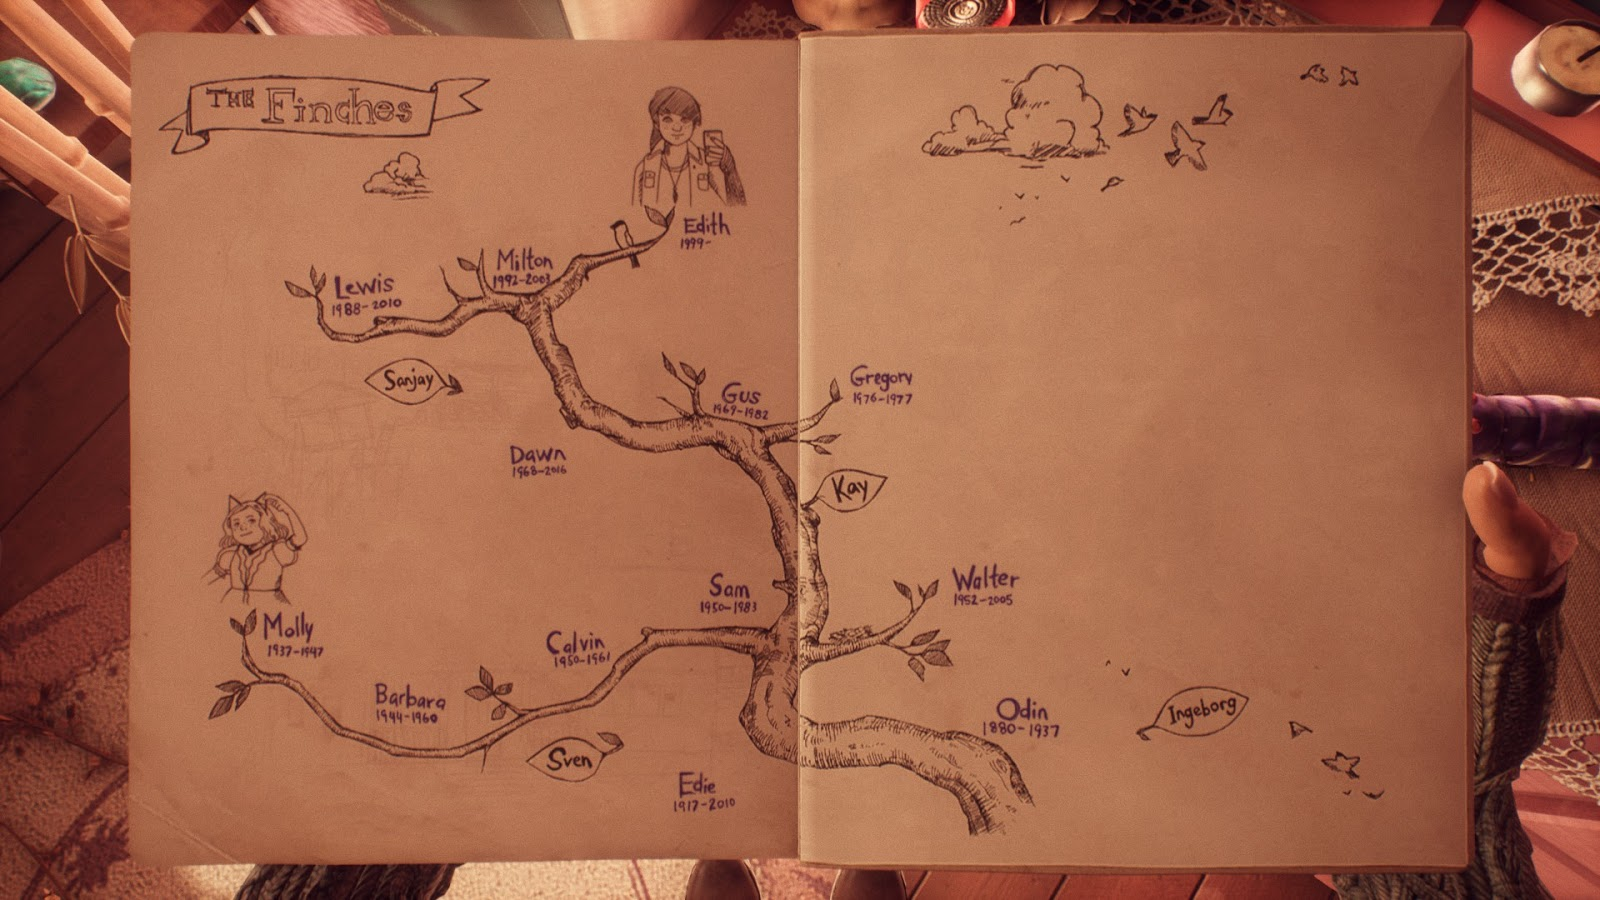
\includegraphics[width=\linewidth,height=.43\textheight,keepaspectratio]{assets/finch-family-tree.png}\end{center}

\par\noindent\textbf{Video:} What Remains of Edith Finch FULL GAME Walkthrough No Commentary (Longplay) (44:00–57:00)\par\medskip

\section*{Language}

\begin{itemize}
\item Fill out the table on the handout
\item Write an ACE / PEE paragraph, explaining how Barbara died. You must cite direct evidence from the chapter.

\begin{itemize}
\item ACE

\begin{itemize}
\item \emph{A}nswer
\item \emph{C}ite
\item \emph{E}xplain
\end{itemize}

\item PEE

\begin{itemize}
\item \emph{P}oint
\item \emph{E}vidence
\item \emph{E}xplanation
\end{itemize}

\end{itemize}

\end{itemize}

\section*{Grammatik: Sætningsanalyse}

\begin{itemize}
\item Lav opgaver om sætningsanalyse på \href{https://app.minlaering.dk/lektier?vis=411995}{minlæring.dk}
\end{itemize}

\section*{Walk'n'listen}

\begin{itemize}
\item Look up Willie Nelson on the internet
\item Listen to the first act of the below episode
\end{itemize}
\textbf{This American Life — "Golden Calf", Act One: "Bowing Before The Famous"}


\begin{itemize}
\item Transcript
\item \href{https://www.thisamericanlife.org/185/golden-calf/act-one-0}{Open episode page}
\end{itemize}

\section*{Reflect}

\begin{itemize}
\item What are some characteristics of Willie Nelsons's public identity? Do you think they also describe his private identity? Why?
\item What is the role of Willie Nelson in the lives of his fans?
\item What do people we don't know personally mean to our identity?
\end{itemize}
Submit an audioanswer to these questions \href{https://app.edaptio.com/groups/857421/courses/61482/lesson/278058}{here}.


\section*{Materials}

\begin{itemize}
\item \hyperref[worksheet-7]{Barbara's chapter (p.~\pageref*{worksheet-7})}
\item Sætningsanalyse på minlæring.dk
\end{itemize}

\clearpage\markboth{Secrets}{}
\phantomsection\addcontentsline{toc}{section}{6. Secrets}
{\color{blue}\small LESSON 06 \hfill 31 August 2026\par}
\vspace{4mm}
{\displayfont\color{navy}\fontsize{30}{34}\selectfont Secrets\par}\vspace{4mm}

\section*{Program}

\begin{itemize}
\item \emph{12.05} PostSecret
\item \emph{12.20} Walter

\begin{itemize}
\item Playthrough
\end{itemize}

\item \emph{12.50} Break
\item \emph{13.05} Discussion
\item \emph{13.15} Writing
\item \emph{13.50} Break
\item \emph{14.00} Grammar: Verballed
\end{itemize}

\section*{PostSecret}

\begin{itemize}
\item Look at the \href{https://postsecret.com}{PostSecret} website. Discuss why this site exists and why people would send their secrets.
\item What does this reveal about our private identities?
\item What's the difference between this and social media?
\end{itemize}

\section*{Playthrough}

\par\noindent\textbf{Video:} What Remains of Edith Finch FULL GAME Walkthrough No Commentary (Longplay) (56:45–76:00)\par\medskip

\section*{Discussion}

\begin{itemize}
\item Why has Walter isolated himself? How has this afected his relationship with the world?
\item What is Walter afraid of? How has fear shaped his life?
\item Looking at his postcards, is he the person he wants to be? What’s holding him back?
\item What feelings do you think Walter was having just before he died? What is ironic about his death?
\end{itemize}

\section*{Writing}

\begin{itemize}
\item Write a PostSecret for any two of the following: Molly, Barbara, Calvin, or Walter. Then, find an image that would be on the postcard and explain how it relates to the character/secret.
\item Design a support system for this character. Would they call a hotline? Imagine a better route, the safety net and skill this character could have had.
\item Why does PostSecret exist? Why do we need it at all? Would sending this postcard have helped? Can it backfire? Write a response.
\end{itemize}

\section*{Grammar: Sætningsanalyse}

\section*{Materials}

\begin{itemize}
\item \hyperref[worksheet-8]{Walter's chapter (p.~\pageref*{worksheet-8})}
\item \hyperref[worksheet-9]{Sætningsanalyse - arbejdsark (p.~\pageref*{worksheet-9})}
\end{itemize}

\clearpage\markboth{Split in two}{}
\phantomsection\addcontentsline{toc}{section}{7. Split in two}
{\color{blue}\small LESSON 07 \hfill 3 September 2026\par}
\vspace{4mm}
{\displayfont\color{navy}\fontsize{30}{34}\selectfont Split in two\par}\vspace{4mm}

\section*{Program}

\begin{itemize}
\item \emph{08.35} Warm up
\item \emph{08.55} Analysing fiction (continued)

\begin{itemize}
\item Overview of cinematic techniques
\end{itemize}

\item \emph{09.05} Severance
\item \emph{09.40} Break
\item \emph{09.55} Discuss plot
\item \emph{10.05} Analyse cinematic technique
\item \emph{10.35} Break
\item \emph{10.45} Grammatik: Verber
\end{itemize}

\section*{Warm up}

\begin{enumerate}
\item Read the article The Fly Nobody Programmed
\item Discuss

\begin{itemize}
\item How does the fly "choose" to do what it does?
\item What's the difference between this and LLM's?
\item Does the fly have an identity? On what is it based?
\item Would a human digitised brain be conscious? Would it have an identity? Would it be the same as the original organic brain?
\end{itemize}

\end{enumerate}

\section*{Analysing fiction (continued)}

\begin{itemize}
\item Plot/structure


\item Characterisation


\item Setting


\item Narrator / point of view


\item Language


\item Theme/message


\begin{itemize}
\item How does \emph{language} support the story?
\item How does \emph{game mechanics} support the story?
\item How does \emph{cinematic technique} support the story?
\item How do \emph{graphics} support the story?
\end{itemize}

\end{itemize}

\section*{Overview of cinematic techniques}

{\small\setlength{\tabcolsep}{4pt}\renewcommand{\arraystretch}{1.3}\begin{tabularx}{\linewidth}{@{}>{\raggedright\arraybackslash}X>{\raggedright\arraybackslash}X@{}}\toprule
Cinematic technique & Characteristics\\
\textbf{Framing} & \textbf{Close-up:} The character(s) are framed very closely.\newline{}\newline{}\textbf{Long shot:} Focus is on setting.\newline{}\newline{}\textbf{Medium shot:} Focus is on more than one character.\\
\textbf{Angles} & \textbf{Low angle:} The character in question seems powerful and big.\newline{}\newline{}\textbf{High angle:} The character in question seems small and maybe weak.\newline{}\newline{}\textbf{Eye level:} Audience at the same level as characters.\\
\textbf{Composition} & Foreground.\newline{}\newline{}Middle ground.\newline{}\newline{}Background.\\
\textbf{Sound} & \textbf{Diegetic sound:} Sound which is part of the film.\newline{}\newline{}\textbf{Non-diegetic sound:} Sound which is not part of the film.\newline{}\newline{}\textbf{Contrapuntal sound:} Sound in direct contrast to the images of the film.\\
\textbf{Lighting} & \textbf{Low key:} Difficult to see everything in the image.\newline{}\newline{}\textbf{High key:} Able to see everything in the image.\\
\textbf{Colour} & Each colour has both a positive and negative symbolism.\\
\bottomrule\end{tabularx}}\par\medskip

\section*{Discuss plot}

\begin{itemize}
\item In your own words, explain the severance procedure.
\item Who is Helly? Is there a difference between her work self and her private self?
\item Is it fair to say that Helly chooses to come back to work?
\item Do we sometimes subject ourselves to similar things? Do you?
\end{itemize}

\section*{Analyse cinematic technique}

\begin{itemize}
\item Describe - in bullets - three examples of cinematic techniques in the excerpt and explain for each why you think they are used.
\end{itemize}

\section*{Grammatik: Verber}

\section*{Forskellen på verber og verballed}
\begin{taskbox}
I have a wallet

I lost my wallet

I have lost my wallet

We enjoy working with short stories

\end{taskbox}

\section*{Verbalformer}

{\small\setlength{\tabcolsep}{4pt}\renewcommand{\arraystretch}{1.3}\begin{tabularx}{\linewidth}{@{}>{\raggedright\arraybackslash}X>{\raggedright\arraybackslash}X>{\raggedright\arraybackslash}X@{}}\toprule
Latin & Dansk & Eksempler\\
INFINITIV & Navneform & \emph{to ask}\\
PERFEKTUM PARTICIPIUM & Kort tillægsform & \emph{asked}\\
PRÆSENS PARTICIPIUM & Lang tillægsform, \emph{ing}-form & \emph{asking}\\
IMPERATIV & Bydeform & \emph{ask!}\\
\bottomrule\end{tabularx}}\par\medskip

\section*{Verbets tider}

{\small\setlength{\tabcolsep}{4pt}\renewcommand{\arraystretch}{1.3}\begin{tabularx}{\linewidth}{@{}>{\raggedright\arraybackslash}X>{\raggedright\arraybackslash}X>{\raggedright\arraybackslash}X>{\raggedright\arraybackslash}X>{\raggedright\arraybackslash}X@{}}\toprule
Præsens & Præteritum & Perfektum & Pluskvamperfektum & Futurum\\
\emph{I talk} & \emph{talked} & \emph{have talked} & \emph{had talked} & \emph{will talk}\\
\emph{you talk} & \emph{talked} & \emph{have talked} & \emph{had talked} & \emph{will talk}\\
\emph{he/she/it talks} & \emph{talked} & \emph{has talked} & \emph{had talked} & \emph{will talk}\\
\emph{we talk} & \emph{talked} & \emph{have talked} & \emph{had talked} & \emph{will talk}\\
\emph{you talk} & \emph{talked} & \emph{have talked} & \emph{had talked} & \emph{will talk}\\
\emph{they talk} & \emph{talked} & \emph{have talked} & \emph{had talked} & \emph{will talk}\\
\bottomrule\end{tabularx}}\par\medskip

\section*{Materials}

\begin{itemize}
\item The Fly Nobody Programmed
\end{itemize}

\clearpage\markboth{The curse of stories}{}
\phantomsection\addcontentsline{toc}{section}{8. The curse of stories}
{\color{blue}\small LESSON 08 \hfill 10 September 2026\par}
\vspace{4mm}
{\displayfont\color{navy}\fontsize{30}{34}\selectfont The curse of stories\par}\vspace{4mm}

\section*{Program}

\begin{itemize}
\item \emph{08.35} Warm up
\item \emph{08.50} Edith
\item \emph{09.05} Discussion
\item \emph{09.25} Break
\item \emph{09.40} Questions for \emph{What Remains of Edith Finch}?

\begin{itemize}
\item Bloom's taxonomy

\begin{itemize}
\item Examples
\end{itemize}

\item Writing questions
\end{itemize}

\item \emph{10.30} Break
\item \emph{10.40} Answering questions
\item \emph{11.05} Summary
\end{itemize}

\section*{Warm up}

\begin{itemize}
\item Draw a timeline of events (deaths) so far in What Remains of Edith Finch? Next to names draw one object to symbolise how that character died.
\end{itemize}

\begin{center}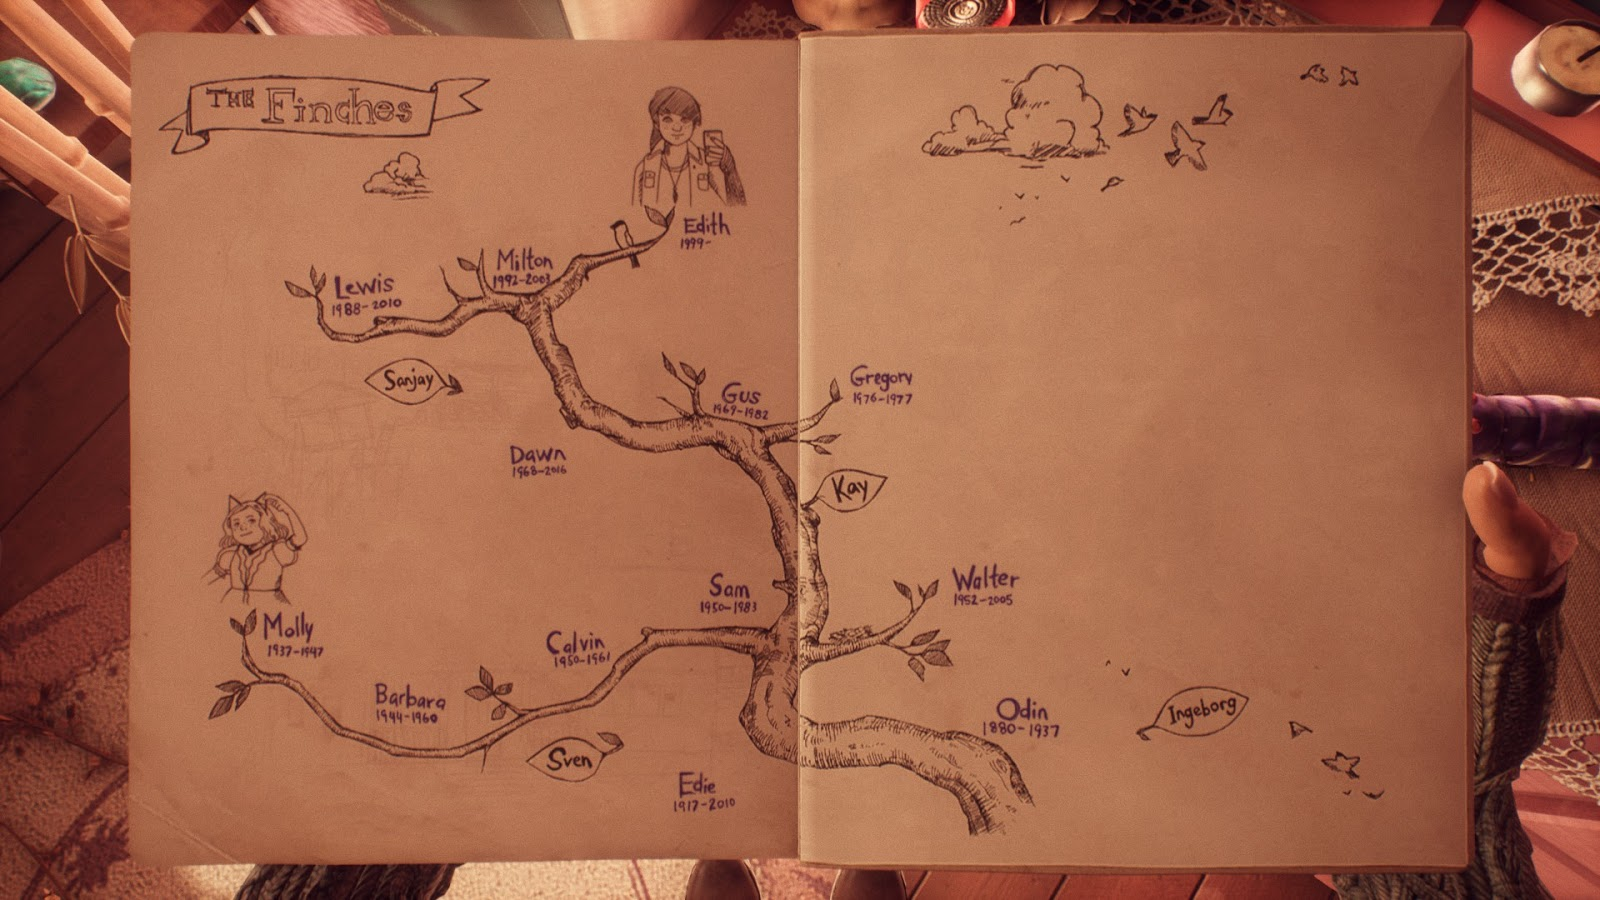
\includegraphics[width=\linewidth,height=.43\textheight,keepaspectratio]{assets/finch-family-tree.png}\end{center}

\section*{Edith}

\par\noindent\textbf{Video:} What Remains of Edith Finch FULL GAME Walkthrough No Commentary (Longplay) (121:00 onwards)\par\medskip

\section*{Discussion}

\begin{enumerate}
\item What do we learn about Edith’s reason for returning to the Finch house, and how does this change our understanding of the game’s story?


\item How does the final vignette connect Edith’s pregnancy to the themes of family, memory, and inheritance?


\item What does Edith seem to believe about the “Finch curse” by the end of the game? Does she accept it, reject it, or something in between?


\item How does the ending change the role of the player? What does it mean that the story is ultimately being read by Edith’s child?


\item After finishing the game, what do you think the title What Remains of Edith Finch means? What “remains” of Edith, her family, and their stories?


\end{enumerate}

\section*{Bloom's taxonomy}

\begin{center}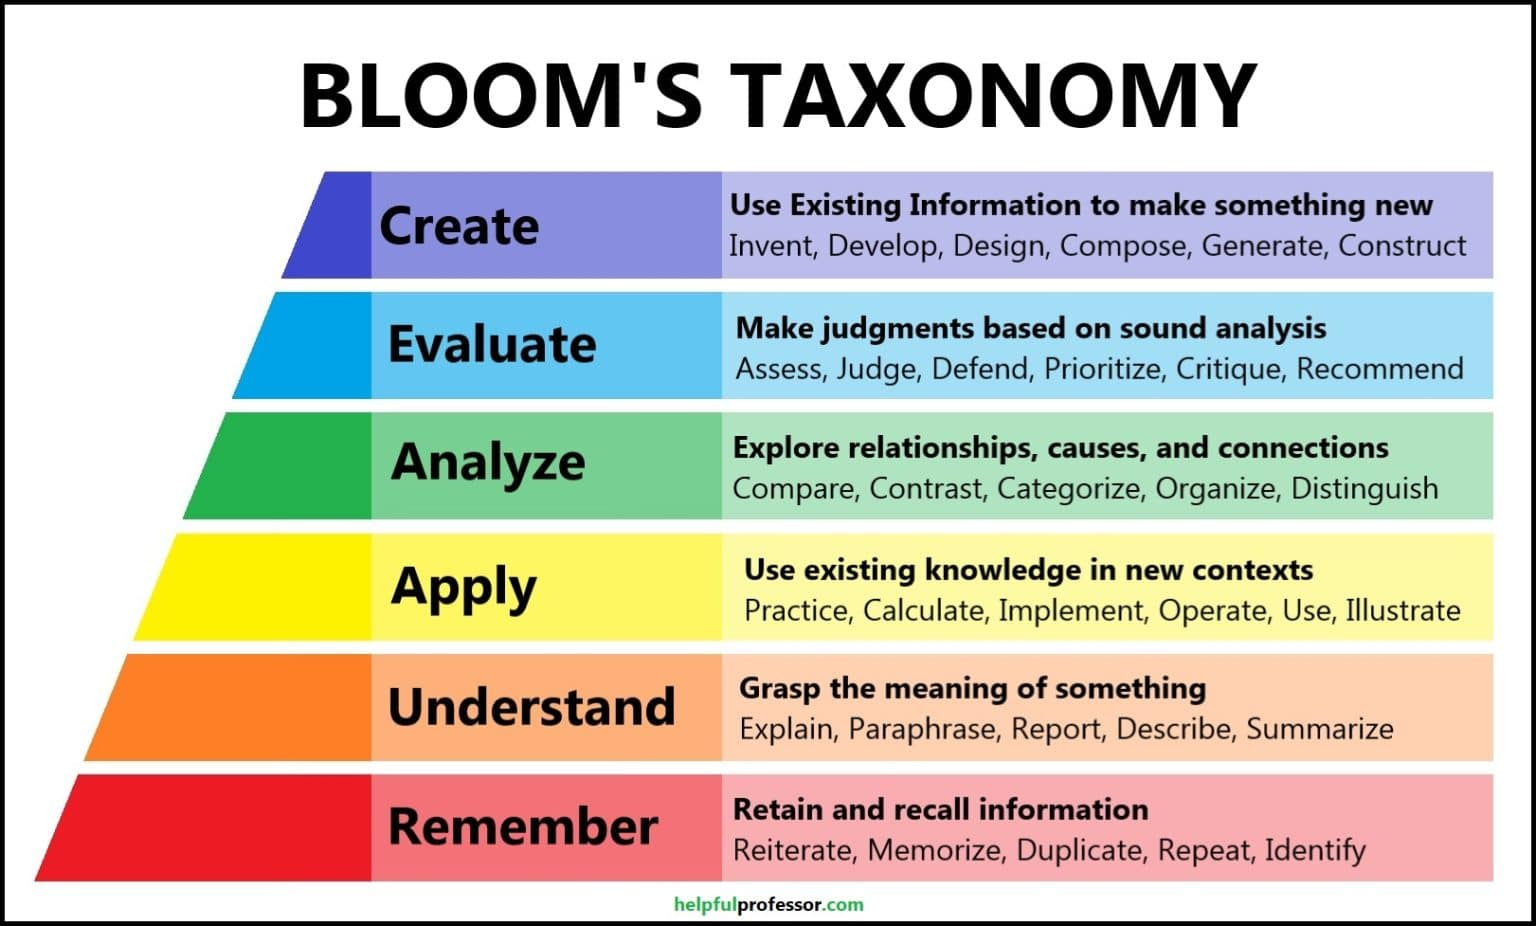
\includegraphics[width=\linewidth,height=.43\textheight,keepaspectratio]{assets/1788265373-bloom.png}\end{center}

\section*{Examples}

\begin{enumerate}
\item \textbf{Remember}\\
What are the five questions in the questionnaire given to Helly when she wakes up at the table?


\item \textbf{Understand}\\
Explain what the severance procedure does to a person’s memory and identity.


\item \textbf{Apply}\\
If you were explaining Lumon’s severance system to someone who had never seen the show, what real-life workplace situation could you compare it to?


\item \textbf{Analyze}\\
How does the episode create a contrast between Mark’s “innie” life at work and his “outie” life outside Lumon?


\item \textbf{Evaluate}\\
Do you think Helly’s choice to undergo severance is understandable?


\item \textbf{Create}\\
If you were a journalist tasked with writing an article about the procedure, and you had an interview with Helly, what would you ask her?


\end{enumerate}

\section*{Writing questions}

\begin{enumerate}
\item Create 6 questions freely
\item Create 6 questions following Bloom's taxonomy
\end{enumerate}

\begin{center}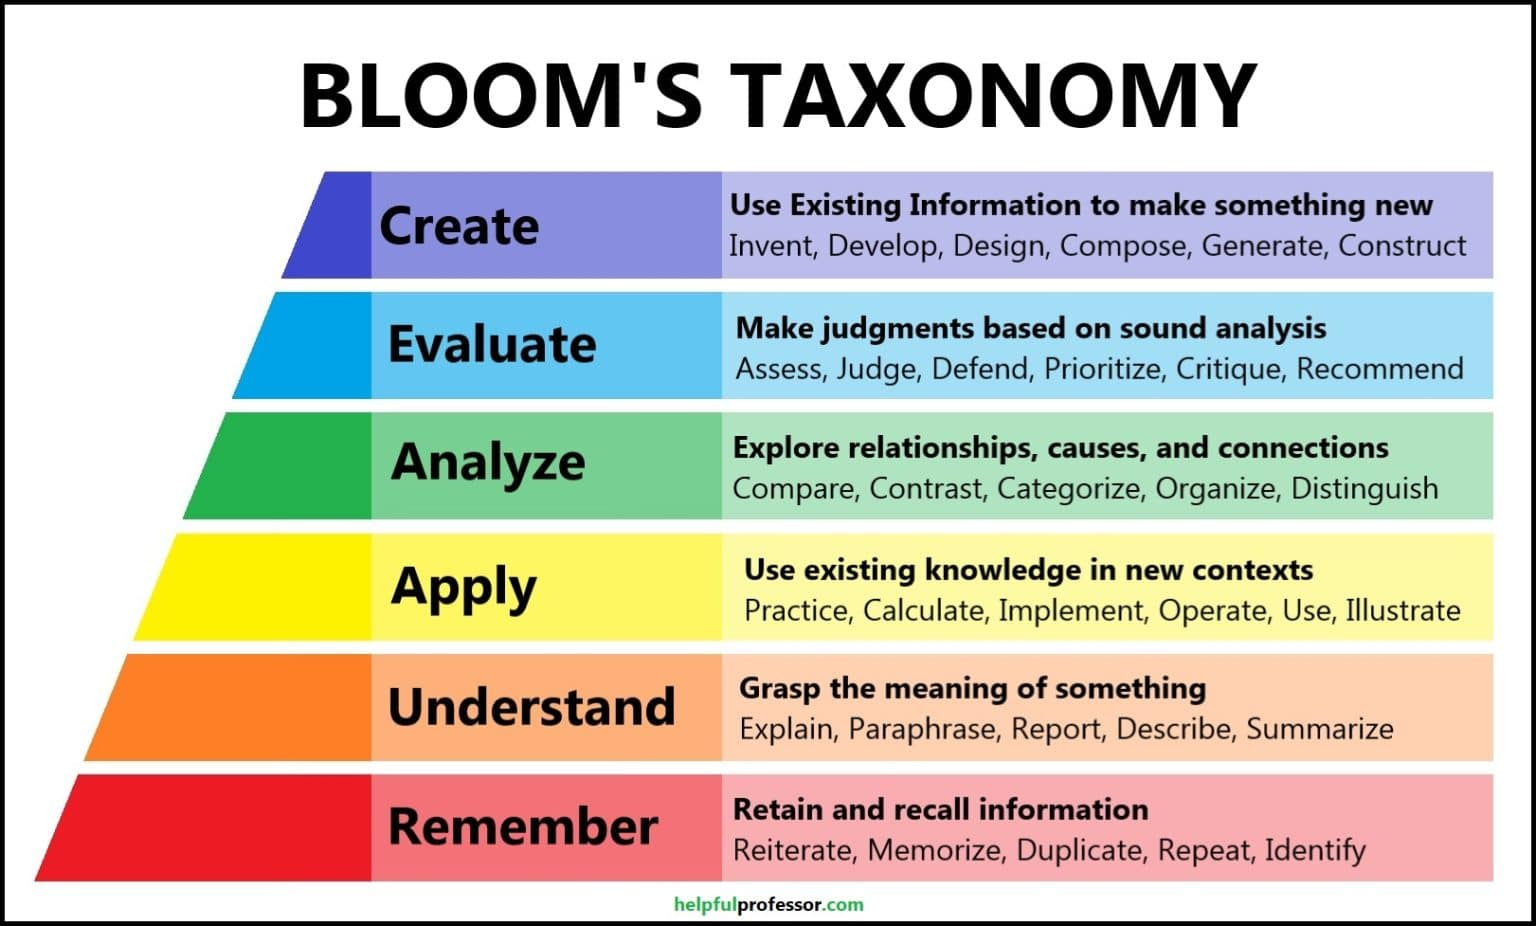
\includegraphics[width=\linewidth,height=.43\textheight,keepaspectratio]{assets/1788265373-bloom.png}\end{center}

\section*{Answering questions}

\begin{itemize}
\item Answer questions in writing

\begin{itemize}
\item Use as many examples and explanations as you can
\item Optionally add association comments connected to the questions
\end{itemize}

\end{itemize}

\section*{Summary}

\begin{itemize}
\item Look at the answers: Do you agree with them? Can you add something?
\end{itemize}

\section*{Materials}

\begin{itemize}
\item \hyperref[worksheet-10]{Edith - pacing questions (p.~\pageref*{worksheet-10})}
\end{itemize}

\clearpage\phantomsection\addcontentsline{toc}{chapter}{2. Voice}\markboth{Voice}{}\thispagestyle{empty}
\fancyhead[L]{\small\color{blue}Voice}
\vspace*{12mm}
{\color{blue}\large CHAPTER 2\par}\vspace{8mm}
{\displayfont\color{navy}\fontsize{43}{47}\selectfont Voice\par}\vspace{12mm}
\begin{center}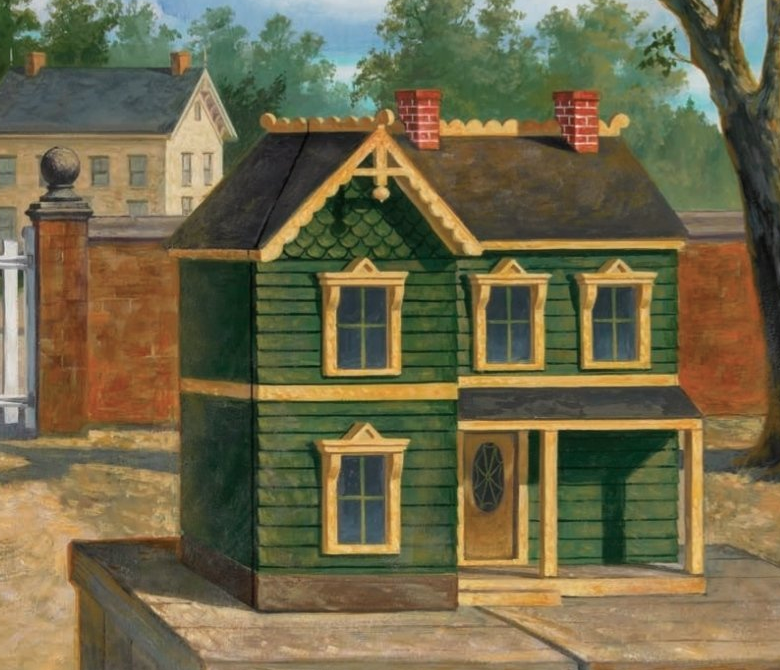
\includegraphics[width=\linewidth,height=.48\textheight,keepaspectratio]{assets/dolls-house-button.png}\end{center}\vfill
{\large Finding your voice and hearing someone else’s. Narrative voices, self-expression, speeches, and the relationship between personal confidence and public responsibility.\par}\clearpage

\clearpage\markboth{Voice}{}
\phantomsection\addcontentsline{toc}{section}{1. Voice}
{\color{blue}\small LESSON 01 \hfill 14 September 2026\par}
\vspace{4mm}
{\displayfont\color{navy}\fontsize{30}{34}\selectfont Voice\par}\vspace{4mm}

\section*{Program}

\begin{itemize}
\item \emph{12.05} Rights of the reader
\item \emph{12.20} Vocabulary
\item \emph{12.35} Reading
\item \emph{12.45} Break
\item \emph{13.00} First impression
\item \emph{13.10} Reading continued
\item \emph{13.50} Break
\item \emph{14.00} Writing

\begin{itemize}
\item Explanation
\item Free genre
\end{itemize}

\end{itemize}

\section*{Rights of the reader}

\begin{itemize}
\item Look up Daniel Pennac's Rights of the reader
\item Which of the rights of the reader do you consider most important? Why?
\item Are any of the rights unnecessary? Which and why?
\item Farrah Serroukh from the Centre for Literacy in Primary Education proposes the 11th Right of the Reader: the right of every reader to be visible. How do you interpret this right, and how important do you think it is?
\item If you were to add the 12th Right of the Reader, what would you suggest and why?
\item Discuss these questions:

\begin{itemize}
\item What do you read for pleasure? – and for information?
\item When do you read for pleasure? – and for information?
\item Where do you read for pleasure? – and for information?
\item Do you read for pleasure in school? – and for information?
\item What was the last text you read for pleasure?
\item Why do you (not) read for pleasure? – and for information?
\end{itemize}

\end{itemize}

\section*{Vocabulary}

\begin{itemize}
\item For each of the following adjectives find a synonym and an antonym: \emph{shattering} · \emph{terrible} · \emph{liberating} · \emph{stimulating} · \emph{appalling} · \emph{wonderful} · \emph{incredible}
\item With what would you connect the following nouns? Suggest a superordinate term (overordnet begreb) for: \emph{titillation} · \emph{possibility} · \emph{chance of encounter} · \emph{vindication}
\item Suggest a superordinate term for these verbs: \emph{bowed down before} · \emph{worshipped} · \emph{embraced} · \emph{befriended}
\item An oxymoron is a technical term which consists of two contradictory elements like sweet sorrow. How would you rephrase these two expressions from the text into standard English? \emph{dark blessing} · \emph{awful privilege}
\item Suggest a superordinate term for these nouns: \emph{incredible glamour} · \emph{possibility} · \emph{power} · \emph{excitement} · \emph{pleasure}
\end{itemize}

\section*{Reading}

\begin{itemize}
\item Read until line 55 and note what Stephen Fry has to say about libraries and about what attracted him to the works of Oscar Wilde.
\end{itemize}

\section*{First impression}

\begin{itemize}
\item What does he realize about the effect of reading that he has not experienced before?
\item Which adjectives does Stephen Fry use about his experience of reading that Oscar Wilde was gay?
\end{itemize}

\section*{Reading continued}

\begin{itemize}
\item Note ten details (explicit information) from the text
\item Discuss:

\begin{itemize}
\item Gender or libraries – which is more important in the text? Find evidence in the text to prove your point.
\item What is the message of the text? Find evidence to support your view. Which of the now 12 Rights of the Reader best agree(s) with the message of the text?
\end{itemize}

\end{itemize}

\section*{Explanation}

\begin{itemize}
\item Imagine that one of your friends was absent from this class. Write them an email / a letter in which you sum up the main issues of the lesson (200-400 words).
\end{itemize}

\section*{Free genre}

\begin{itemize}
\item Think of a piece of music or a picture which reflects what you consider the most important aspects of this text. Write briefly in poetry or prose about the links between the text and the piece of art.
\end{itemize}

\section*{Materials}

\begin{itemize}
\item Have You Heard of Oscar Wilde?
\end{itemize}

\clearpage\markboth{Strange Voices}{}
\phantomsection\addcontentsline{toc}{section}{2. Strange Voices}
{\color{blue}\small LESSON 02 \hfill 17 September 2026\par}
\vspace{4mm}
{\displayfont\color{navy}\fontsize{30}{34}\selectfont Strange Voices\par}\vspace{4mm}

\section*{Program}

\begin{itemize}
\item \emph{08.35} Warm up
\item \emph{08.55} Establishing meaning
\item \emph{09.10} Reading
\item \emph{09.40} Break
\item \emph{09.55} Group work
\item \emph{10.50} Exit-ticket
\end{itemize}

\section*{Warm up}

\section*{Voice meanings}

\begin{center}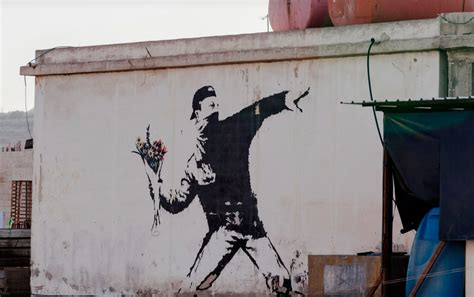
\includegraphics[width=\linewidth,height=.43\textheight,keepaspectratio]{assets/1789622824-banksy_flower.png}\end{center}

\section*{Establishing meaning}

\begin{itemize}
\item Read until line 17 and establish meaning in the text by deciding:

\begin{enumerate}
\item Who is speaking?
\item Who else is there?
\item Where is the speaking/writing taking place?
\item What is the subject of the writing
\item Who is the audience?
\item Why is he writing?
\item What is your first impression of the writer?
\end{enumerate}

\end{itemize}

\section*{Reading}

\section*{Prediction}

\begin{itemize}
\item From what you have read now, what do you think has happened to Joey and the place he lives in? Will he get the ham? Write down you prediction and share it with another student.
\end{itemize}

\section*{Group work}

\begin{itemize}
\item To what extent did your predictions come true?
\item Write down notes on the other half of the questions
\end{itemize}

\section*{Focus}

\begin{center}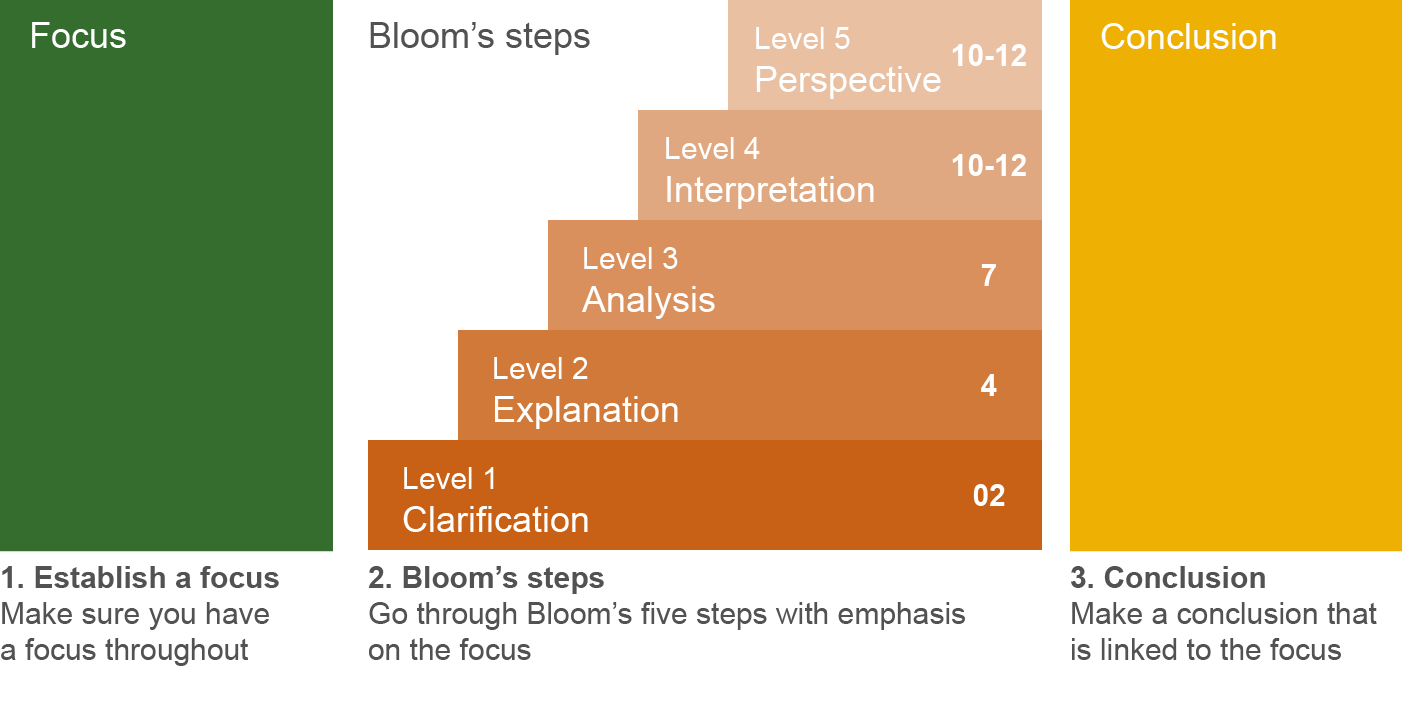
\includegraphics[width=\linewidth,height=.43\textheight,keepaspectratio]{assets/1789622678-.png}\end{center}

\section*{Exit ticket}

\begin{itemize}
\item How do you imagine the origin and the potential end of the world? In what ways are your views reflected in the story?
\end{itemize}

\section*{Materials}

\begin{itemize}
\item How th'Irth Wint Rong
\item \hyperref[worksheet-11]{Worksheet (p.~\pageref*{worksheet-11})}
\end{itemize}

\clearpage\markboth{The Doll's House}{}
\phantomsection\addcontentsline{toc}{section}{3. The Doll's House}
{\color{blue}\small LESSON 03 \hfill 21 September 2026\par}
\vspace{4mm}
{\displayfont\color{navy}\fontsize{30}{34}\selectfont The Doll's House\par}\vspace{4mm}

\section*{Program}

\begin{itemize}
\item \emph{12.05} Vocabulary
\item \emph{12.20} Reading
\item \emph{12.50} Break
\item \emph{13.00} Characterisation and POV
\item \emph{13.15} Reading - continued
\item \emph{13.45} Break
\item \emph{14.00} Creative writing
\end{itemize}

\section*{Vocabulary}

\begin{itemize}
\item Do exercise 1 and 2 on the handout
\end{itemize}

\section*{Reading}

\begin{itemize}
\item Read the very first lines of the story from the beginning as far as and including “… part of the newness.” (lines 1-15). As you read, notice which senses the description appeals to (vision, hearing, smell, taste, touch).
\item In the same part of the text, note who is experiencing the doll’s house: how many experiences are we introduced to, and how can you see the changes in the text?
\item Read the first part of the story (until "... there was nothing more for them to hear" line 107). Make a list of the characters. Write an adjective or a sentence to describe each of them.
\end{itemize}

\section*{Creative writing}
This short story was written in 1922 and describes a middle-class society with middle-class values. Write a short short story of around 2-300 words in which the conflict of the story is transported into the 21st century.


\begin{itemize}
\item The story should have at least three characters.
\item The setting and context must be specific.
\item There should be a clear beginning, middle and end.
\item The story must include at least seven adjectives and NOT ‘good’, ‘bad’, ‘nice’, ‘old’, ‘new’, ‘young’ or ‘normal’
\end{itemize}

\section*{Reading - continued}

\begin{itemize}
\item Do exercise 3 on the handout
\end{itemize}

\section*{Materials}

\begin{itemize}
\item The Doll's House
\item \hyperref[worksheet-12]{The Doll's House - worksheet (p.~\pageref*{worksheet-12})}
\end{itemize}

\clearpage\markboth{Voice in speech}{}
\phantomsection\addcontentsline{toc}{section}{4. Voice in speech}
{\color{blue}\small LESSON 04 \hfill 24 September 2026\par}
\vspace{4mm}
{\displayfont\color{navy}\fontsize{30}{34}\selectfont Voice in speech\par}\vspace{4mm}

\section*{Program}

\begin{itemize}
\item \emph{08.35} Crossword puzzles
\item \emph{09.05} The Rhetorical Situation
\item \emph{09.35} Break
\item \emph{09.50} Speech-making
\item \emph{10.20} Speech-reading
\item \emph{10.40} Break
\item \emph{10.50} Rhetorical analysis
\end{itemize}

\section*{The Rhetorical Situation}

\begin{itemize}
\item \emph{Exigence} What is the (real) purpose of the text? What is the speaker/writer trying to achieve/change? A situation becomes rhetorical once you believe that you can change something in life by uttering something.
\item \emph{Audience} Who is the text meant for? What is the medium, and who is the specific audience of this medium? What is their social background, political and religious belief, age, nationality, gender, ethnicity, etc.? The will be the \emph{mediators of change} who can act on the exigence (i.e. do something about the issue).
\item \emph{Constraints} The rhetorical situation will have som limitations and possibilities related to the context, the speaker/writer, and the mediators of change. These are the constraints. To make a change as likely as possible, what can then be said? What can not?
\end{itemize}

\section*{Apologies}

\par\noindent\textbf{Video:} Video: "My behavior was unacceptable." Will Smith addresses Oscars slap, apologizes to Chris Rock\par\medskip

\section*{Speech-making}

\begin{enumerate}
\item Find information about the United Nations
\item Find information about what happened in Christchurch on the 15th of March 2019.
\end{enumerate}

\begin{itemize}
\item Work in pairs and prepare a speech which lasts two minutes and which includes the most important aspects of the information you found.
\end{itemize}

\section*{Rhetorical analysis}

\begin{itemize}
\item What is the \emph{purpose} of this speech?
\item Who are the \emph{mediators of change}?
\item If change is to happen, how should Jacinda Adern speak? What should she avoid?
\item Find four quotations that you found interesting and reflect on why they caught your attention.
\end{itemize}

\section*{Materials}
\hyperref[worksheet-13]{Crossword puzzle (p.~\pageref*{worksheet-13})}Jacinda Adern: UN speech


\clearpage\markboth{Voice in speech II}{}
\phantomsection\addcontentsline{toc}{section}{5. Voice in speech II}
{\color{blue}\small LESSON 05 \hfill 28 September 2026\par}
\vspace{4mm}
{\displayfont\color{navy}\fontsize{30}{34}\selectfont Voice in speech II\par}\vspace{4mm}

\section*{Program}

\begin{itemize}
\item \emph{12.05} Ardern and Trump
\item \emph{12.15} Rhetorical tools

\begin{itemize}
\item Devices
\item Modes of appeal
\end{itemize}

\item \emph{12.25} Rhetorical tools: analysis
\item \emph{12.50} Break
\item \emph{13.05} Grammatik: Substantiver
\item \emph{13.50} Break
\item \emph{14.00} Pronunciation
\end{itemize}

\section*{Ardern and Trump}

\par\noindent\textbf{Video:} Contrasting styles: Trump and Ardern speak at the UN\par\medskip

\begin{itemize}
\item Describe the differences between the way they speak
\end{itemize}

\section*{Rhetorical tools}

\begin{itemize}
\item "She speaks in a calm, friendly and respectful way."
\item "She uses “we,” “us” and “our” to include everyone"
\item "She gives examples of things like oil spills and nuclear accidents to show how countries affect each other."
\item "She should speak with empathy and responsibility"
\item "She should avoid racism, fear and division."
\end{itemize}

\section*{Devices}

\begin{itemize}
\item alliteˈration: the repetition of a consonant sound at the beginning of words which are close together
\item aˈnaphora: the repetition of one or more words at the beginning of successive clauses
\item anˈtithesis: the placing together of opposing words or ideas to show a contrast
\item ˈassonance: the repetition of vowel sounds in words which are close together
\item ˈmetaphor: an image described by a word or phrase with a concrete meaning but used figuratively
\item personifiˈcation: language in which an inanimate object or concept is spoken of as if it had human life
\item repetition
\item ˈsimile: a figure of speech in which two unlike things are compared using ‘like’ or ‘as’
\item the list of three: three things are listed immediately after each other.
\item inclusive language: language that addresses or includes the audience, often using pronouns such as ‘we’, ‘us’, and ‘our’
\end{itemize}

\section*{Modes of appeal}

\begin{itemize}
\item pathos: an appeal to the audience’s emotions using emotional language, passion and a personal angle
\item logos: an appeal to reason with arguments, evidence, facts and logical reasoning
\item ethos: an appeal to the audience’s trust by sounding eloquent, or by establishing authority or expertise on the subject.
\end{itemize}
\textbf{Example} "Trump uses antithesis when he says that America rejects globalism and embraces patriotism. This device is used to make a pathos appeal to patriotic feelings, which targets American voters and citizens, who can mediate political change by supporting his nationalist policies and voting for leaders who put America first."


\section*{Rhetorical tools: analysis}

\begin{itemize}
\item Find 2-3 examples of rhetorical devices in Jacinda Ardern's speech. Write down the quote and name the device
\item For each example, explain which appeal it supports: ethos, pathos or logos. Then explain how the device and appeal help Ardern achieve the purpose of her speech.
\end{itemize}

\section*{Grammatik: Substantiver}

\section*{Regelmæssige}

{\small\setlength{\tabcolsep}{4pt}\renewcommand{\arraystretch}{1.3}\begin{tabularx}{\linewidth}{@{}>{\raggedright\arraybackslash}X>{\raggedright\arraybackslash}X>{\raggedright\arraybackslash}X@{}}\toprule
Regel & Singularis & Pluralis\\
Substantiver, der i \textbf{singularis} ender på en hvislelyd (en s-agtig lyd), får tilføjet \textbf{-es} i \textbf{pluralis}. & \emph{glass}\newline{}\emph{dish}\newline{}\emph{box} & \emph{glasses}\newline{}\emph{dishes}\newline{}\emph{boxes}\\
Substantiver, der ender på \textbf{-y} efter en konsonant, får tilføjet \textbf{-ies} i \textbf{pluralis}. & \emph{family}\newline{}\emph{baby}\newline{}\emph{sky} & \emph{families}\newline{}\emph{babies}\newline{}\emph{skies}\\
Nogle substantiver, der ender på \textbf{-o}, tilføjer \textbf{-es} i \textbf{pluralis}. & \emph{potato}\newline{}\emph{hero}\newline{}\emph{tomato} & \emph{potatoes}\newline{}\emph{heroes}\newline{}\emph{tomatoes}\\
Nogle substantiver, der ender på \textbf{-f/-fe}, ændres til \textbf{-ves} i \textbf{pluralis}. & \emph{knife}\newline{}\emph{half}\newline{}\emph{wife} & \emph{knives}\newline{}\emph{halves}\newline{}\emph{wives}\\
\bottomrule\end{tabularx}}\par\medskip

\section*{Uregelmæssige}

{\small\setlength{\tabcolsep}{4pt}\renewcommand{\arraystretch}{1.3}\begin{tabularx}{\linewidth}{@{}>{\raggedright\arraybackslash}X>{\raggedright\arraybackslash}X>{\raggedright\arraybackslash}X@{}}\toprule
Regel & Singularis & Pluralis\\
Ved nogle substantiver ændres vokalen. & \emph{man}\newline{}\emph{foot}\newline{}\emph{mouse} & \emph{men}\newline{}\emph{feet}\newline{}\emph{mice}\\
Nogle substantiver tager endelsen \textbf{-en}. & \emph{child}\newline{}\emph{ox} & \emph{children}\newline{}\emph{oxen}\\
Nogle substantiver har samme form i \textbf{singularis} og \textbf{pluralis}. & \emph{sheep}\newline{}\emph{deer}\newline{}\emph{series} & \emph{sheep}\newline{}\emph{deer}\newline{}\emph{series}\\
Nogle substantiver, der er låneord, beholder latinsk/græsk \textbf{pluralisendelse}. & \emph{hypothesis}\newline{}\emph{phenomenon}\newline{}\emph{cactus} & \emph{hypotheses}\newline{}\emph{phenomena}\newline{}\emph{cacti}\\
\bottomrule\end{tabularx}}\par\medskip

\section*{Øvelser}

\begin{enumerate}
\item Lav lektie på minlæring.dk
\item Find substantiver i Jacinda Ardern teksten, og markér om de står i singularis eller pluralis
\end{enumerate}

\section*{Pronunciation}

\begin{enumerate}
\item Listen to the video of Ardern and Trump again, and pick one excerpt - from either Ardern or Trump - that you would like to try an imitate. Listen to that excerpt carefully, sentence by sentence, and notice how the speaker stresses each word in the sentence.
\item When you are ready, individually record your perfect reading/imitation of the paragraph. Use e.g. \href{https://wavacity.com/}{Audacity}
\item Listen to your recording back to back with the audiobook and notice any deviations.
\item Practise deviations found in 3. and re-record your reading.
\end{enumerate}

\section*{Materials}

\begin{itemize}
\item Jacinda Ardern: Speech
\item Ardern and Trump
\end{itemize}

\clearpage\markboth{The King's Speech}{}
\phantomsection\addcontentsline{toc}{section}{6. The King's Speech}
{\color{blue}\small LESSON 06 \hfill 5 October 2026\par}
\vspace{4mm}
{\displayfont\color{navy}\fontsize{30}{34}\selectfont The King's Speech\par}\vspace{4mm}

\section*{Program}

\begin{itemize}
\item \emph{12.05} Warm up
\item \emph{12.15} The King's Speech
\end{itemize}

\section*{Warm up}

\begin{itemize}
\item Stephen Fry, \emph{Have you heard of Oscar Wilde?}
\item Greogory Maguire, \emph{How th'Irth Wint Rong by Hapless Joey@homeskool.guv}
\item Katherine Mansfield, \emph{The Doll's House}
\item Jacinda Ardern, \emph{Address to the UN General Assembly}
\end{itemize}

\begin{enumerate}
\item For each text, choose one keyword that connects it to the concept of \emph{voice}
\item Choose the two texts that show the most different aspects of voice. Discuss how they connect.
\end{enumerate}

\section*{The King's Speech}

\begin{itemize}
\item Draw a charactersheet from this summary of the film:
\end{itemize}

\noindent\begin{minipage}[c]{.51\linewidth}
After the death of his father King George V (Michael Gambon) and the scandalous abdication of King Edward VIII (Guy Pearce), Bertie (Colin Firth) who has suffered from a debilitating speech impediment all his life, is suddenly crowned King George VI of England.With his country on the brink of war and in desperate need of a leader, his wife, Elizabeth (Helena Bonham Carter), the future Queen Mother, arranges for her husband to see an eccentric speech therapist, Lionel Logue (Geoffrey Rush). After a rough start, the two delve into an unorthodox course of treatment and eventually form an unbreakable bond. With the support of Logue, his family, his government and Winston Churchill (Timothy Spall), the King will overcome his stammer and deliver a radio-address that inspires his people and unites them in battle. Based on the true story of King George VI,THE KING'S SPEECH follows the Royal Monarch's quest to find his voice.

\end{minipage}\hfill\begin{minipage}[c]{.44\linewidth}\centering
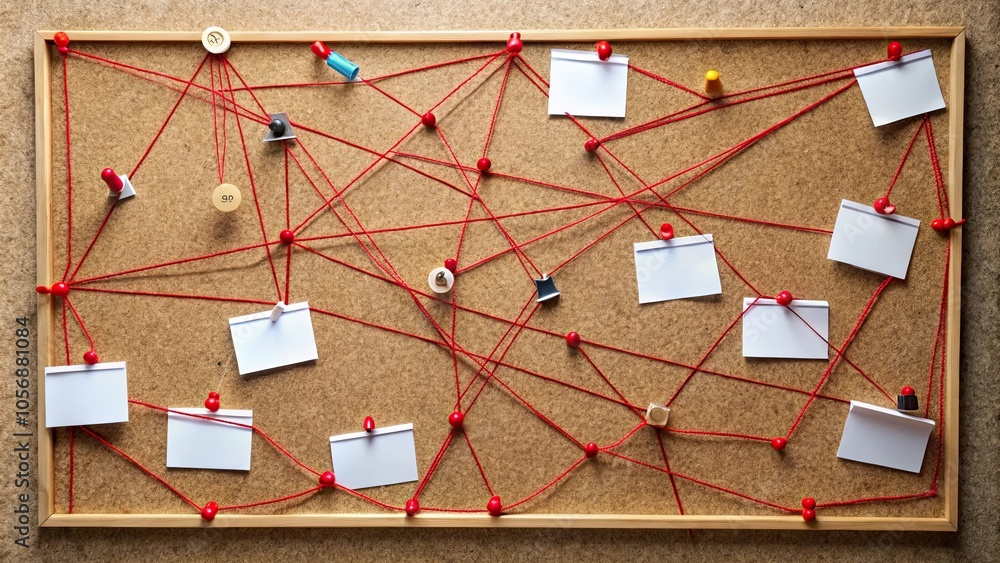
\includegraphics[width=\linewidth,height=.4\textheight,keepaspectratio]{assets/1791190927-suspect.png}\end{minipage}\par\medskip

\clearpage\markboth{Voices}{}
\phantomsection\addcontentsline{toc}{section}{7. Voices}
{\color{blue}\small LESSON 07 \hfill 8 October 2026\par}
\vspace{4mm}
{\displayfont\color{navy}\fontsize{30}{34}\selectfont Voices\par}\vspace{4mm}

\section*{Program}

\begin{itemize}
\item \emph{08.35} The King's Speech
\item \emph{08.45} Quick write
\item \emph{08.50} The Rhetorical Situation
\item \emph{09.50} Break
\item \emph{10.05} Codenames
\end{itemize}

\section*{The King's Speech}

\begin{itemize}
\item What aspect of voice did The King's Speech add to the theme? Choose 5 keywords
\end{itemize}

\begin{center}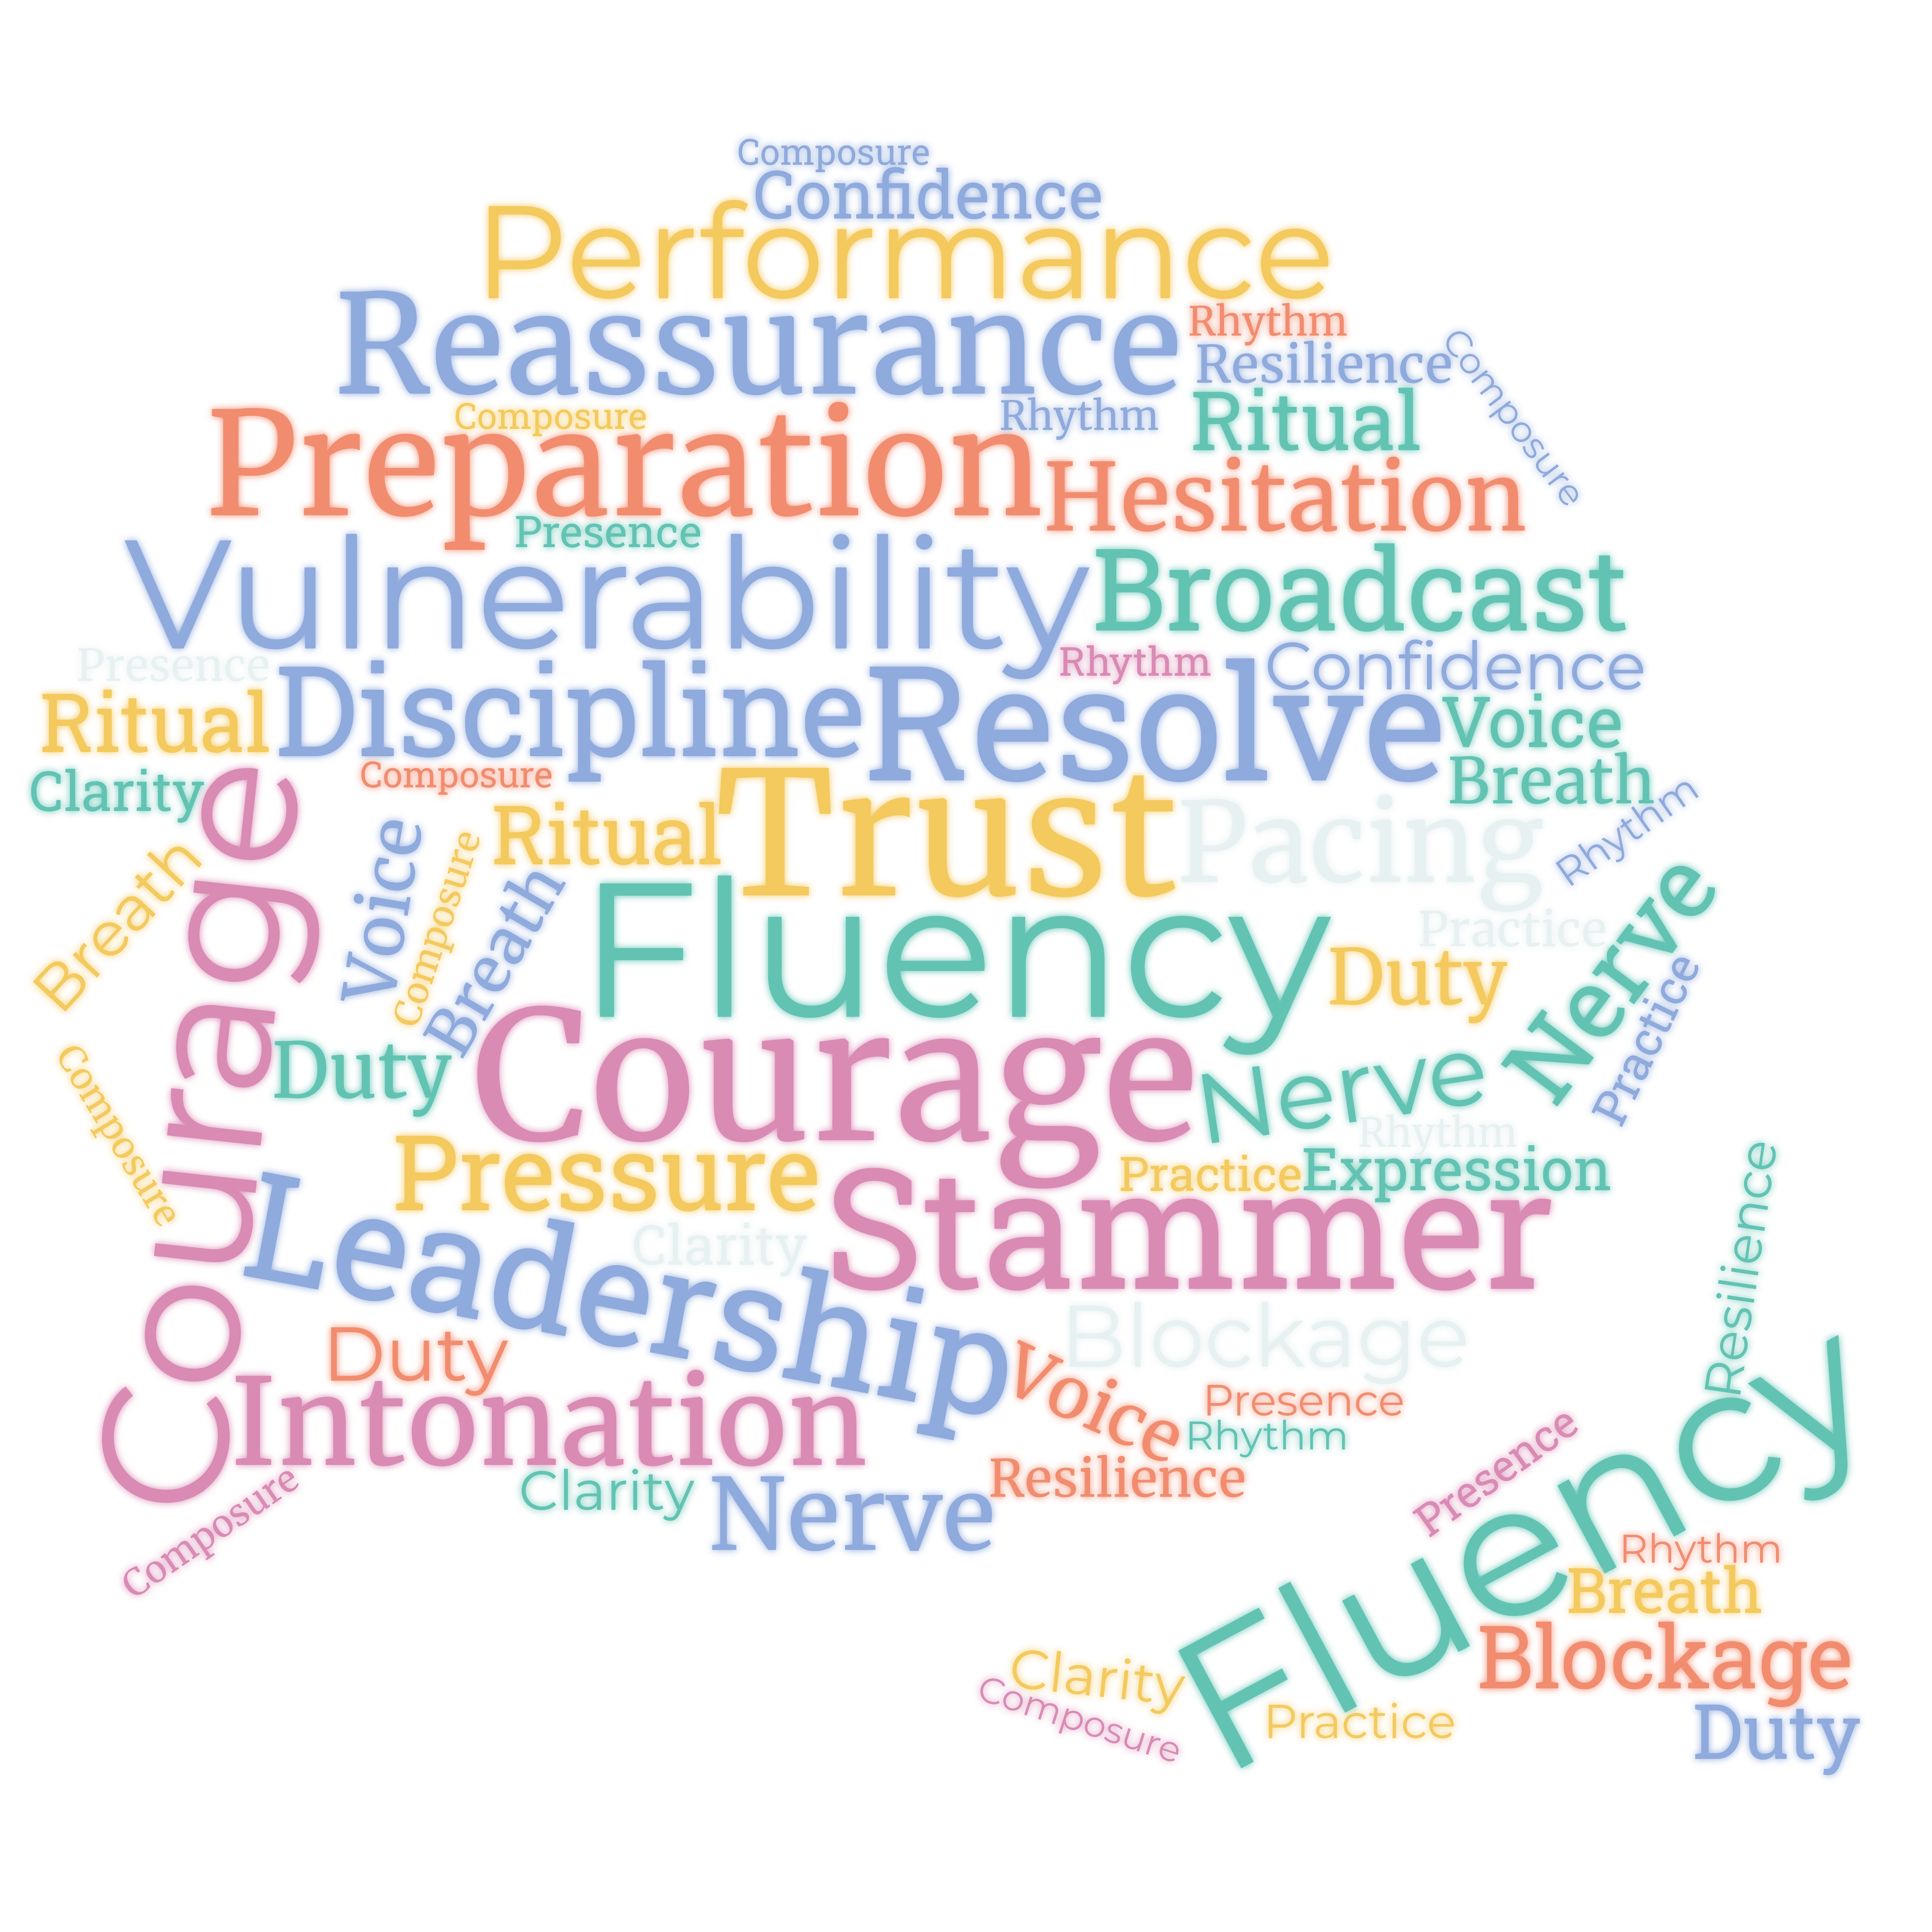
\includegraphics[width=\linewidth,height=.43\textheight,keepaspectratio]{assets/wordcloud.png}\end{center}

\section*{Quick write}

\begin{itemize}
\item Write for 5 minutes about the connection between the film and at least one of the other texts. Use at least 5 words from the whiteboard in your writing.

\begin{itemize}
\item Stephen Fry, \emph{Have you heard of Oscar Wilde?}
\item Greogory Maguire, \emph{How th'Irth Wint Rong by Hapless Joey@homeskool.guv}
\item Katherine Mansfield, \emph{The Doll's House}
\item Jacinda Ardern, \emph{Address to the UN General Assembly}
\item \emph{The King's Speech}
\end{itemize}

\end{itemize}

\section*{Rhetorical situation}

\par\noindent\textbf{Video:} The King to His Peoples. H.M. King George VI from Buckingham Palace September 3rd 1939\par\medskip

\begin{itemize}
\item Write a description of the rhetorical situation around the king's speech. Each category should be described by at least 75 words. Use questions on the handout to guide your descriptions, but write your descriptions in your own voice.
\end{itemize}

\section*{Materials}

\begin{itemize}
\item \hyperref[worksheet-14]{The Rhetorical Situation: handout (p.~\pageref*{worksheet-14})}
\end{itemize}

\clearpage\phantomsection\addcontentsline{toc}{chapter}{3. The Future Is Written}\markboth{The Future Is Written}{}\thispagestyle{empty}
\fancyhead[L]{\small\color{blue}The Future Is Written}
\vspace*{12mm}
{\color{blue}\large CHAPTER 3\par}\vspace{8mm}
{\displayfont\color{navy}\fontsize{43}{47}\selectfont The Future Is Written\par}\vspace{12mm}
\begin{center}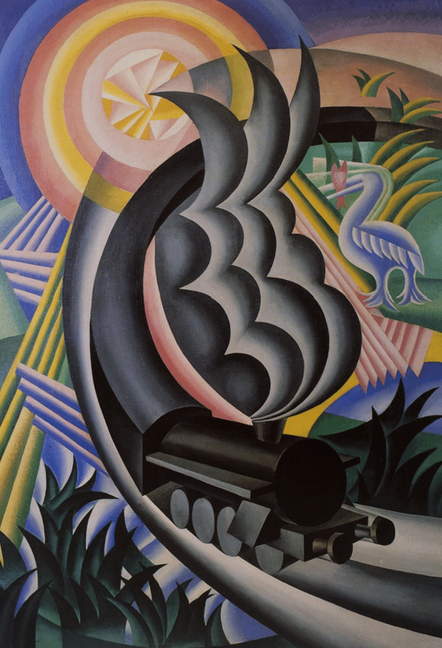
\includegraphics[width=\linewidth,height=.48\textheight,keepaspectratio]{assets/Sci-fi-train.png}\end{center}\vfill
{\large Science fiction, memory, artificial intelligence, human relationships, and visions of space exploration.\par}\clearpage

\clearpage\markboth{Brave New World}{}
\phantomsection\addcontentsline{toc}{section}{1. Brave New World}
{\color{blue}\small LESSON 01 \hfill 19 October 2026\par}
\vspace{4mm}
{\displayfont\color{navy}\fontsize{30}{34}\selectfont Brave New World\par}\vspace{4mm}

\section*{Program}

\begin{itemize}
\item \emph{12.05} Warm up
\item \emph{12.15} Utopias and dystopias
\item \emph{12.45} Break
\item \emph{13.00} Types of sci-fi
\item \emph{13.15} Brave New World
\item \emph{14.00} Break
\item \emph{14.10} Reading
\end{itemize}

\section*{Warm up}
\begin{quotebox}
people will come to love their oppression, adore the technologies that undo their capacities to think.

— Aldous Huxley

\end{quotebox}
\begin{taskbox}
\tasktitle{Discuss with your classmates}
\begin{enumerate}
\item Are you mainly optimistic or pessimistic about the future?
\item What role does technology/science play in your vision of the future?
\item Discuss Aldous Huxley’s quote above. To what extent do you agree/disagree?
\end{enumerate}
\end{taskbox}

\section*{Utopias and dystopias}
As the thought experiments above indicate, there are basically two kinds of science fiction: utopian and dystopian. The word 'utopia' was coined by the British writer Thomas More in 1516. Utopia, meaning 'good place',was the title of his book which outlined a perfect, flawless and harmonious society without any greed, corruption or power struggles due to the fact that there was no private property. The opposite of a utopia is dystopia. Like 'utopia', the word has Greek roots and simply means 'bad place', in other words a worst-case scenario of how a society might turn out.


\begin{itemize}
\item \emph{Topos}: Greek for “place”.
\item \emph{Ou}: Greek for “not” or “no”.
\item \emph{Eu}: Greek for “good” or “well”.
\item \emph{Dys}: Greek for “bad” or “difficult”.
\end{itemize}
\begin{taskbox}
\tasktitle{Draw in pairs}
\begin{enumerate}
\item Instruct your classmate to draw a place that you think could be called u-/dystopia.
\end{enumerate}
\end{taskbox}

\section*{Types of sci-fi}
Earlier, we learned that there are basically two kinds of science fiction: utopian and dystopian. There are, however, also a few other sets of pairs that might help us understand what sci-fi is. The first one is that there are sci-fi stories set in outer space, commonly known as ‘space operas’, as well as sci-fi stories set on Earth in a more or less distant future, for instance Brave New World and Nineteen Eighty-Four that we mentioned above. Space opera with aliens, spaceships, galactic wars, cyborgs and so on is perhaps the least respected of the sub-genres of science fiction, but also one of the most popular and certainly what most people associate with science fiction.

Secondly, there are also two kinds of sci-fi stories in the sense that there is ‘hard science fiction’ and ‘soft science fiction’. Soft science fiction is used to describe stories that focus on the human element rather than scientific facts and technical details. Hard SF, on the other hand, is the most science-oriented category and focuses on facts. Hard SF is also more likely to use the language of science directly. Since this type of SF sticks to facts, it usually explores what already exists, i.e. the perspectives already opened up by contemporary science and technology. However, the boundaries between the two kinds might be blurred and to some extent the categories are marketing terms used to target different groups of readers.


{\small\setlength{\tabcolsep}{4pt}\renewcommand{\arraystretch}{1.3}\begin{tabularx}{\linewidth}{@{}>{\raggedright\arraybackslash}X>{\raggedright\arraybackslash}X@{}}\toprule
Types - in terms of opposites & \\
utopian & dystopian\\
space stories, incl. space operas & future on earth stories\\
hard sci-fi & soft sci-fi\\
near future & far future\\
\bottomrule\end{tabularx}}\par\medskip
\begin{taskbox}
\tasktitle{Discuss}
\begin{enumerate}
\item Have you read or watched stories that fit either of the categories?
\end{enumerate}
\end{taskbox}

\section*{Brave New World}

\noindent\begin{minipage}[c]{.51\linewidth}
\begin{quote}\tasktitle{Work with the text}

\begin{enumerate}
\item Do the exercises on the handout.
\item Read the first chapter of Brave New World
\end{enumerate}
\end{quote}
\end{minipage}\hfill\begin{minipage}[c]{.44\linewidth}\centering
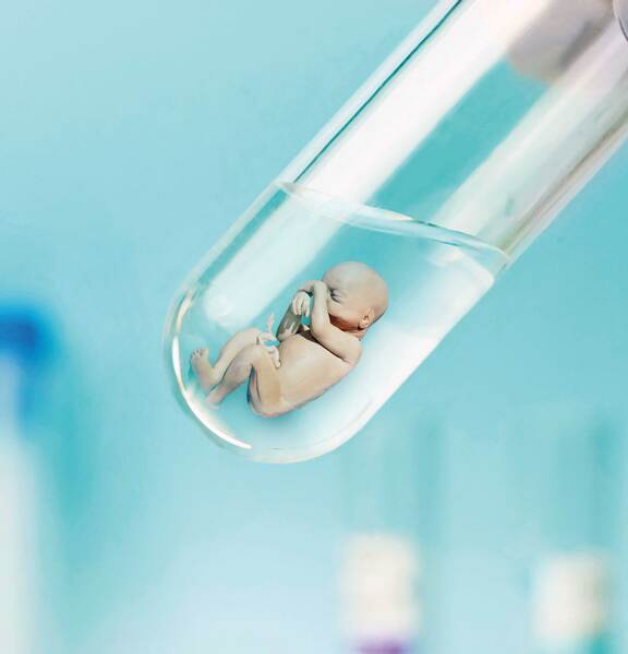
\includegraphics[width=\linewidth,height=.4\textheight,keepaspectratio]{assets/1792400829-bnw.png}\end{minipage}\par\medskip

\section*{Materials}

\begin{itemize}
\item \hyperref[worksheet-15]{Brave New World: Worksheet (p.~\pageref*{worksheet-15})}
\item Brave New World: Excerpt
\end{itemize}

\clearpage\markboth{Brave New World II}{}
\phantomsection\addcontentsline{toc}{section}{2. Brave New World II}
{\color{blue}\small LESSON 02 \hfill 22 October 2026\par}
\vspace{4mm}
{\displayfont\color{navy}\fontsize{30}{34}\selectfont Brave New World II\par}\vspace{4mm}

\section*{Program}

\begin{itemize}
\item \emph{08.35} Warm up / recap
\item \emph{09.05} World building
\item \emph{09.25} Break
\item \emph{09.40} Analysis
\item \emph{10.30} Break
\item \emph{10.40} Adaptation
\end{itemize}

\section*{Warm up / recap}
\begin{taskbox}
\tasktitle{In pairs:}
\begin{enumerate}
\item Make a list of the casts of this society, and the jobs reserved for the members of these casts.
\item One student is an Alpha from the Hatchery, the other an Epsilon. The Alpha student outlines the scientific advances and explain the Bokanovsky process so an Epsilon can understand it, and the Epsilon asks questions for clarification.
\end{enumerate}
\end{taskbox}
\begin{taskbox}
\tasktitle{Individually:}
\begin{enumerate}
\item Finish reading the first chapter of Brave New World
\item Make a list of the casts of this society, and the jobs reserved for the members of these casts.
\item Write an explanation of the Bokanovsky Process addressed to an Epsilon – simplify the scientific explanation so the Epsilon can understand you but stay true to the facts. Use informal English and be as objective as possible.
\end{enumerate}
\end{taskbox}

\section*{World building}
\begin{quotebox}
A squat grey building of only thirty-four stories. Over the main entrance the words, CENTRAL LONDON HATCHERY AND CONDITIONING CENTRE, and, in a shield, the World State’s motto, COMMUNITY, IDENTITY, STABILITY.

\end{quotebox}
In science fiction, the setting is often a character in itself. The above quote is however the only description of the outside world we get in the first chapter. What we get instead is a description of how society is structured. Can we use this to imagine how such a society might look?

\begin{taskbox}
\tasktitle{Create}
\begin{enumerate}
\item In the form of a poster (it may be digital), or a literary discription, make a depiction of the outside world of Brave New World.
\item Find five quotes that inspired your choices.
\end{enumerate}
\end{taskbox}

\section*{Analysis}
\begin{taskbox}
\tasktitle{Work with the text}
\begin{enumerate}
\item Discuss answers to the questions on the handout. Write down notes to your answers.
\end{enumerate}
\end{taskbox}

\section*{Adaptation}
Watch the first 18 minutes of the tv-show Brave New World and do the reflection exercise below

In the novel, the world state motto is "Community, Identity, Stability", in the show New London has three rules: "No privacy. No family. No monogamy".

\begin{taskbox}
\tasktitle{Reflect}
\begin{enumerate}
\item Write for 5 minutes about the the show's interpretation of the brave new world of the novel. Did the world look like you had imagined it? What's the connection between the New London rules and the World State motto?
\end{enumerate}
\end{taskbox}

\section*{Glossary}

\begin{itemize}
\item \textbf{Cognitive estrangement:} Science fiction makes familiar things seem strange so we can look at our own world in a new way. Its unfamiliar world follows an understandable logic.
\item \textbf{Info-dump:} A passage that gives the reader a large amount of background information about the fictional world at once. This can happen through a narrator’s explanation or a character’s speech, such as the Director’s tour of the Hatchery.
\end{itemize}

\section*{Materials}

\begin{itemize}
\item \hyperref[worksheet-16]{Brave New World: Handout (p.~\pageref*{worksheet-16})}
\item Brave New World: S01E01
\end{itemize}

\clearpage\markboth{The Relive Box}{}
\phantomsection\addcontentsline{toc}{section}{3. The Relive Box}
{\color{blue}\small LESSON 03 \hfill 26 October 2026\par}
\vspace{4mm}
{\displayfont\color{navy}\fontsize{30}{34}\selectfont The Relive Box\par}\vspace{4mm}

\section*{Program}

\begin{itemize}
\item \emph{12.05} Memory
\item \emph{12.25} Reading
\item \emph{12.55} Break
\item \emph{13.10} Reading - cont.
\item \emph{13.40} Formal vs. informal language
\item \emph{14.00} Working with the text
\item \emph{14.30} Summing up
\end{itemize}

\section*{Memory}
\begin{taskbox}
\tasktitle{vocabulary}
\begin{enumerate}
\item The words and expressions below are all related to memory. Look up the ones you are not familiar with.
\end{enumerate}
\emph{recollect – call to mind – a trip down memory lane – fix in the mind – hold dear – dwell on the past – recall – relive – think back – in retrospect – reminiscence – treasure – cherish – have a flashback – ring a bell – anamnesis – dig into the past – backtrace}

\end{taskbox}

\par\medskip{\color{rule}\hrule}\medskip
\begin{taskbox}
\tasktitle{In pairs}
2. How many of the words and expressions from previous slide can you remember?
3. If you had the chance to relive a memory from your past, what would it be and why? Describe the memory, what happens, the mood, the setting etc. You may include some of the words from the list in the previous slide.

\end{taskbox}

\par\medskip{\color{rule}\hrule}\medskip

\par\noindent\textbf{Video:} Spatial Scene is INSANE (Apple Vision Pro, visionOS 26)\par\medskip

\section*{Reading}

\noindent\begin{minipage}[c]{.51\linewidth}

\begin{enumerate}
\item Read the short story, focusing on: What is a Relive Box and how does it work according to the story? Note down keywords. Make a list of pros and cons about the Relive Box as they come across in the story, directly or indirectly.
\end{enumerate}
\end{minipage}\hfill\begin{minipage}[c]{.44\linewidth}\centering

\includegraphics[width=\linewidth,height=.4\textheight,keepaspectratio]{assets/1793003299-reading.png}\end{minipage}\par\medskip

\section*{Formal vs. informal language}
\begin{taskbox}
\tasktitle{In pairs or individually}
\begin{enumerate}
\item Using your notes from your reading focus, write a short but instructive manual for the second-generation Halcom XI520 Relive Box (100-200 words). Use formal language.
\item Now write an unofficial manual for the internet using informal language (50-100 words). It is a manual for people who found it hard to understand the official manual that you wrote in the previous exercise.
\end{enumerate}
\end{taskbox}

\section*{Working with the text}
\begin{taskbox}
\tasktitle{Analysis}
\begin{enumerate}
\item Work with the questions on the handout. Start with your assigned questions.
\item Be prepared to present your answer.
\end{enumerate}
\end{taskbox}

\section*{Materials}

\begin{itemize}
\item The Relive Box: Short story
\item \hyperref[worksheet-17]{The Relive Box: Worksheet (p.~\pageref*{worksheet-17})}
\end{itemize}

\clearpage\markboth{Tell Me an Ending}{}
\phantomsection\addcontentsline{toc}{section}{4. Tell Me an Ending}
{\color{blue}\small LESSON 04 \hfill 5 November 2026\par}
\vspace{4mm}
{\displayfont\color{navy}\fontsize{30}{34}\selectfont Tell Me an Ending\par}\vspace{4mm}

\section*{Program}

\begin{itemize}
\item \emph{08.35} Summing up The Relive Box
\item \emph{09.00} Read Tell me an ending untill end of page 11
\item \emph{09.30} Working with the text: part 1
\item \emph{09.45} Break
\item \emph{10.00} Read the rest of the story
\item \emph{10.30} Working with the text: part 2
\item \emph{11:05} Sum up
\end{itemize}

\section*{Summing up The Relive Box}
\begin{taskbox}
\tasktitle{Categorise}
\begin{enumerate}
\item Look at your notes on your assigned questions from last lesson: Put your questions into one of the categories on the whiteboard.
\item Write down the letter of your questions as well as keywords connected to that question under the category on the whiteboard.
\end{enumerate}
\end{taskbox}

\section*{Working with the text: part 1}
\begin{taskbox}
\tasktitle{Quick write}
\begin{enumerate}
\item Write an entry for an encyclopedia like Wikipedia on Nepenthe’s method of memory removal (100-200 words). Use formal and objective language and include the following terms: self-informed, self-confidential, the company name Nepenthe, traces and restoration. You can mimic this wiki site on ECT.
Make sure to include the backstory and development of the scientific procedure.
\end{enumerate}
\end{taskbox}

\section*{Working with the text: part 2}
\begin{taskbox}
\tasktitle{In groups}
\begin{enumerate}
\item Record a ten minute, non-scripted conversation about the text and listen to it afterwards, OR
\item Make a poster that visually presents the themes of the novel excerpt, and connects it to Brave New World and The Relive Box, and possibly one other text. It should show how the texts connect, not just that they connect, OR
\item Mimicking the questions from last lesson, come up with 5 questions about the text. Discuss and answer the questions, AND
\item Make a summary of your work to present to class
\end{enumerate}
\end{taskbox}
\begin{taskbox}
\tasktitle{Individually}
\begin{enumerate}
\item Prepare an oral presentation of the text with at least 5 bullets. Rehearse the presentation (no reading aloud), and make sure you can talk for 6 minutes, OR
\item Make a poster that visually presents the themes of the novel excerpt, and connects it to Brave New World and The Relive Box, and possibly one other text. It should show how the texts connect, not just that they connect, OR,
\item Mimicking the questions from last lesson, come up with 5 questions about the text. Answer the questions, AND
\item Make a summary of your work to present to class
\end{enumerate}
\end{taskbox}

\section*{Materials}

\begin{itemize}
\item Tell Me an Ending
\end{itemize}

\clearpage\markboth{Be Right Back}{}
\phantomsection\addcontentsline{toc}{section}{5. Be Right Back}
{\color{blue}\small LESSON 05 \hfill 9 November 2026\par}
\vspace{4mm}
{\displayfont\color{navy}\fontsize{30}{34}\selectfont Be Right Back\par}\vspace{4mm}

\section*{Program}

\begin{itemize}
\item \emph{12.05} Warm up
\item \emph{12.15} Can AI 'cure' grief?
\item \emph{12.30} Be Right Back
\item \emph{13.20} Break
\item \emph{13.35} Working with the text
\item \emph{14.20} Break
\item \emph{14.30} Written assignment
\end{itemize}

\section*{Warm up}
\begin{taskbox}
\tasktitle{Discuss}
\begin{enumerate}
\item Look up information on ‘the empty chair’ technique used in psychotherapy. Why and how is it used?
\item Discuss with your neighbour whom you would place in ‘the empty chair’, what you would ask them and why.
\end{enumerate}
\end{taskbox}

\section*{Can AI 'cure' grief?}

\par\noindent\textbf{Video:} Can AI ’cure’ grief? - BBC\par\medskip

\section*{Be Right Back}

\begin{center}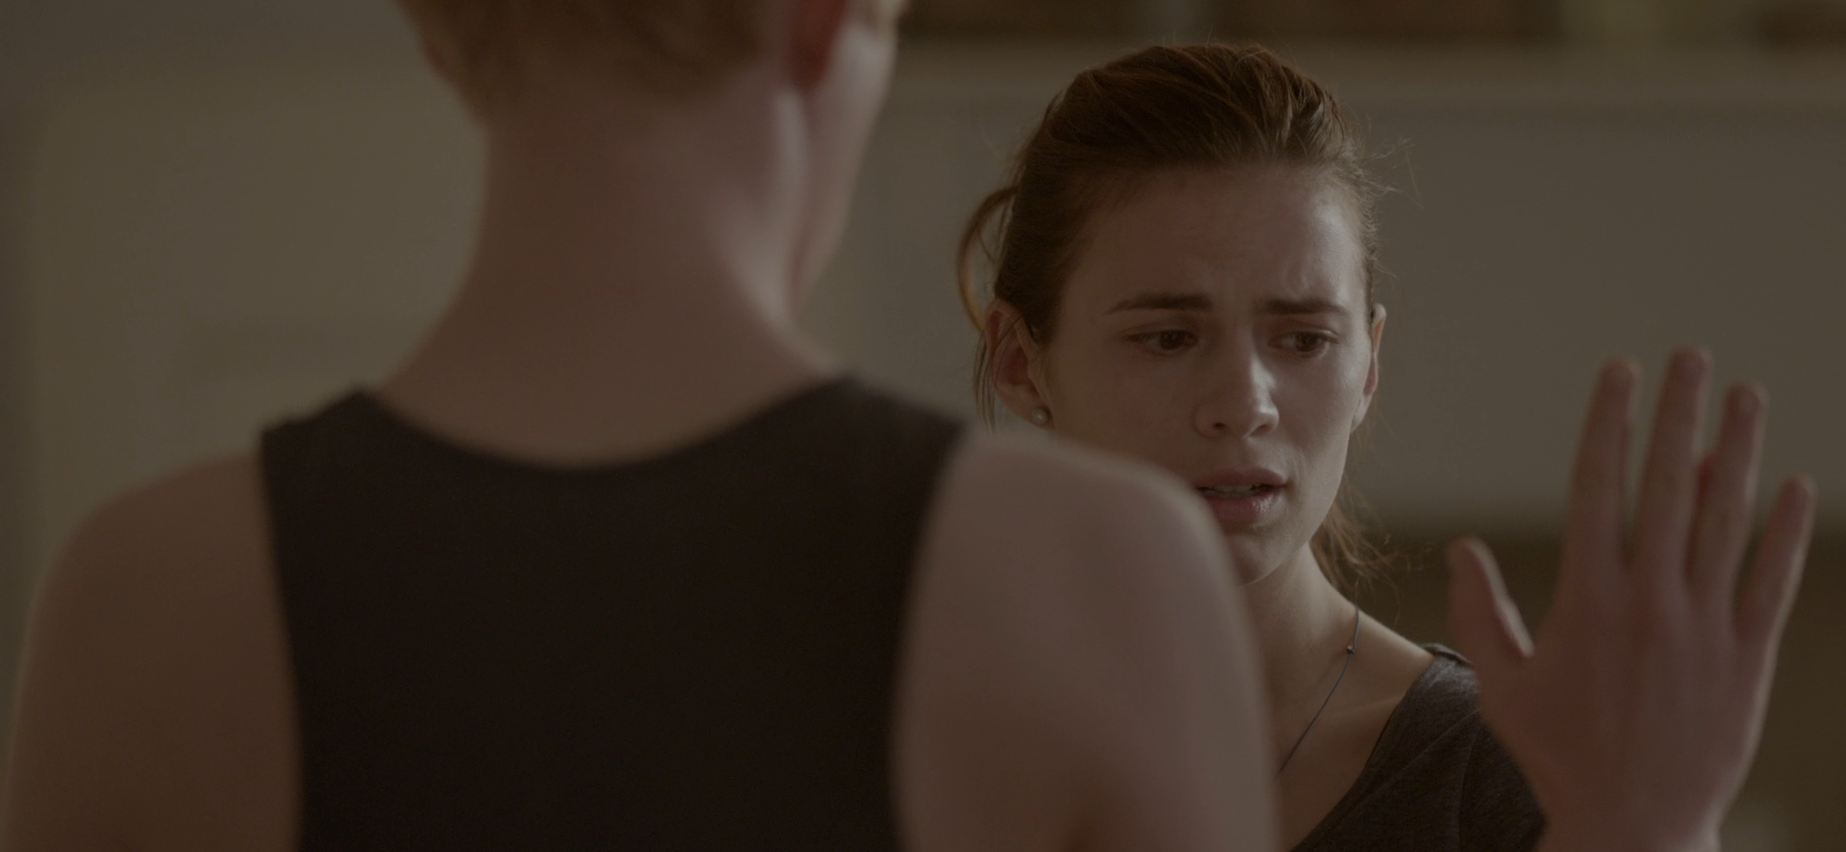
\includegraphics[width=\linewidth,height=.43\textheight,keepaspectratio]{assets/berightback.png}\end{center}
\begin{taskbox}
\tasktitle{Watch}
\begin{enumerate}
\item Watch the episode "Be Right Back" from season 2 of the tv-show Black Mirror
\end{enumerate}
\end{taskbox}

\section*{Working with the text}
\begin{taskbox}
\tasktitle{Create}
\begin{enumerate}
\item In groups, select and analyse a scene from the film that you particularly liked, found important or were intrigued by. In your analysis, you must include a focus on filmic devices such as close-ups, perspective, sound effects or lighting. Moreover, connect the scene to the episode as a whole and give reasons why you picked this scene. Create a slideshow with stills from the film, that presents your analysis.
\end{enumerate}
\end{taskbox}

\section*{Written assignment}
\begin{taskbox}
\tasktitle{Write}
\begin{enumerate}
\item Read the article "How we feel about robots that feel"
\item Write an e-mail from Martha to the company that produced ‘Ash’. Your letter must try to pinpoint what it is that makes a human-robot relationship like this creepy. Be as specific as possible. You can either argue that the company ought to put an end to production or that the company needs to advertise the robots differently. Use formal language (500 words).
\end{enumerate}
\end{taskbox}

\section*{Materials}

\begin{itemize}
\item Black Mirror, S02E01
\item How We Feel About Robots That Feel
\end{itemize}

\clearpage\markboth{Space Policy}{}
\phantomsection\addcontentsline{toc}{section}{6. Space Policy}
{\color{blue}\small LESSON 06 \hfill 12 November 2026\par}
\vspace{4mm}
{\displayfont\color{navy}\fontsize{30}{34}\selectfont Space Policy\par}\vspace{4mm}

\section*{Program}

\begin{itemize}
\item \emph{08.35} American values
\item \emph{09.00} On US Space Policy
\item \emph{09.40} Break
\item \emph{09.55} Analysis
\item \emph{10.40} Break
\item \emph{10.50} Sum up
\end{itemize}

\section*{American Values}
\begin{taskbox}
\tasktitle{Research}
\begin{enumerate}
\item Look up information on the following concepts and events in American history. Post small descriptions as well as pictures to illustrate them on edaptio.

\begin{itemize}
\item The Lewis and Clark expedition
\item The pioneers/settlers who went west
\item The frontier thesis
\item Manifest Destiny
\end{itemize}

\end{enumerate}
\end{taskbox}

\begin{center}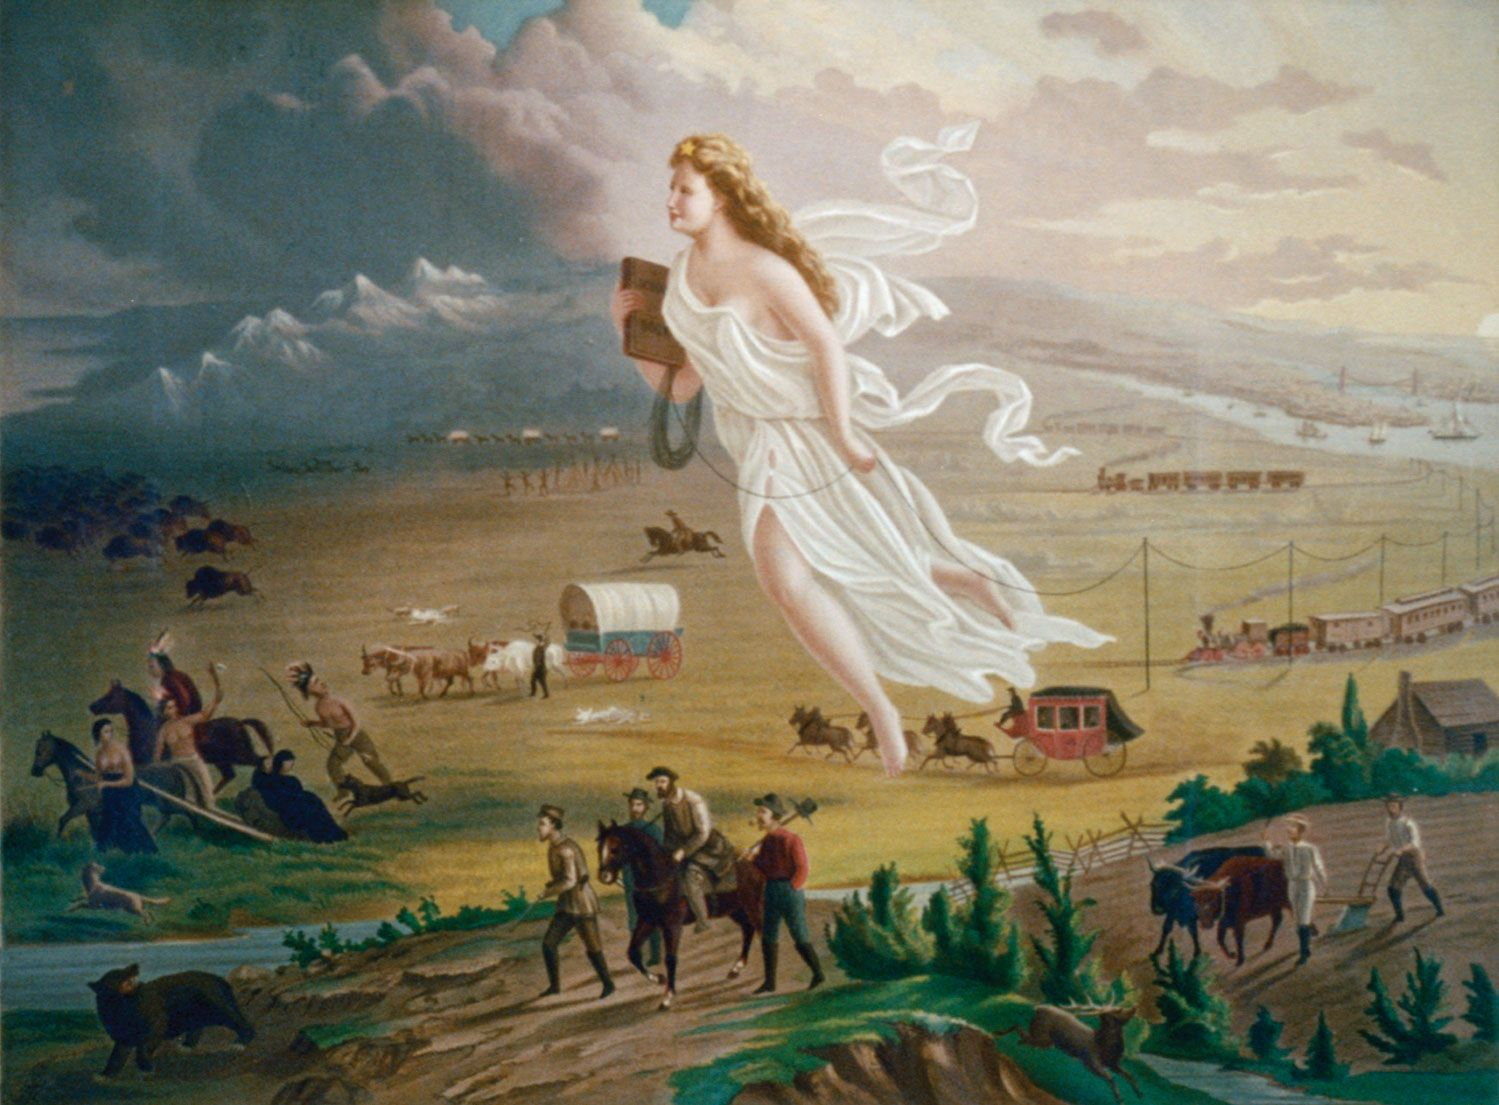
\includegraphics[width=\linewidth,height=.43\textheight,keepaspectratio]{assets/1794426155-manifest.png}\end{center}

\section*{On US Space Policy}
\begin{taskbox}
\tasktitle{Reading focus}
\begin{enumerate}
\item Make notes on the points below and note down the line numbers for the quotes you find interesting and relevant for your focus.

\begin{itemize}
\item Compile a list of rhetorical devices used in the speech.
\item Note down references to American history and values as well as references to mankind in general and international cooperation.
\item Jot down all references to journeys, knowledge and progress.
\item Make a timeline of the milestones proposed by Bush.
\end{itemize}

\end{enumerate}
\end{taskbox}

\section*{Analysis}
\begin{taskbox}
\tasktitle{Discuss}
\begin{enumerate}
\item Discuss answers to questions on hand-out.
\end{enumerate}
\end{taskbox}

\section*{Materials}

\begin{itemize}
\item Remarks on US Space Policy
\item \hyperref[worksheet-18]{Worksheet (p.~\pageref*{worksheet-18})}
\end{itemize}

\clearpage\markboth{Settled In}{}
\phantomsection\addcontentsline{toc}{section}{7. Settled In}
{\color{blue}\small LESSON 07 \hfill 16 November 2026\par}
\vspace{4mm}
{\displayfont\color{navy}\fontsize{30}{34}\selectfont Settled In\par}\vspace{4mm}

\section*{Program}

\begin{itemize}
\item \emph{12.05} Warm up
\item \emph{12.25} Settled In
\item \emph{12.50} Break
\item \emph{13.05} Comprehension
\item \emph{13.20} Analysis
\item \emph{14.10} Break
\item \emph{14.20} Essay-writing
\end{itemize}

\section*{Warm up}

\par\noindent\textbf{Video:} Elon Musk shares 'tentative' Mars game plan in SpaceX update at Starbase\par\medskip
\begin{taskbox}
\tasktitle{Reflect}
\begin{enumerate}
\item Do you think Musk's vision of human civilisation being a spacefaring civilisation is utopian?
\item Do you think humans will colonise Mars in your lifetime? How does this make you feel?
\end{enumerate}
\end{taskbox}

\section*{Settled In}
Tim Dudenhoefer is a systems engineer working for NASA at the NASA Goddard Space Flight Center. He grew up outside of Pittsburgh, Pennsylvania along the shores of the Allegheny River where he learned to love the outdoors, reading, writing, science fiction and engineering. He has been writing stories since he was a child.

In 2026 NASA invited writers of sci-fi to submit stories about future journeys and the possible terraforming of Mars to a competition. NASA turned their attention to science fiction as they believed that it might help them “look beyond predictable outcomes and identify mitigation approaches for previously unforeseen risks.“ Tim Dudenhoefer’s story is one of the winning entries in the competition.

\begin{taskbox}
\tasktitle{Read}
\begin{enumerate}
\item Read the short story Settled In by Tim Dudenhoefer
\end{enumerate}
\end{taskbox}

\section*{Comprehension}
\begin{taskbox}
\tasktitle{Discuss}
\begin{enumerate}
\item Where are we when the story begins, and who are the people there?
\item Where are they headed?
\item Who and what are Percy and Jo?
\item What is Shackleton?
\item Who was the narrator’s father and what happened to him?
\item What has happened in the narrator’s personal life since leaving Earth?
\item What role did A.I. play in the human mission to Mars?
\end{enumerate}
\end{taskbox}

\section*{Analysis}
\begin{taskbox}
\tasktitle{Write}
\begin{enumerate}
\item Choose 5 questions on the hand out. Answer each question in writing (at least 50 words).
\item Collect your answers into one text of 5 paragraphs.
\item Try to make the text as cohesive as possible by adding \href{https://theenglishhandbook.systime.dk/?id=247\#c1764}{linking words}, an introduction, and/or a conclusion.
\end{enumerate}
\end{taskbox}

\section*{Materials}

\begin{itemize}
\item Settled In
\item \hyperref[worksheet-19]{Worksheet (p.~\pageref*{worksheet-19})}
\end{itemize}

\clearpage\markboth{On a Sunbeam}{}
\phantomsection\addcontentsline{toc}{section}{8. On a Sunbeam}
{\color{blue}\small LESSON 08 \hfill 19 November 2026\par}
\vspace{4mm}
{\displayfont\color{navy}\fontsize{30}{34}\selectfont On a Sunbeam\par}\vspace{4mm}

\section*{Program}

\begin{itemize}
\item \emph{08.35} Warm up
\item \emph{08.45} On a Sunbeam
\item \emph{09.15} Break
\item \emph{09.40} Analysis
\item \emph{10.00} Break
\item \emph{10.30} Extra
\end{itemize}

\section*{Warm up}
\begin{taskbox}
\tasktitle{Quick write}
\begin{enumerate}
\item Picture yourself on your back on a lawn at night looking up at the starlit sky. For a minute write down your feelings and thoughts. You might include or find inspiration in some of the words below.

\begin{itemize}
\item vast – fathomless – infinite – alone – insignificant – depth – staggering – indeterminable – unbounded – cosmic – limitless – prodigious – other-worldly – solitude – eternity – ephemeral
\end{itemize}

\end{enumerate}
\end{taskbox}

\begin{center}
\includegraphics[width=\linewidth,height=.43\textheight,keepaspectratio]{assets/1795013794-sky.png}\end{center}



\section*{On a Sunbeam}

\noindent\begin{minipage}[c]{.51\linewidth}
\begin{taskbox}
\tasktitle{Read}
\begin{enumerate}
\item Read the first two (or three) chapters of the webcomic \href{https://www.onasunbeam.com/}{On a Sunbeam}
\begin{itemize}
\item Pay close attention to the shifting backgrounds.
\item Note the facial expressions and body language of the characters.
\end{itemize}

\end{enumerate}
\end{taskbox}
\end{minipage}\hfill\begin{minipage}[c]{.44\linewidth}\centering
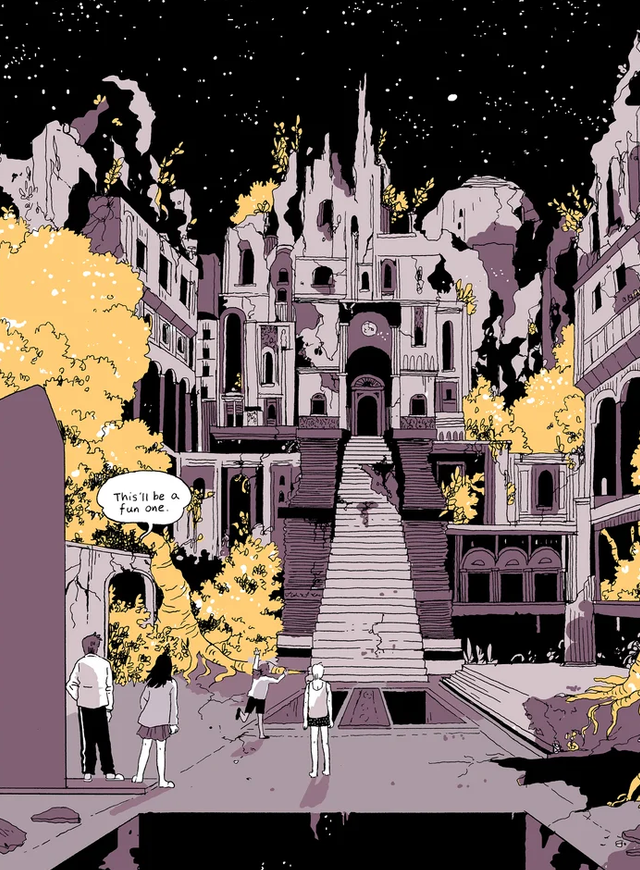
\includegraphics[width=\linewidth,height=.47\textheight,keepaspectratio]{assets/1795014338-sunbeam.png}\end{minipage}\par\medskip

\par\medskip{\color{rule}\hrule}\medskip
\begin{taskbox}
\tasktitle{Discuss}
\begin{enumerate}
\item Why did Mia sign up for the job? What did she expect and what did she get?
\item What do we learn about the society that used to exist where Mia and her crew do construction work?
\item What do we learn about Mia’s job?
\item Make a list of the names of the characters with a small description of who they are and how they are related to the other characters.
\end{enumerate}
\end{taskbox}

\section*{Analysis}
\tasktitle{Work with the text}
\begin{taskbox}
\tasktitle{Option A}
\begin{enumerate}
\item Write a manuscript for a presentation of the text. In your presentation of the text you must:

\begin{itemize}
\item sum up the main points of the text
\item relate the text to the theme
\item make an analysis of the theme of the text
\item speak for approx. 6 minutes
\end{itemize}

\end{enumerate}
\end{taskbox}
\begin{taskbox}
\tasktitle{Option B}
\begin{enumerate}
\item Chose a chapter to add captionboxes to.
\item Find at least 5 panels to write a caption box to. One of your panels must be a silent panel.
\item Take screenshots of the panels and add the boxes to the panels using e.g. canva.
\item Discuss with someone who also chose this option what and if your narrative voice adds anything significant to the story.
\end{enumerate}
\end{taskbox}

\clearpage\markboth{Space Westerns}{}
\phantomsection\addcontentsline{toc}{section}{9. Space Westerns}
{\color{blue}\small LESSON 09 \hfill 23 November 2026\par}
\vspace{4mm}
{\displayfont\color{navy}\fontsize{30}{34}\selectfont Space Westerns\par}\vspace{4mm}

\section*{Program}

\begin{itemize}
\item \emph{12.05} Westerns
\item \emph{12.15} The Lone Ranger
\item \emph{12.25} The Mandalorian
\item \emph{13.10} Break
\item \emph{13.25} Analysis
\item \emph{14.25} Break
\item \emph{14.35} Sum up
\end{itemize}

\section*{Westerns}
\begin{taskbox}
\tasktitle{Discuss}
\begin{enumerate}
\item What do you know about the film genre "westerns"?
\item Which movies have you watched / heard about / know the plot of?
\end{enumerate}
\end{taskbox}

\section*{The Lone Ranger}

\noindent\begin{minipage}[c]{.51\linewidth}
\begin{taskbox}
\tasktitle{Research}
\begin{enumerate}
\item Read about The Lone Ranger on wikipedia: How is he characterised?
\end{enumerate}
\end{taskbox}
\end{minipage}\hfill\begin{minipage}[c]{.44\linewidth}\centering
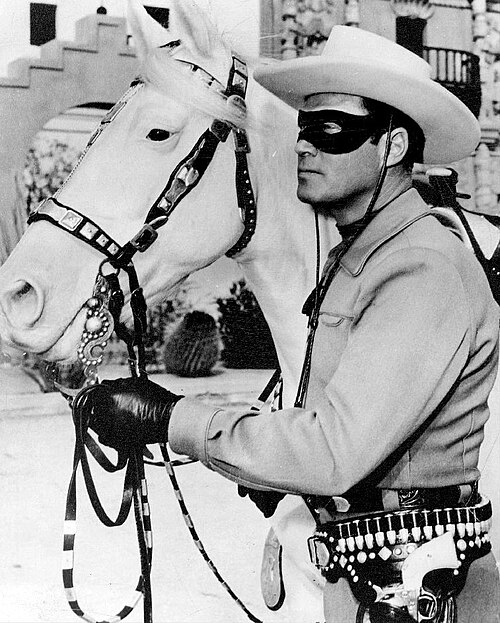
\includegraphics[width=\linewidth,height=.47\textheight,keepaspectratio]{assets/1795372840-loneranger.png}\end{minipage}\par\medskip

\section*{The Mandalorian}

\noindent\begin{minipage}[c]{.51\linewidth}
\begin{taskbox}
\tasktitle{Watch}
\begin{enumerate}
\item Watch the first episode of the tv-series The Mandalorian.
\end{enumerate}
\end{taskbox}
\end{minipage}\hfill\begin{minipage}[c]{.44\linewidth}\centering

\includegraphics[width=\linewidth,height=.47\textheight,keepaspectratio]{assets/1795372963-mando.png}\end{minipage}\par\medskip

\section*{Analysis}
\begin{taskbox}
\tasktitle{Analyse}
\begin{enumerate}
\item Use \hyperref[note-how-to-analyse]{this guide (p.~\pageref*{note-how-to-analyse})} to analyse the episode. Use only the parts of the guide you find relevant and interesting. Use what you know about western movies and The Lone Ranger in your analysis.
\end{enumerate}
\end{taskbox}

\clearpage\fancyhead[L]{\small\color{blue}Worksheets}

\clearpage\phantomsection\addcontentsline{toc}{chapter}{Worksheets}\markboth{Worksheets}{}
{\displayfont\color{navy}\fontsize{30}{34}\selectfont Worksheets\par}\vspace{6mm}
All worksheets referenced in the lessons are collected below. Click a title or page number to jump to the worksheet.\par
\tasktitle{Identity}
\begin{enumerate}
\item \hyperref[worksheet-1]{Who are you?} \hfill \hyperref[worksheet-1]{p.~\pageref*{worksheet-1}}
\item \hyperref[worksheet-2]{Identity in context} \hfill \hyperref[worksheet-2]{p.~\pageref*{worksheet-2}}
\item \hyperref[worksheet-3]{Molly's chapter - pacing questions} \hfill \hyperref[worksheet-3]{p.~\pageref*{worksheet-3}}
\item \hyperref[worksheet-4]{Molly's Room} \hfill \hyperref[worksheet-4]{p.~\pageref*{worksheet-4}}
\item \hyperref[worksheet-5]{Grammatik: Ordklasser} \hfill \hyperref[worksheet-5]{p.~\pageref*{worksheet-5}}
\item \hyperref[worksheet-6]{Calvin and Odin - pacing questions} \hfill \hyperref[worksheet-6]{p.~\pageref*{worksheet-6}}
\item \hyperref[worksheet-7]{Barbara's chapter} \hfill \hyperref[worksheet-7]{p.~\pageref*{worksheet-7}}
\item \hyperref[worksheet-8]{Walter's chapter} \hfill \hyperref[worksheet-8]{p.~\pageref*{worksheet-8}}
\item \hyperref[worksheet-9]{Clause Patterns — Worksheet} \hfill \hyperref[worksheet-9]{p.~\pageref*{worksheet-9}}
\item \hyperref[worksheet-10]{Edith - pacing questions} \hfill \hyperref[worksheet-10]{p.~\pageref*{worksheet-10}}
\end{enumerate}\tasktitle{Voice}\begin{enumerate}
\item \hyperref[worksheet-11]{Voice — Worksheet} \hfill \hyperref[worksheet-11]{p.~\pageref*{worksheet-11}}
\item \hyperref[worksheet-12]{dolls house — Worksheet} \hfill \hyperref[worksheet-12]{p.~\pageref*{worksheet-12}}
\item \hyperref[worksheet-13]{voice half crossword} \hfill \hyperref[worksheet-13]{p.~\pageref*{worksheet-13}}
\item \hyperref[worksheet-14]{The Kings Speech Rhetorical Situation} \hfill \hyperref[worksheet-14]{p.~\pageref*{worksheet-14}}
\end{enumerate}\tasktitle{The Future Is Written}\begin{enumerate}
\item \hyperref[worksheet-15]{Brave New World — Worksheet} \hfill \hyperref[worksheet-15]{p.~\pageref*{worksheet-15}}
\item \hyperref[worksheet-16]{Brave New World II — Worksheet} \hfill \hyperref[worksheet-16]{p.~\pageref*{worksheet-16}}
\item \hyperref[worksheet-17]{The Relive Box — Worksheet} \hfill \hyperref[worksheet-17]{p.~\pageref*{worksheet-17}}
\item \hyperref[worksheet-18]{US Space Policy — Worksheet} \hfill \hyperref[worksheet-18]{p.~\pageref*{worksheet-18}}
\item \hyperref[worksheet-19]{Settled In — Worksheet} \hfill \hyperref[worksheet-19]{p.~\pageref*{worksheet-19}}
\end{enumerate}

\clearpage\markboth{Who are you?}{}
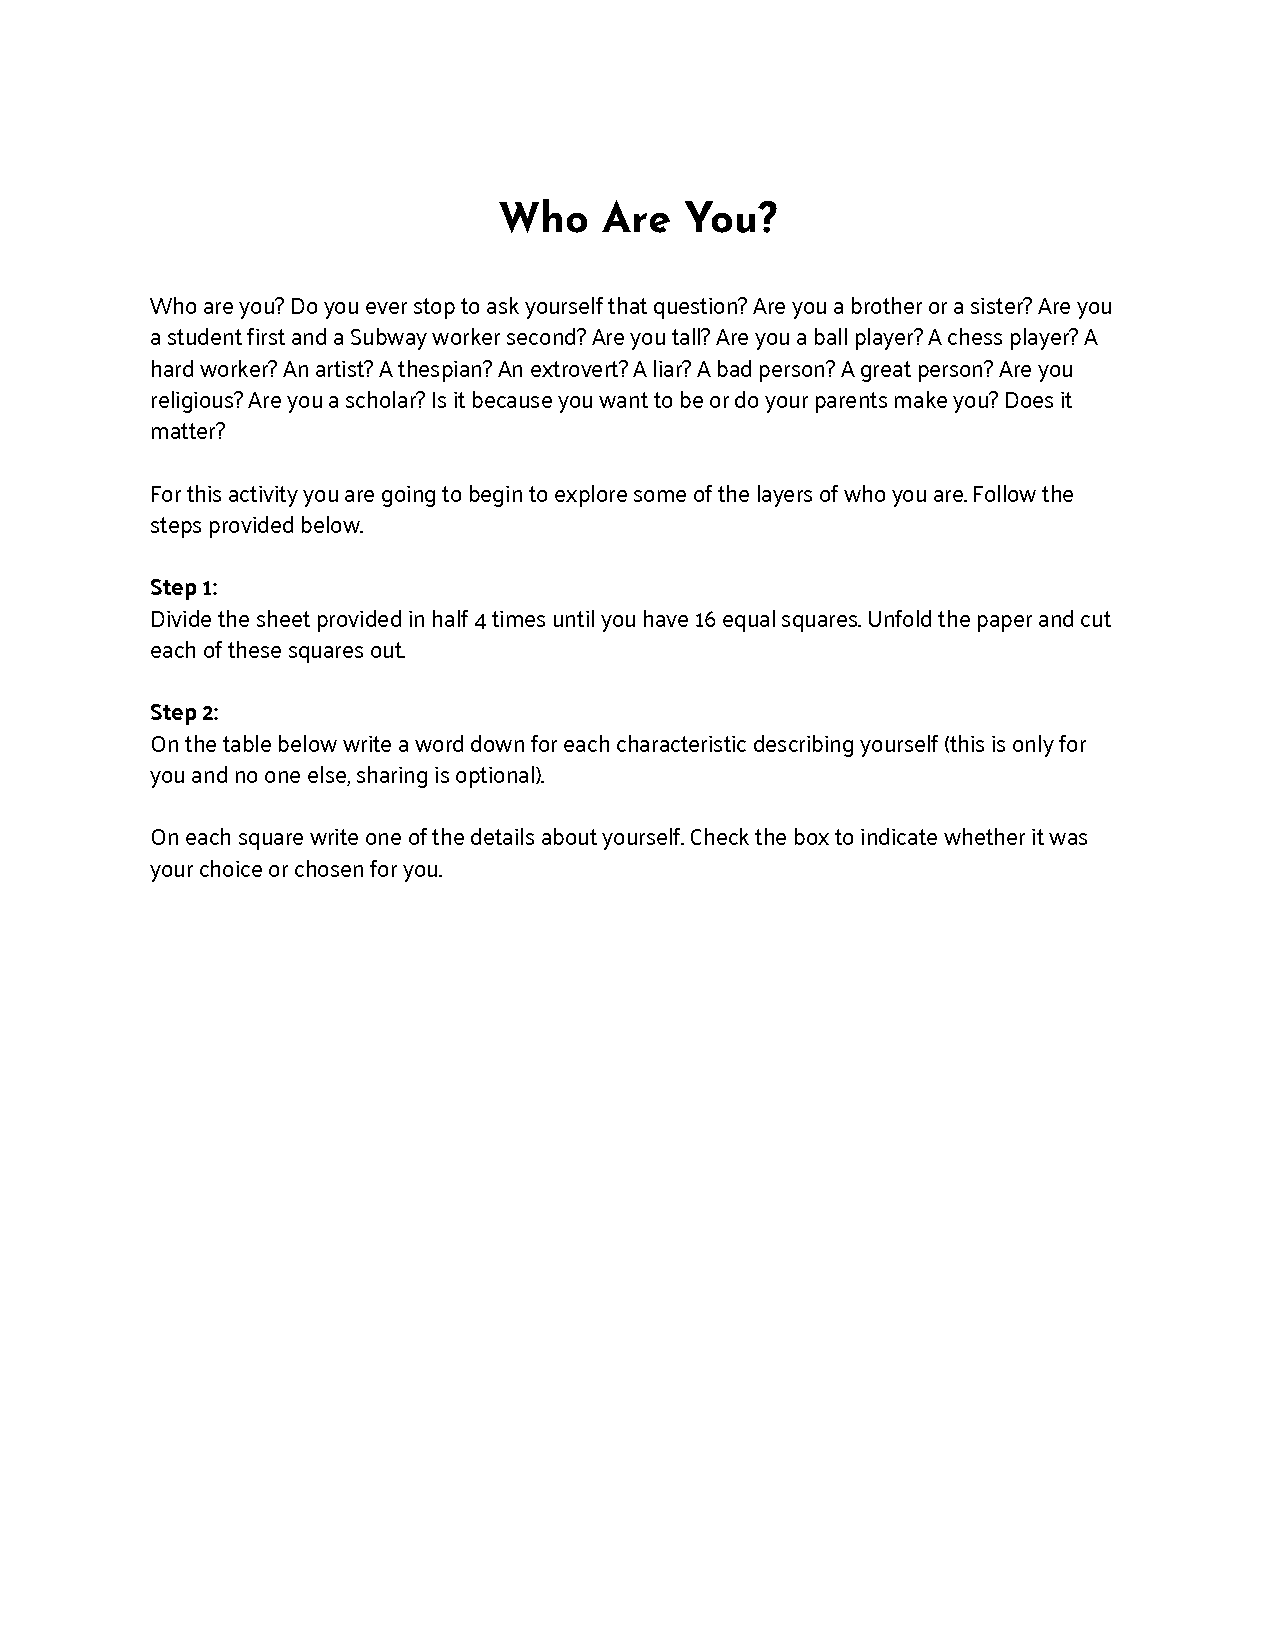
\includepdf[pages=-,scale=.9,pagecommand={\thispagestyle{fancy}},addtotoc={1,subsection,2,{Who are you?},worksheet-1}]{materials/iThrive_Who-Are-You-Activity.pdf}

\clearpage\markboth{Identity in context}{}
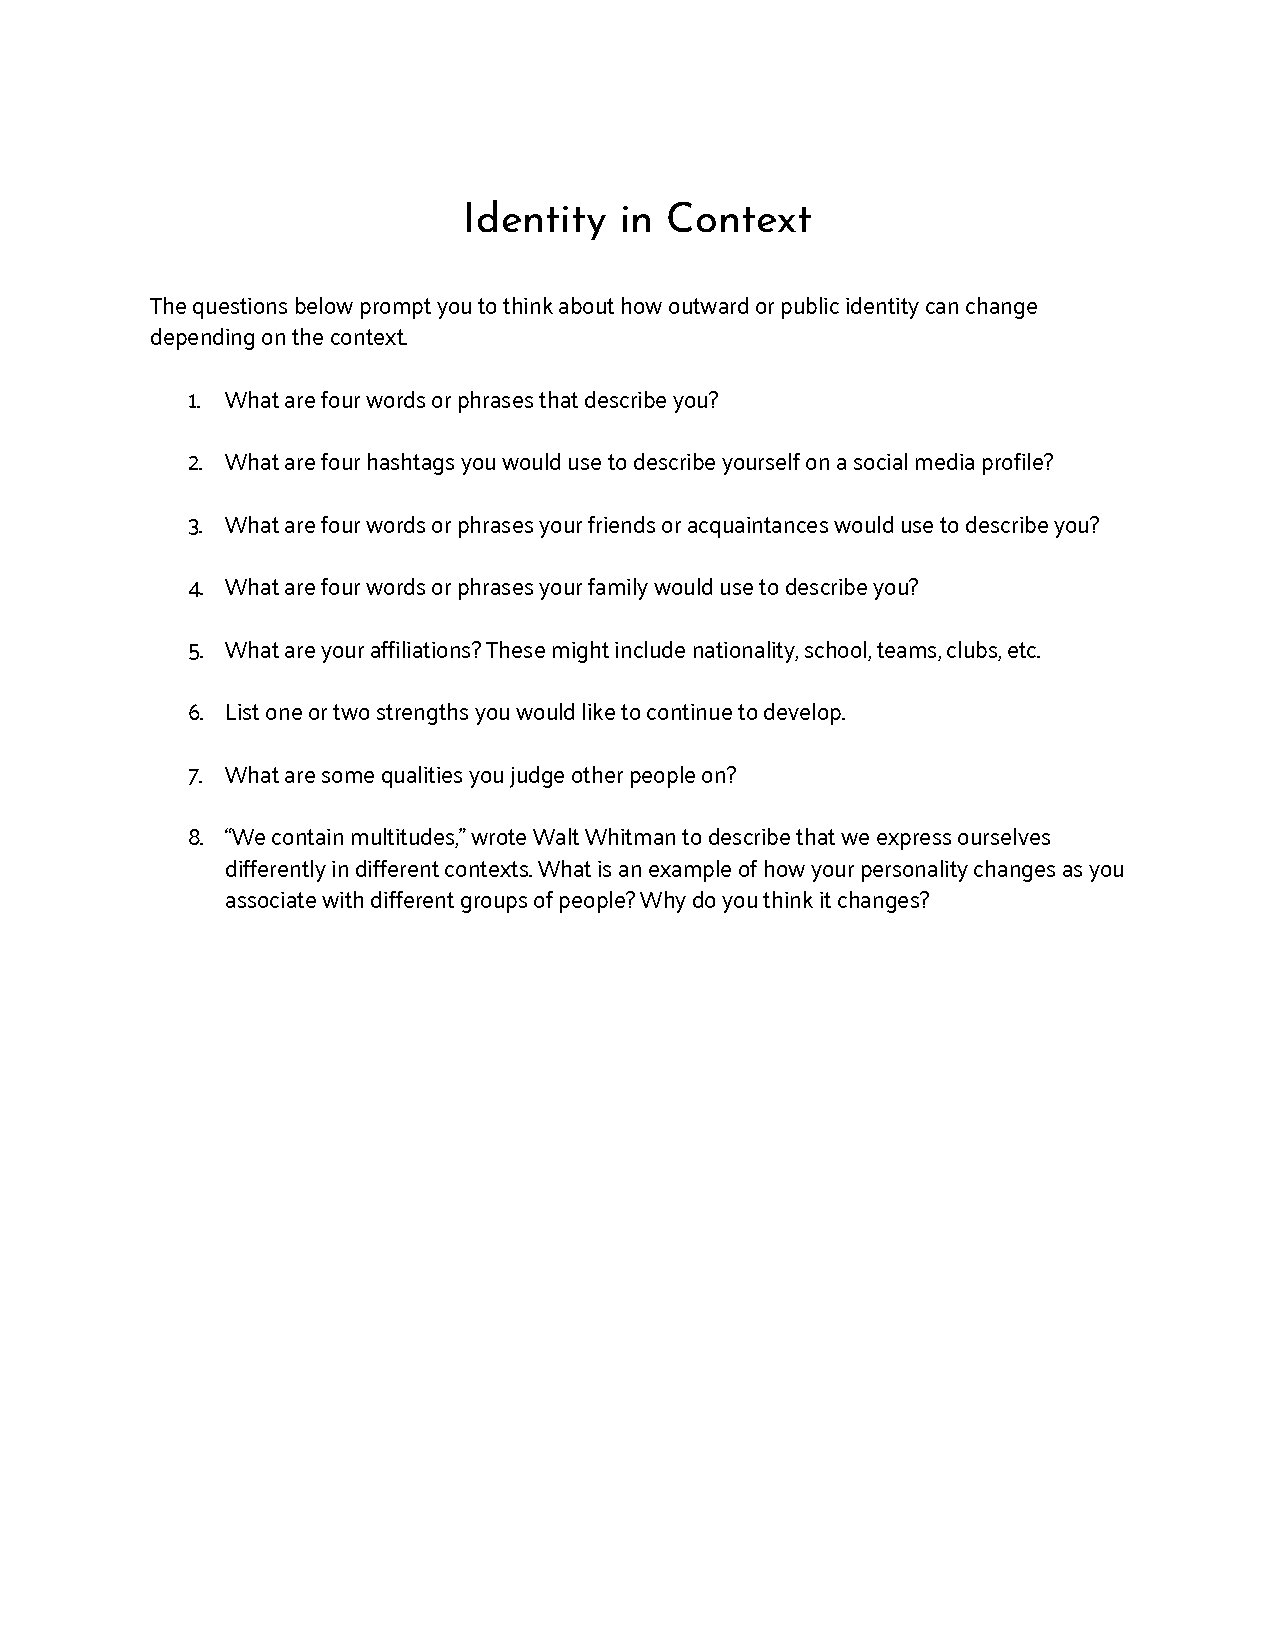
\includepdf[pages=-,scale=.9,pagecommand={\thispagestyle{fancy}},addtotoc={1,subsection,2,{Identity in context},worksheet-2}]{materials/iThrive__Identity_in_Context.pdf}

\clearpage\markboth{Molly's chapter - pacing questions}{}
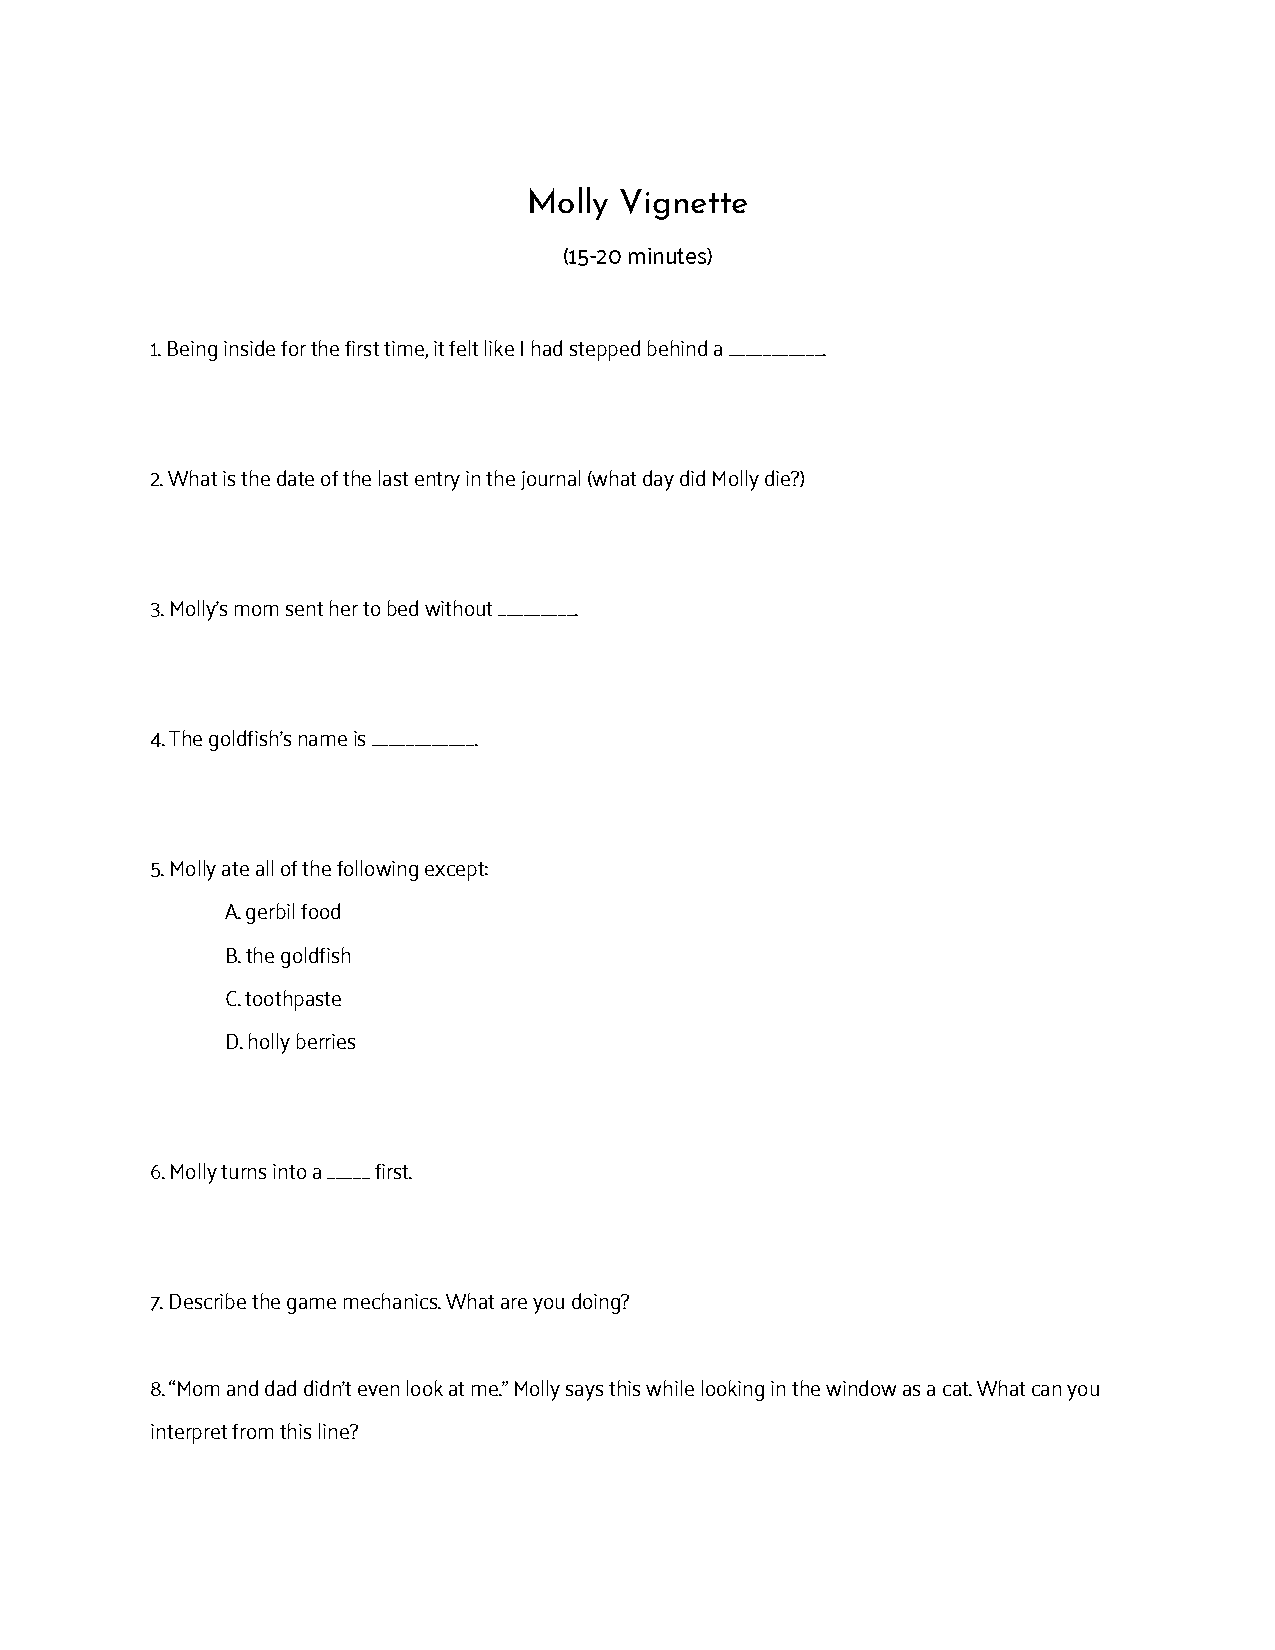
\includepdf[pages=-,scale=.9,pagecommand={\thispagestyle{fancy}},addtotoc={1,subsection,2,{Molly's chapter - pacing questions},worksheet-3}]{materials/2_Molly.pdf}

\clearpage\markboth{Molly's Room}{}
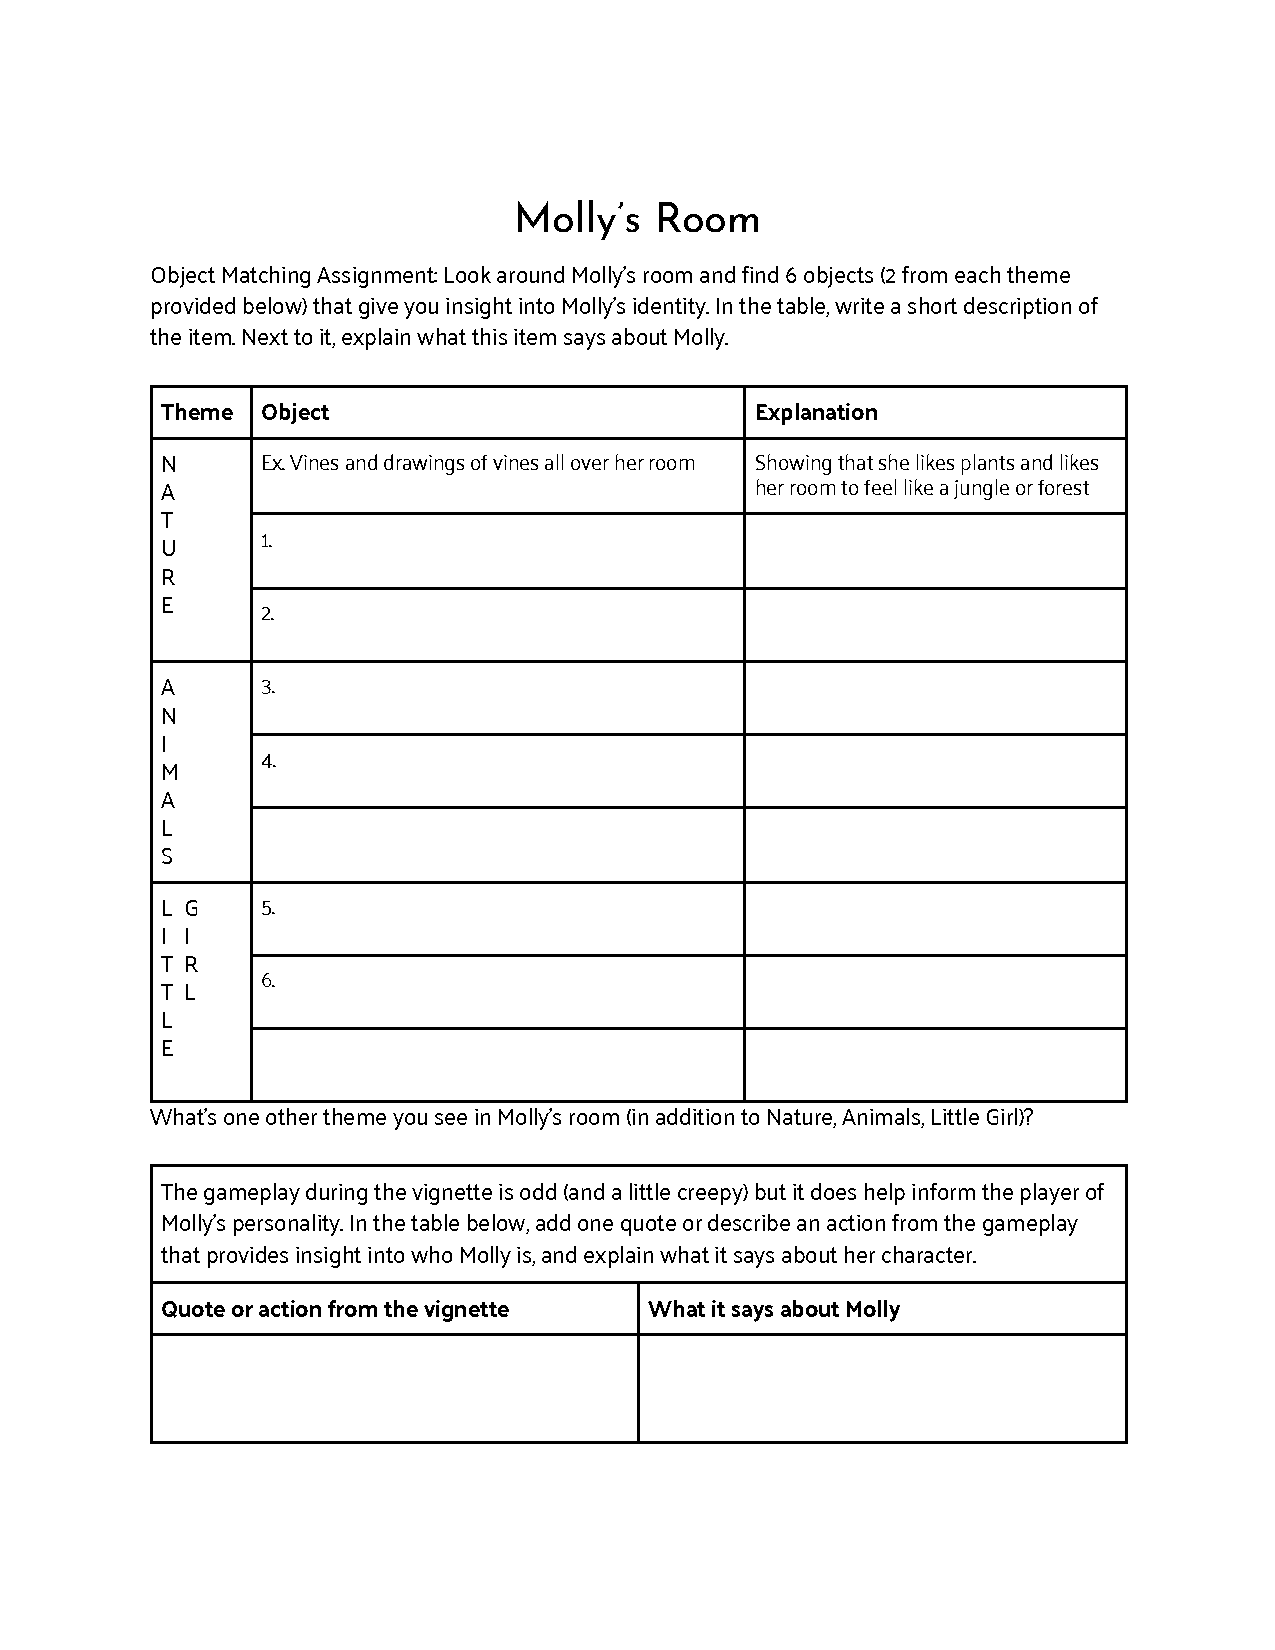
\includepdf[pages=-,scale=.9,pagecommand={\thispagestyle{fancy}},addtotoc={1,subsection,2,{Molly's Room},worksheet-4}]{materials/iThrive_Molly_Room_Assignment.pdf}

\clearpage\markboth{Grammatik: Ordklasser}{}
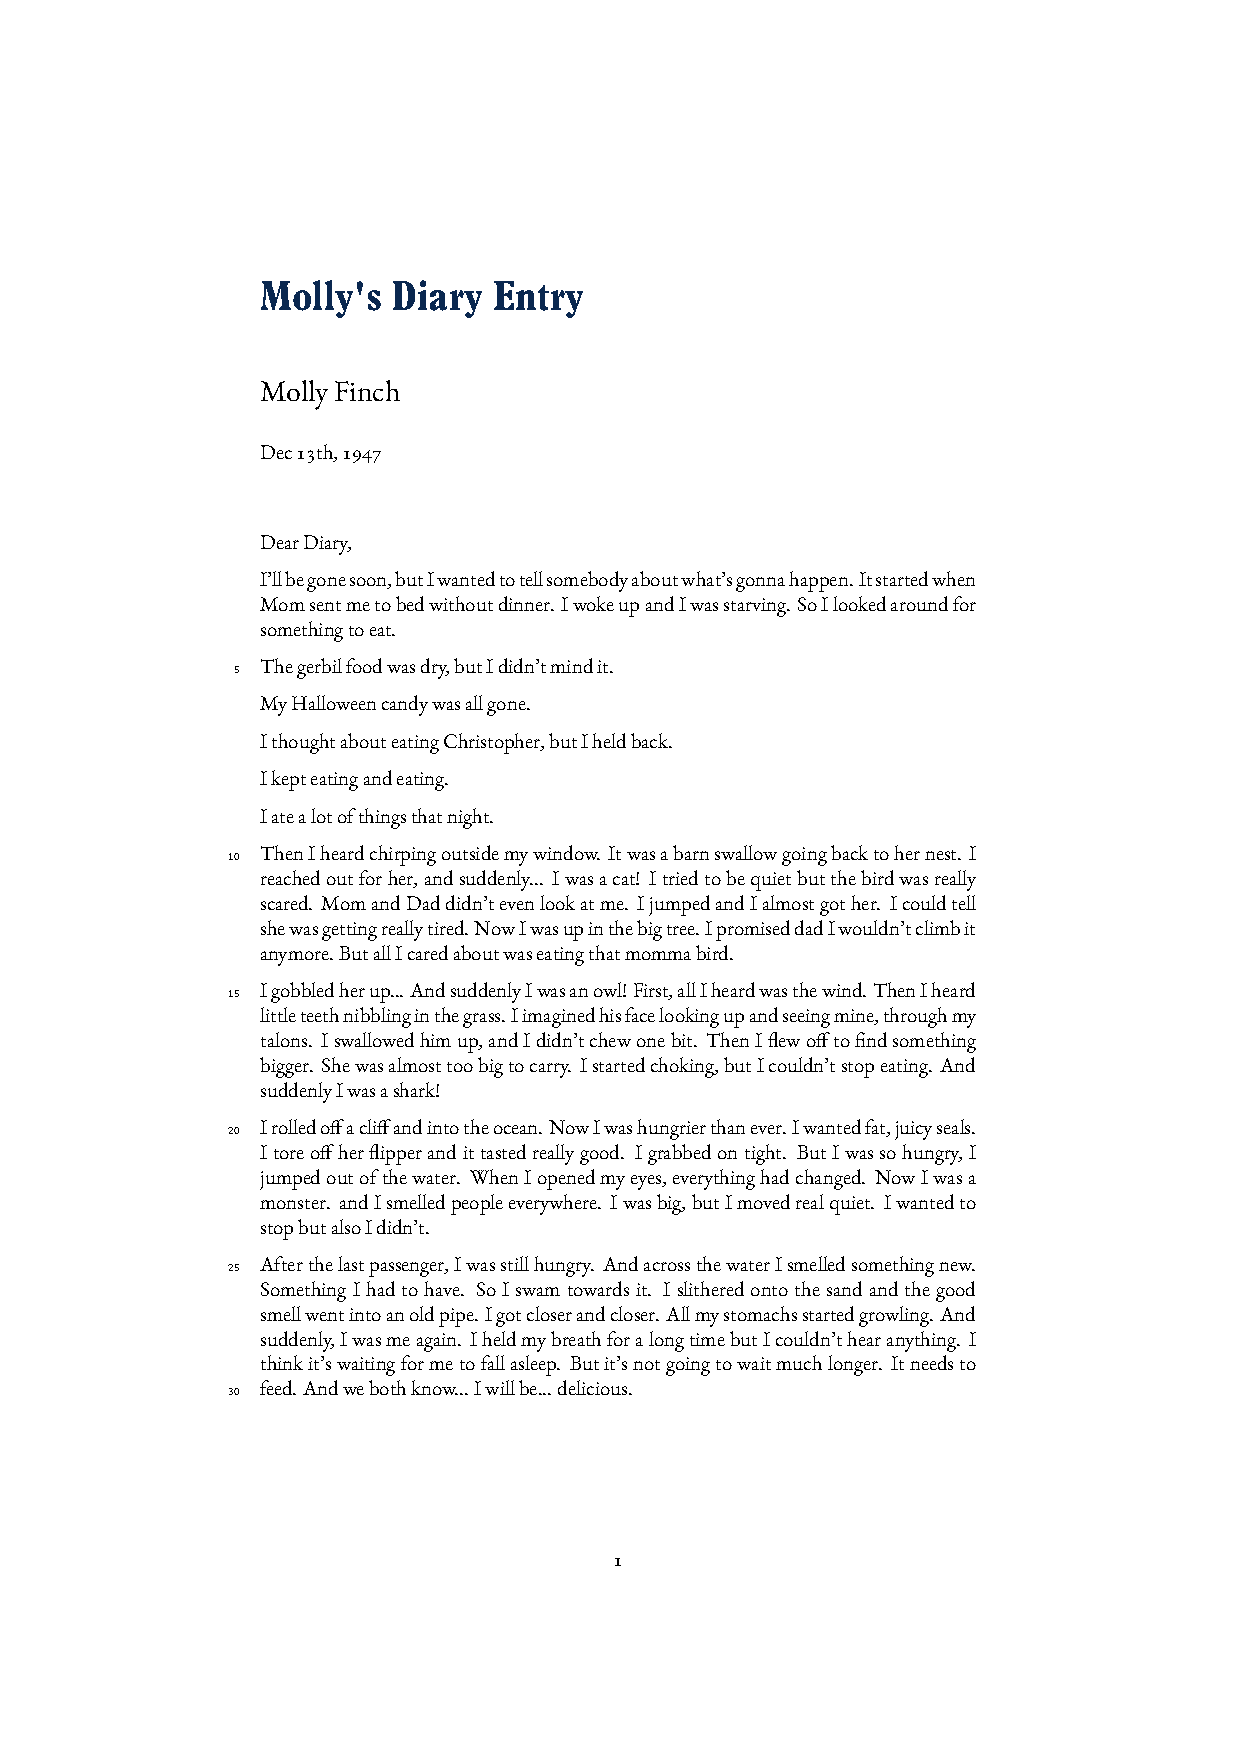
\includepdf[pages=-,scale=.9,pagecommand={\thispagestyle{fancy}},addtotoc={1,subsection,2,{Grammatik: Ordklasser},worksheet-5}]{materials/Mollys_Diary_Entry.pdf}

\clearpage\markboth{Calvin and Odin - pacing questions}{}
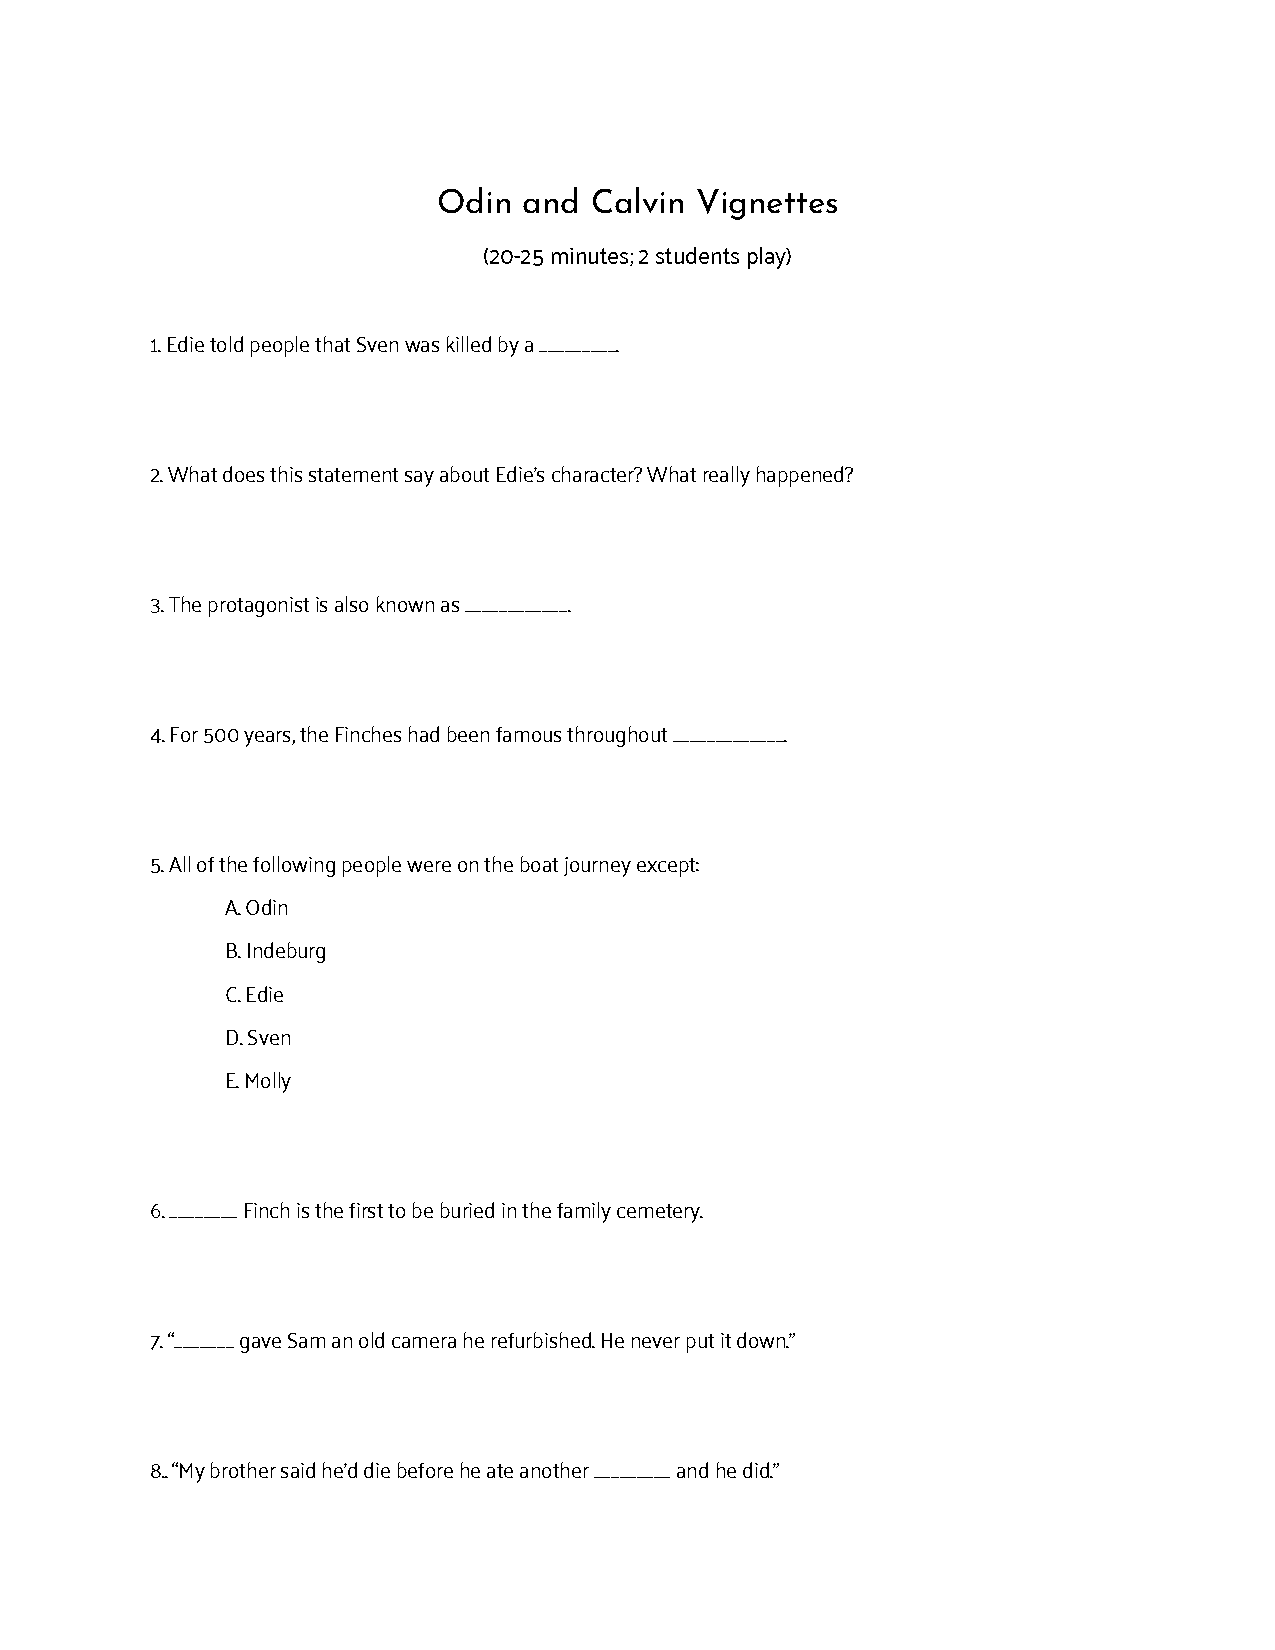
\includepdf[pages=-,scale=.9,pagecommand={\thispagestyle{fancy}},addtotoc={1,subsection,2,{Calvin and Odin - pacing questions},worksheet-6}]{materials/4_Odin_and_Calvin.pdf}

\clearpage\markboth{Barbara's chapter}{}
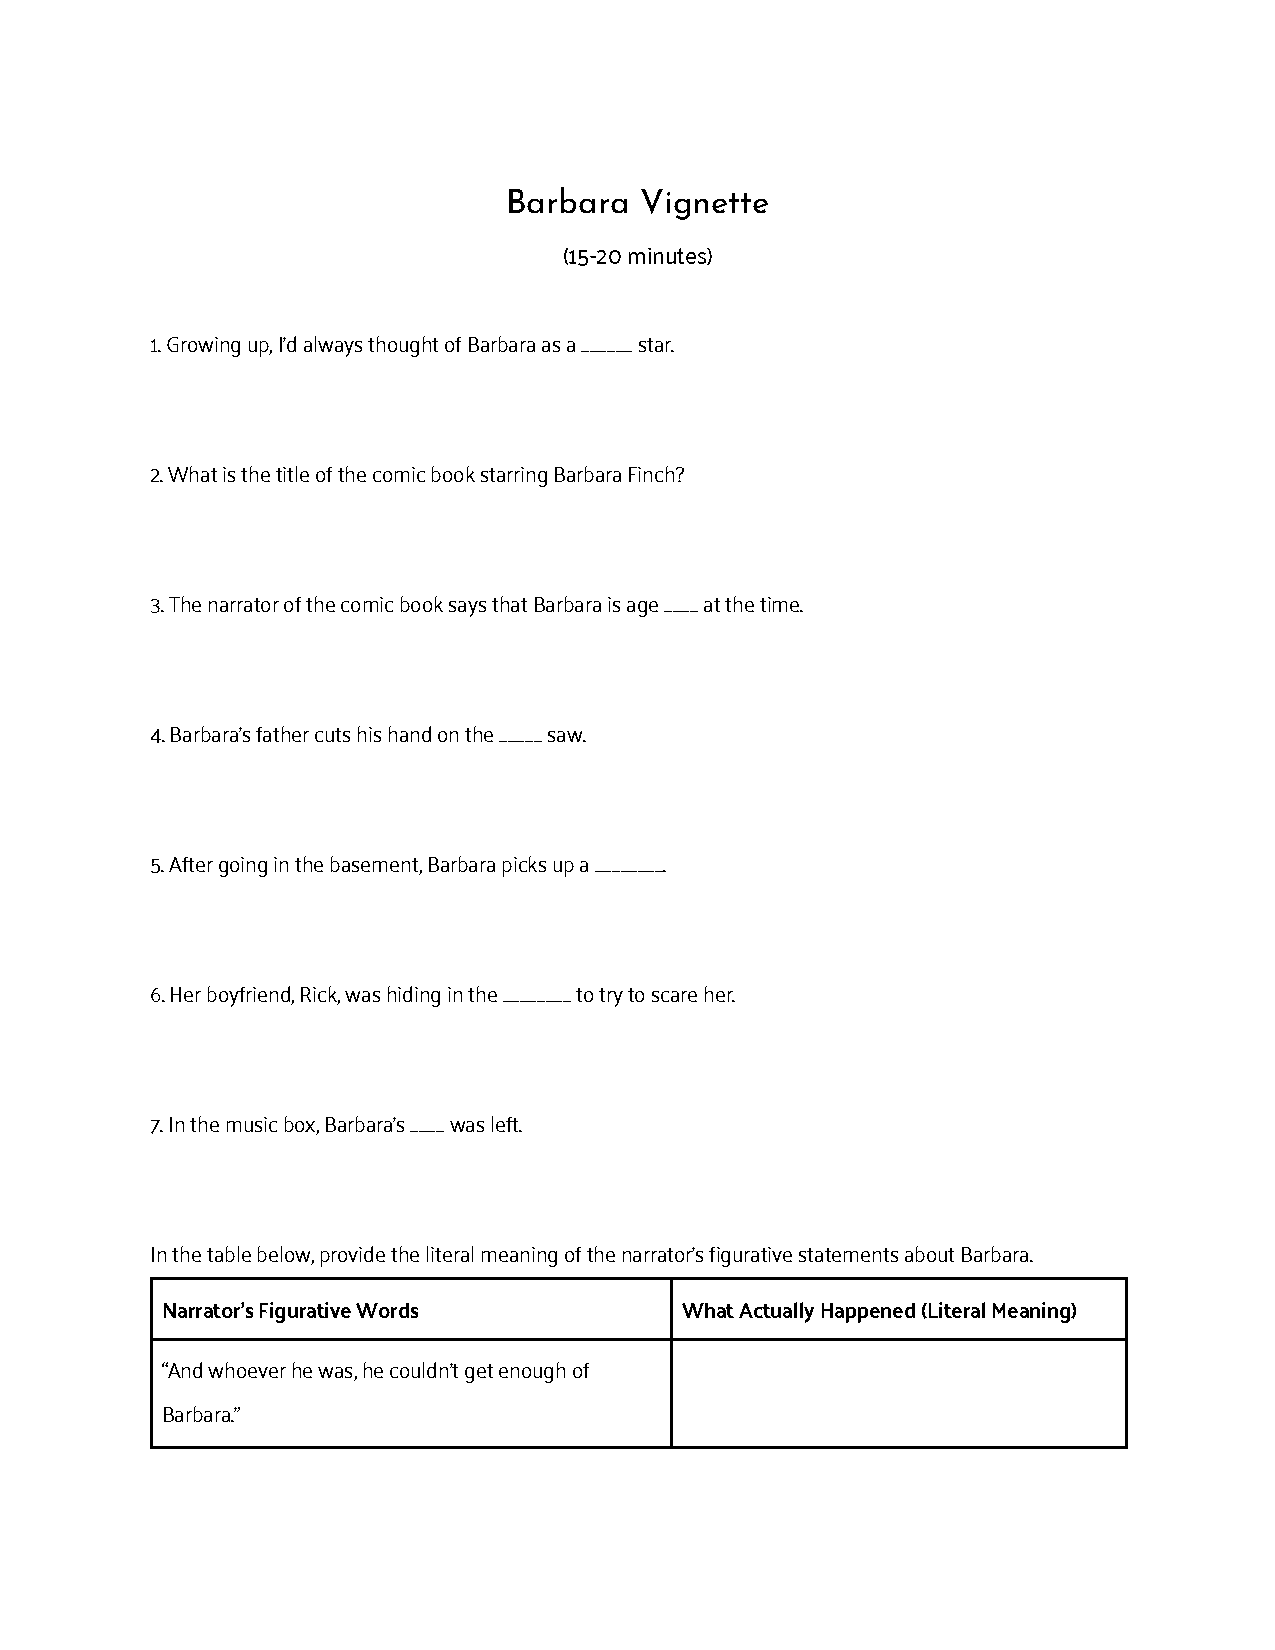
\includepdf[pages=-,scale=.9,pagecommand={\thispagestyle{fancy}},addtotoc={1,subsection,2,{Barbara's chapter},worksheet-7}]{materials/3_Barbara.pdf}

\clearpage\markboth{Walter's chapter}{}
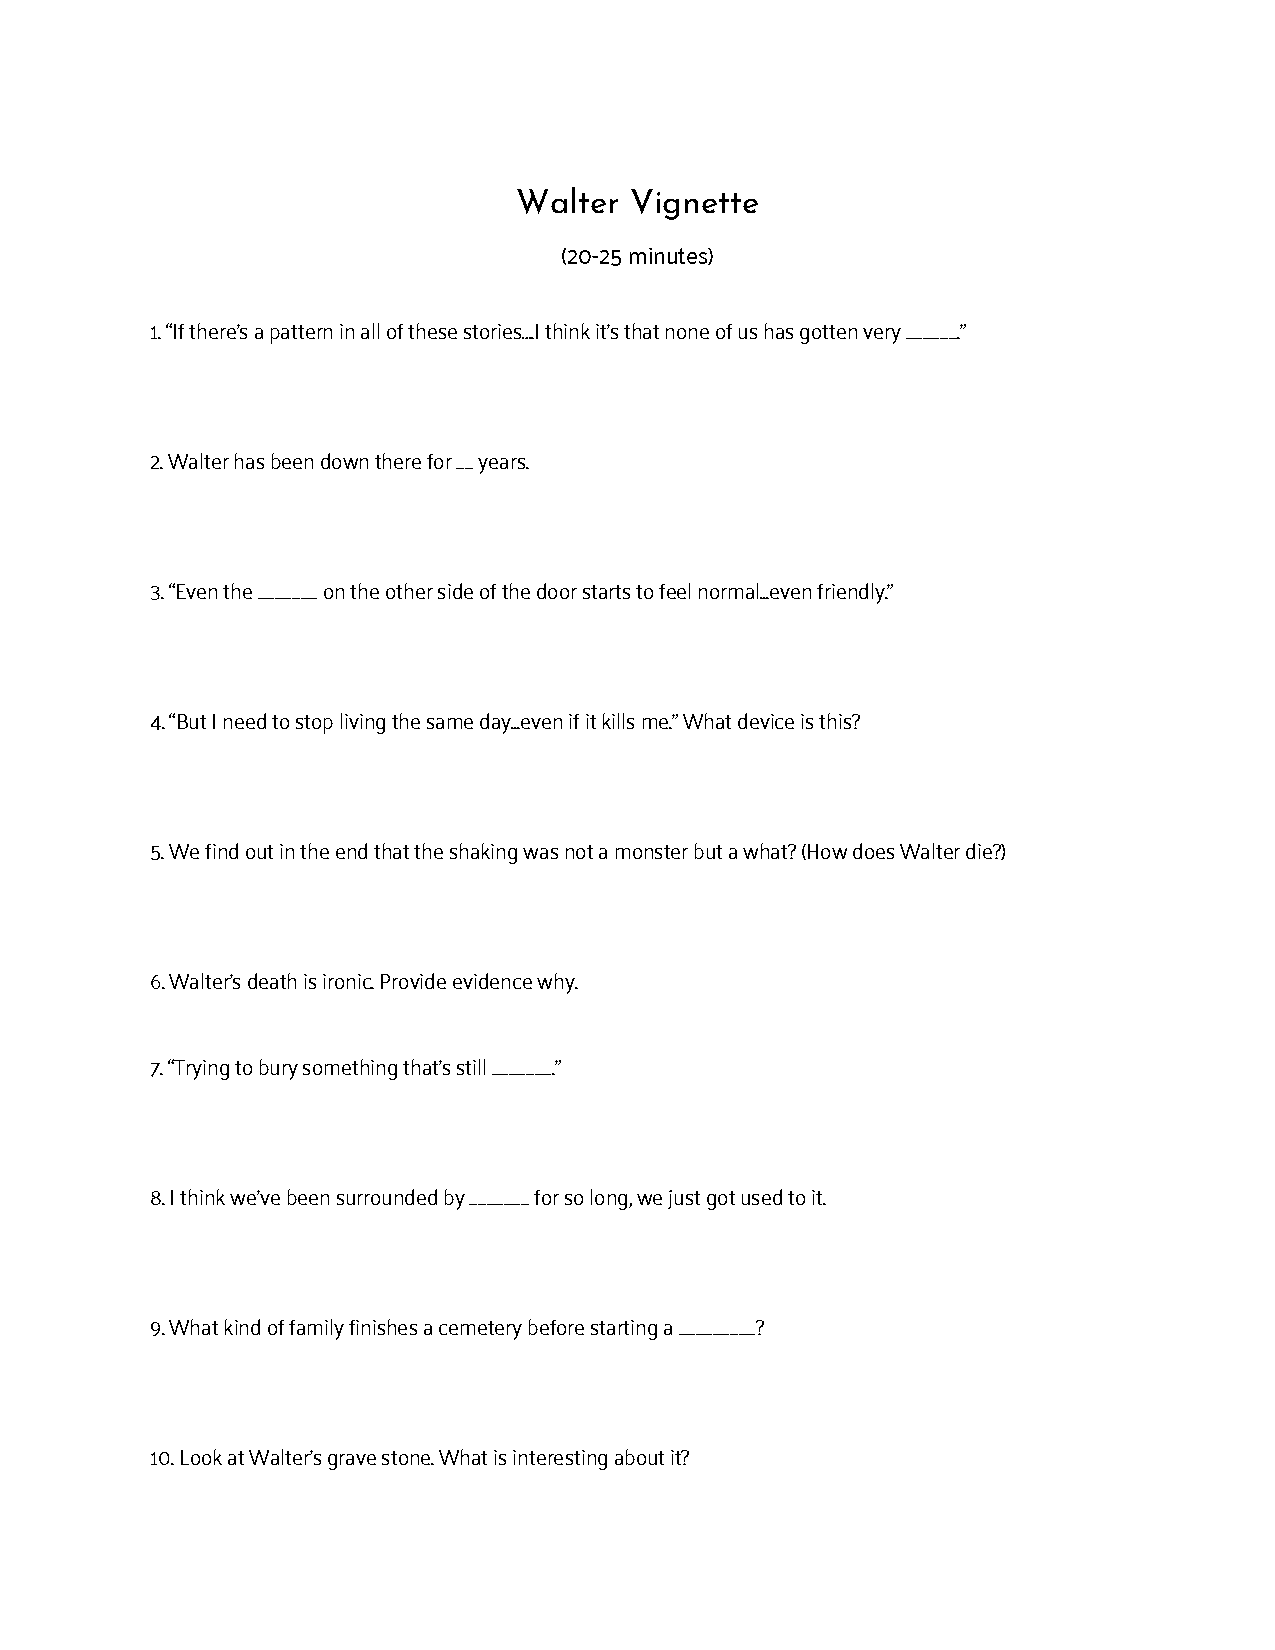
\includepdf[pages=-,scale=.9,pagecommand={\thispagestyle{fancy}},addtotoc={1,subsection,2,{Walter's chapter},worksheet-8}]{materials/5_Walter.pdf}

\clearpage\markboth{Clause Patterns — Worksheet}{}
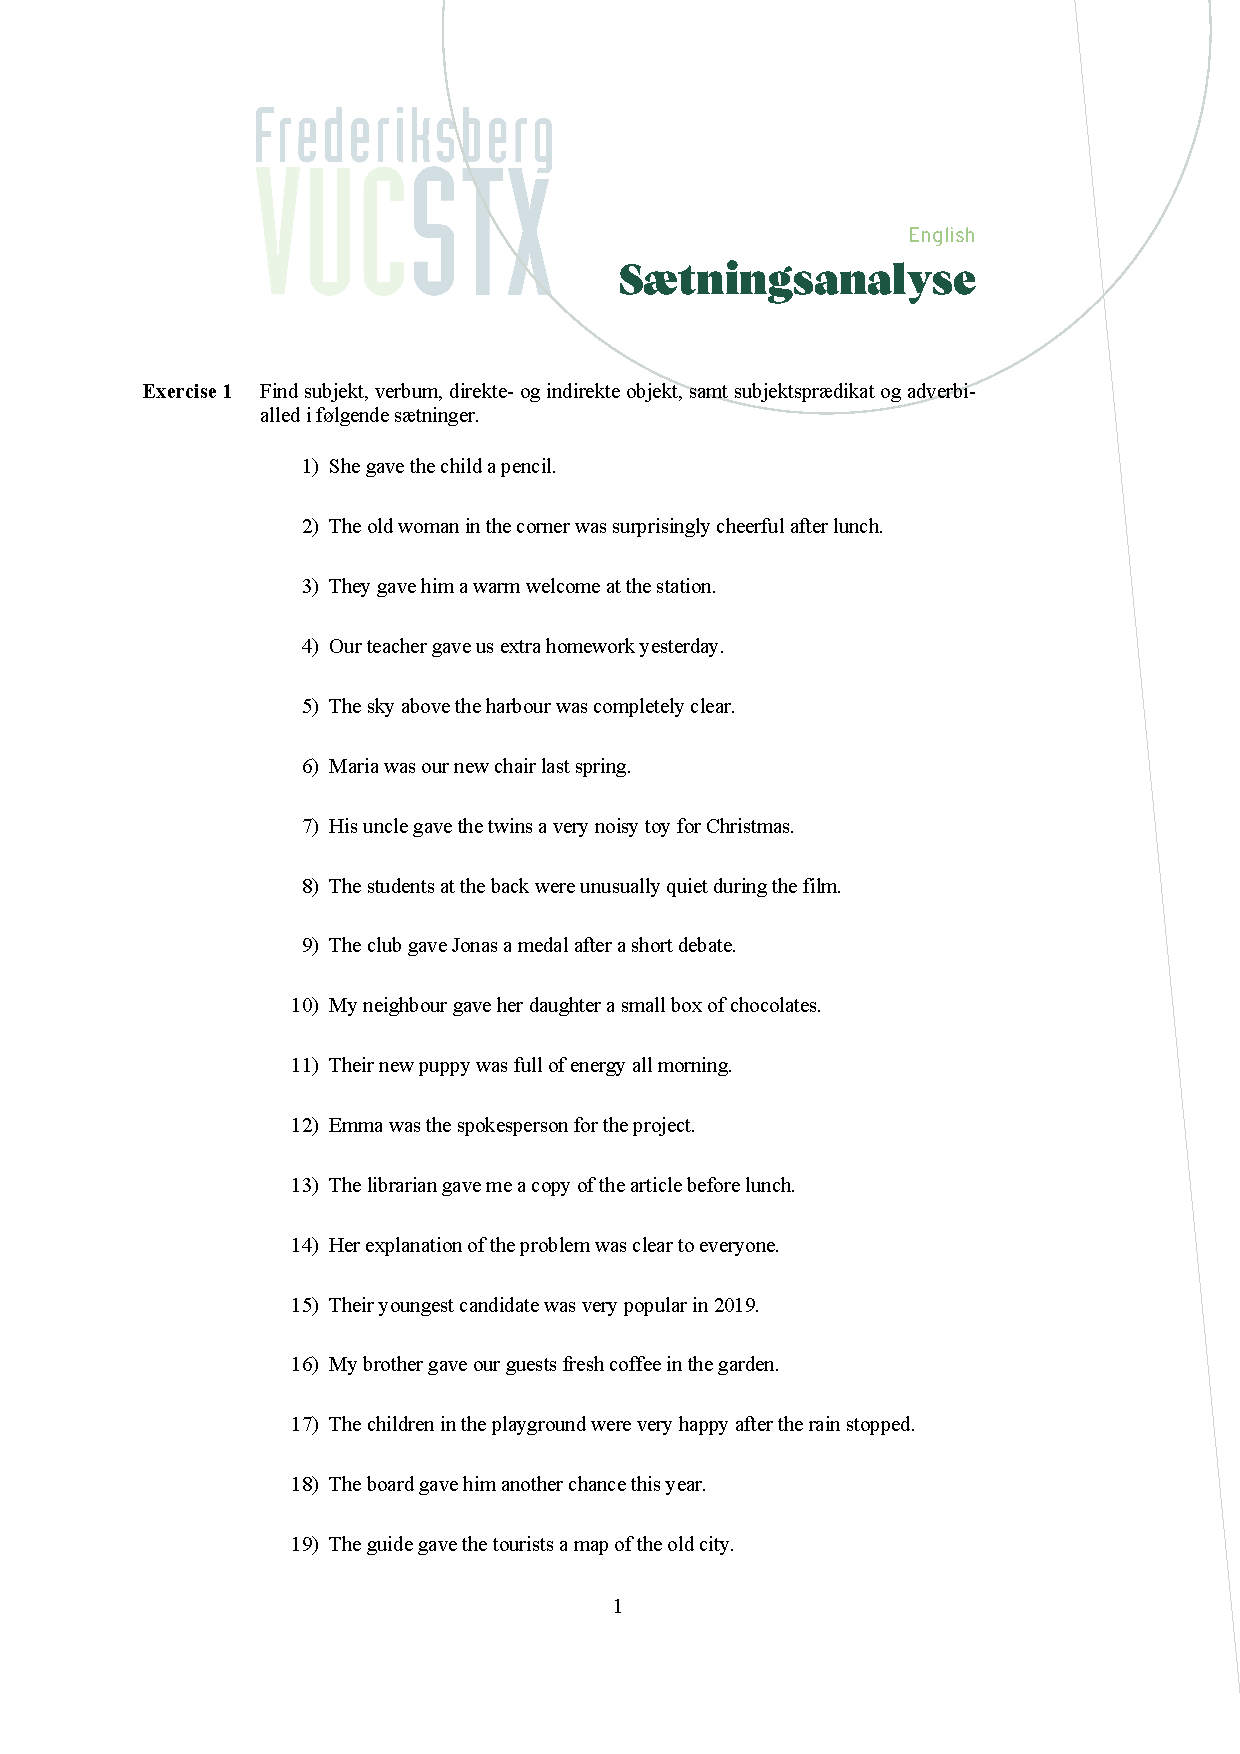
\includepdf[pages=-,scale=.9,pagecommand={\thispagestyle{fancy}},addtotoc={1,subsection,2,{Clause Patterns — Worksheet},worksheet-9}]{materials/Clause_Patterns_Worksheet.pdf}

\clearpage\markboth{Edith - pacing questions}{}
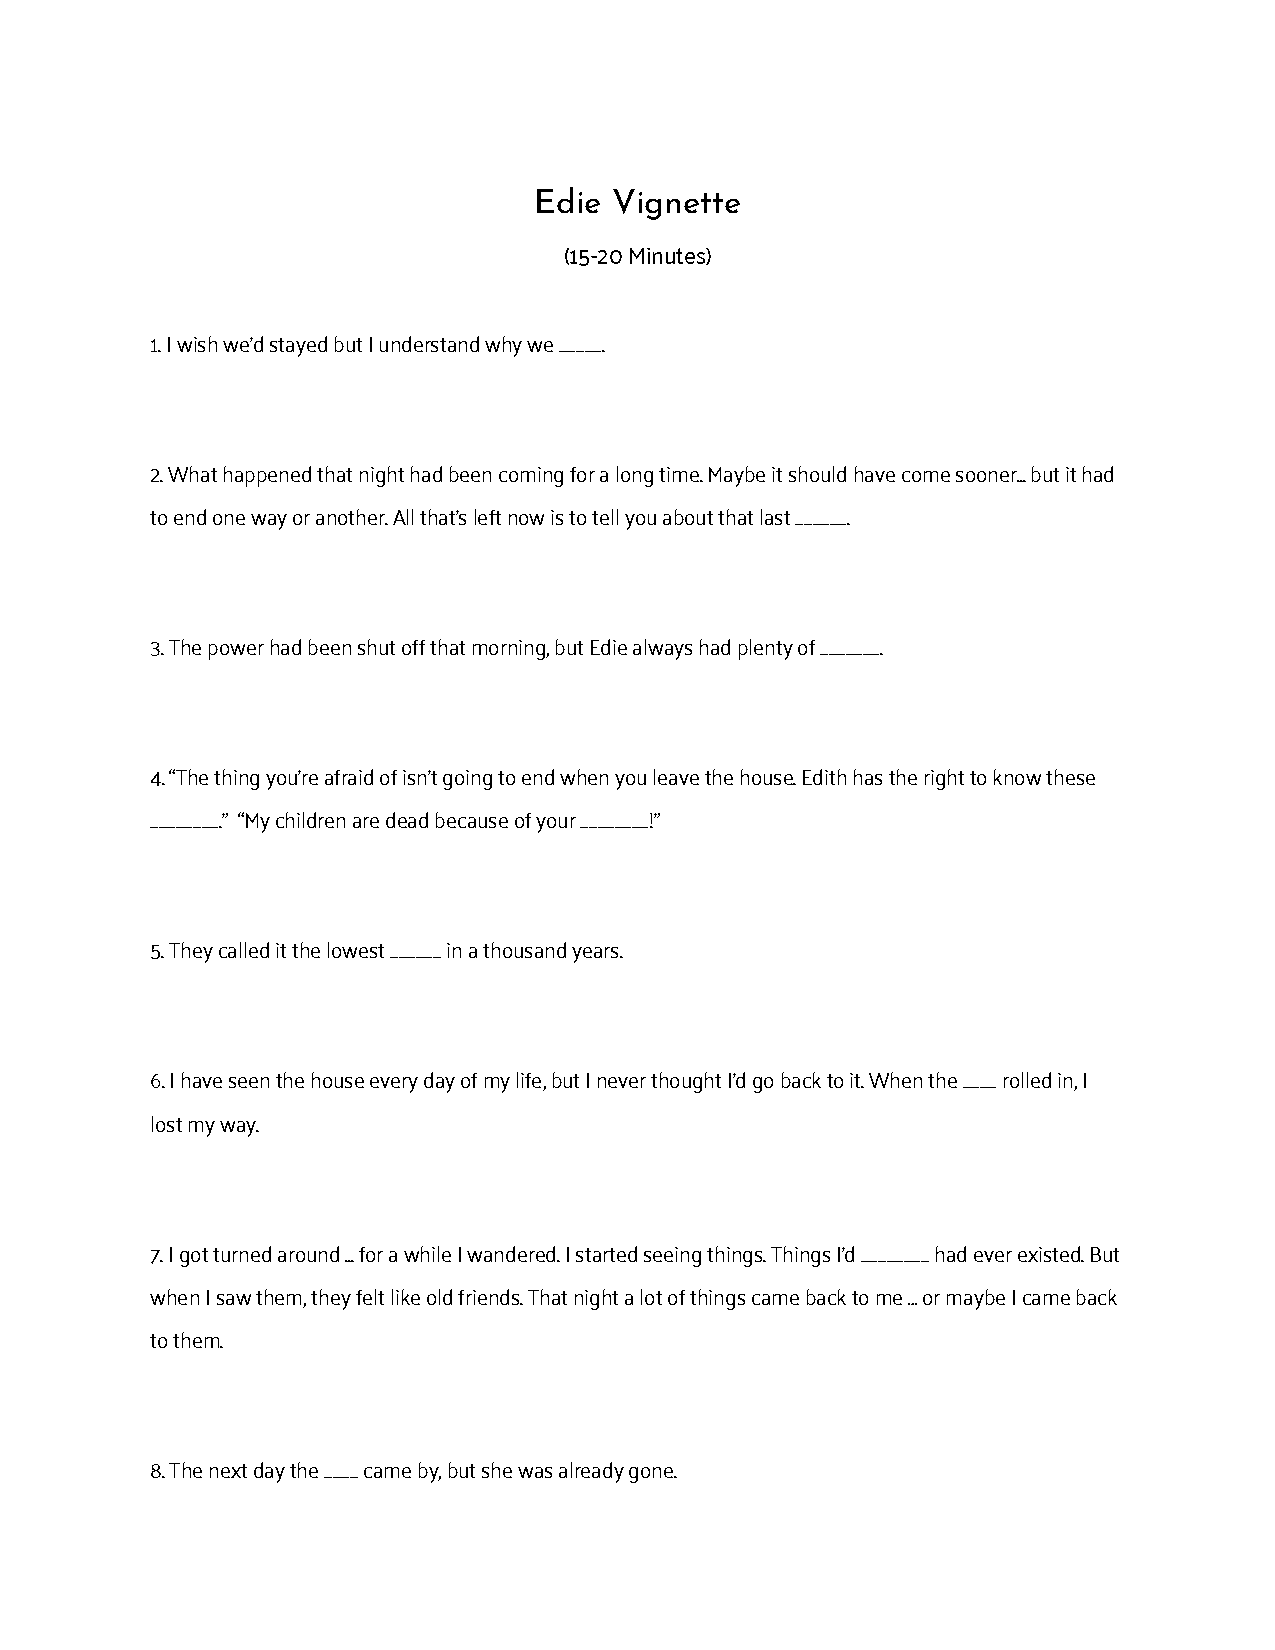
\includepdf[pages=-,scale=.9,pagecommand={\thispagestyle{fancy}},addtotoc={1,subsection,2,{Edith - pacing questions},worksheet-10}]{materials/9_Edie.pdf}

\clearpage\markboth{Voice — Worksheet}{}
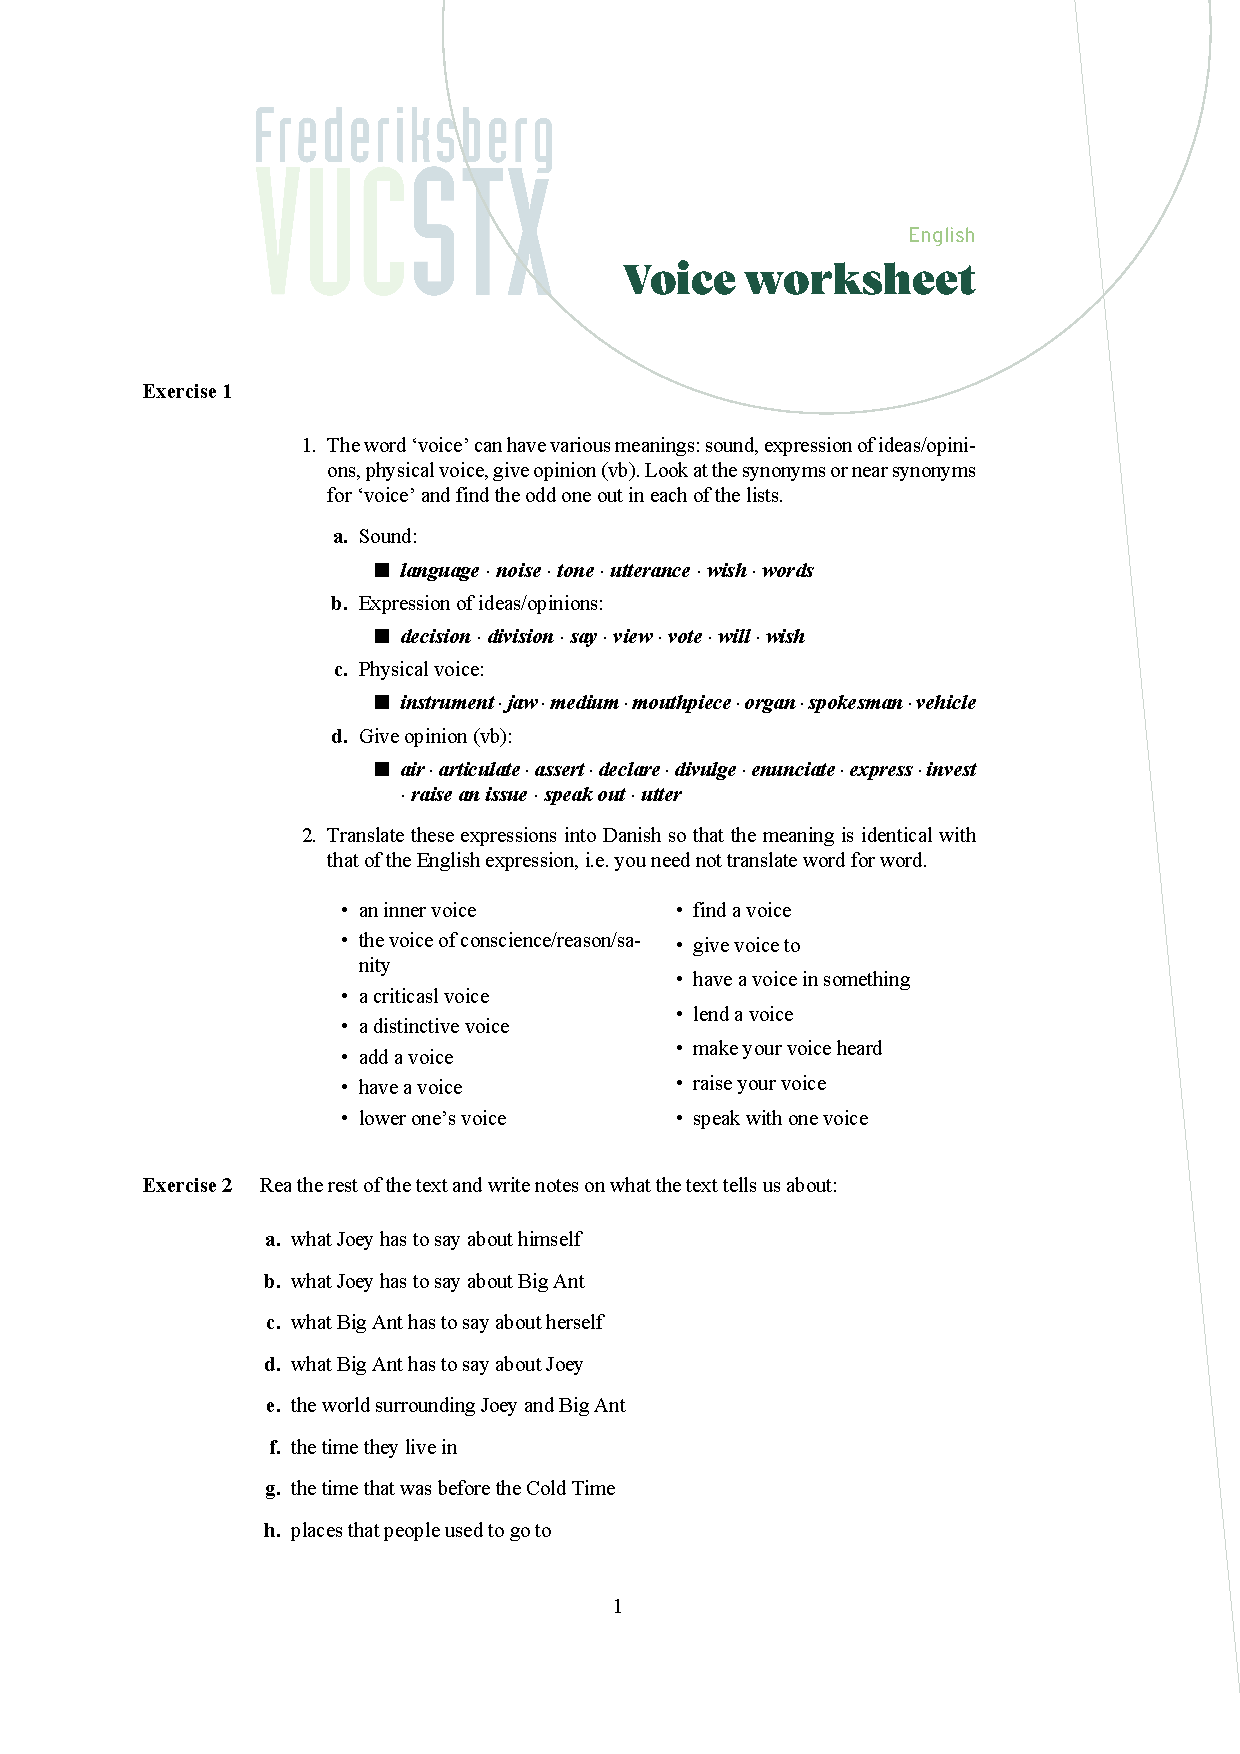
\includepdf[pages=-,scale=.9,pagecommand={\thispagestyle{fancy}},addtotoc={1,subsection,2,{Voice — Worksheet},worksheet-11}]{materials/Voice_Worksheet.pdf}

\clearpage\markboth{dolls house — Worksheet}{}
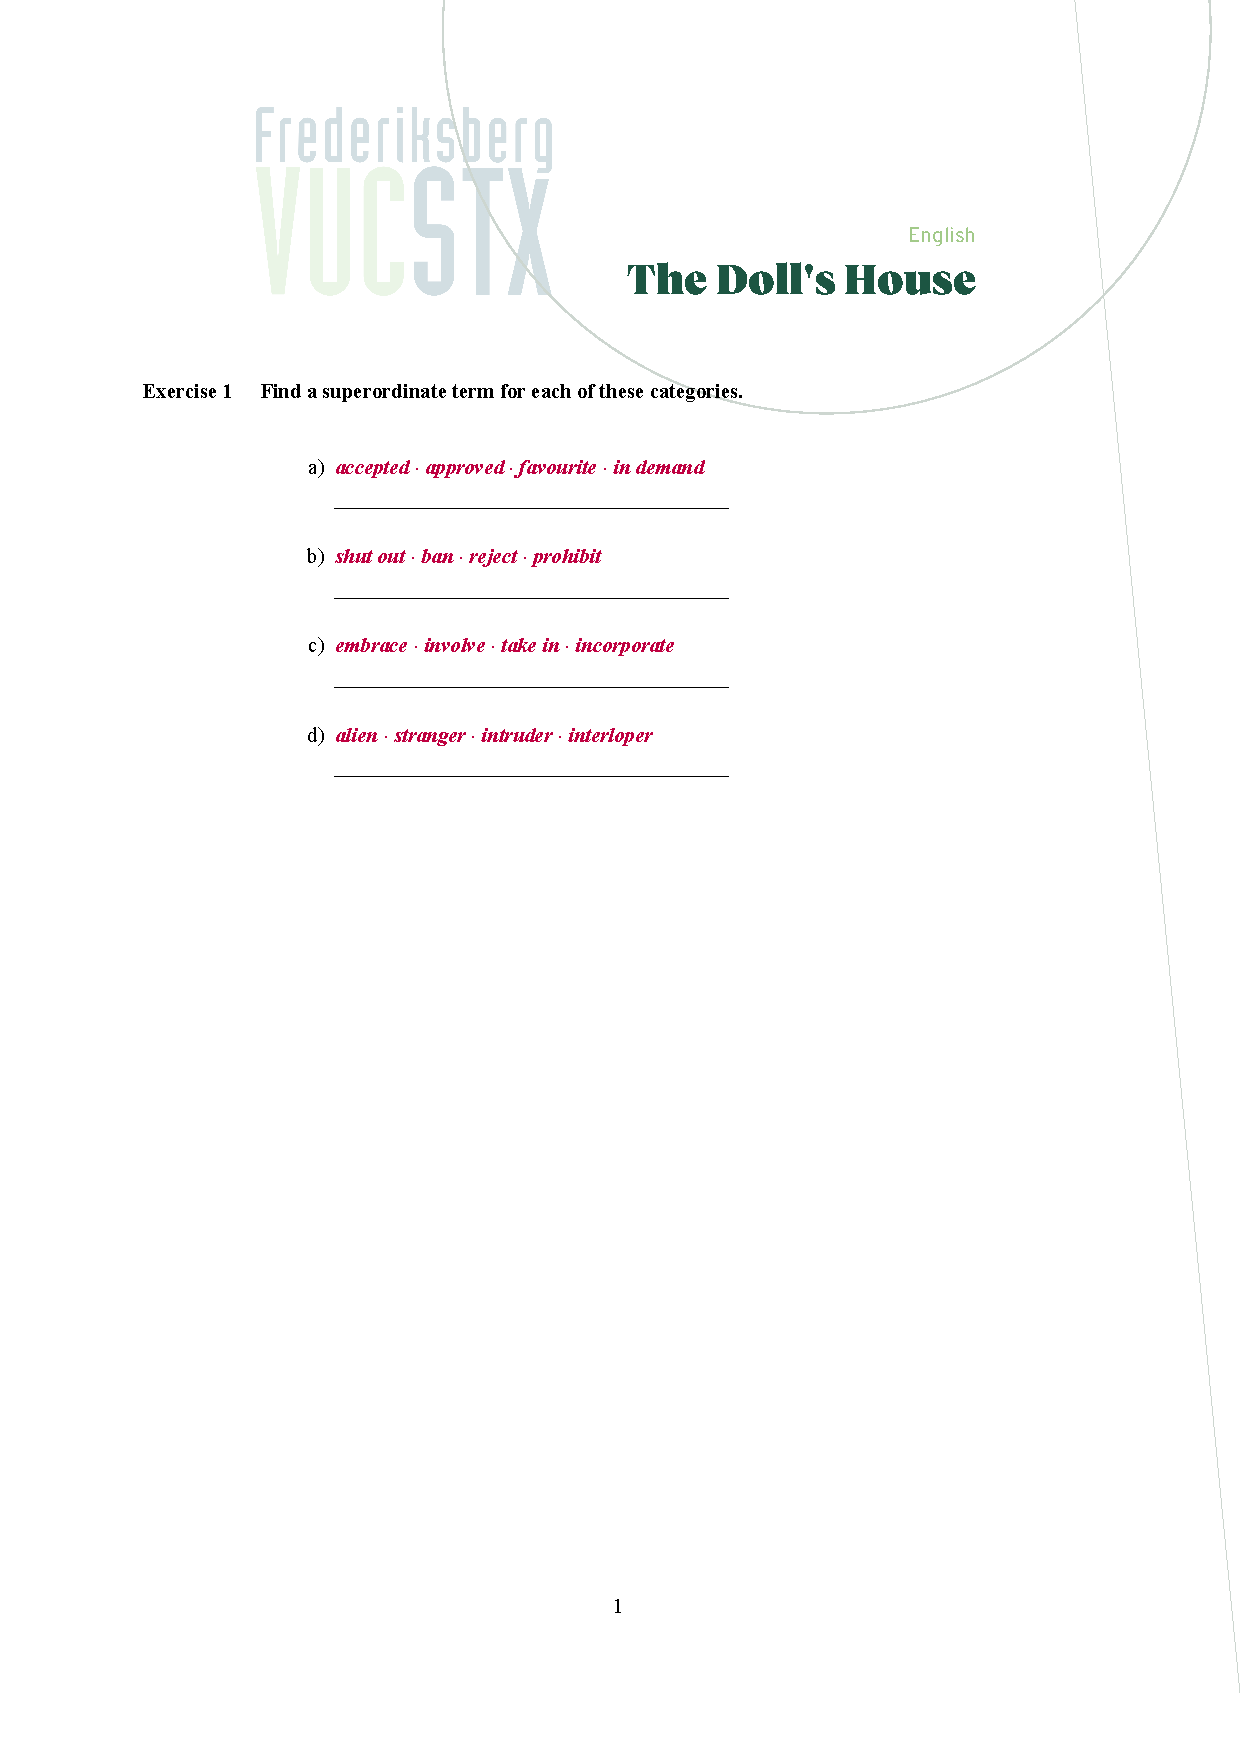
\includepdf[pages=-,scale=.9,pagecommand={\thispagestyle{fancy}},addtotoc={1,subsection,2,{dolls house — Worksheet},worksheet-12}]{materials/dolls_house_worksheet.pdf}

\clearpage\markboth{voice half crossword}{}
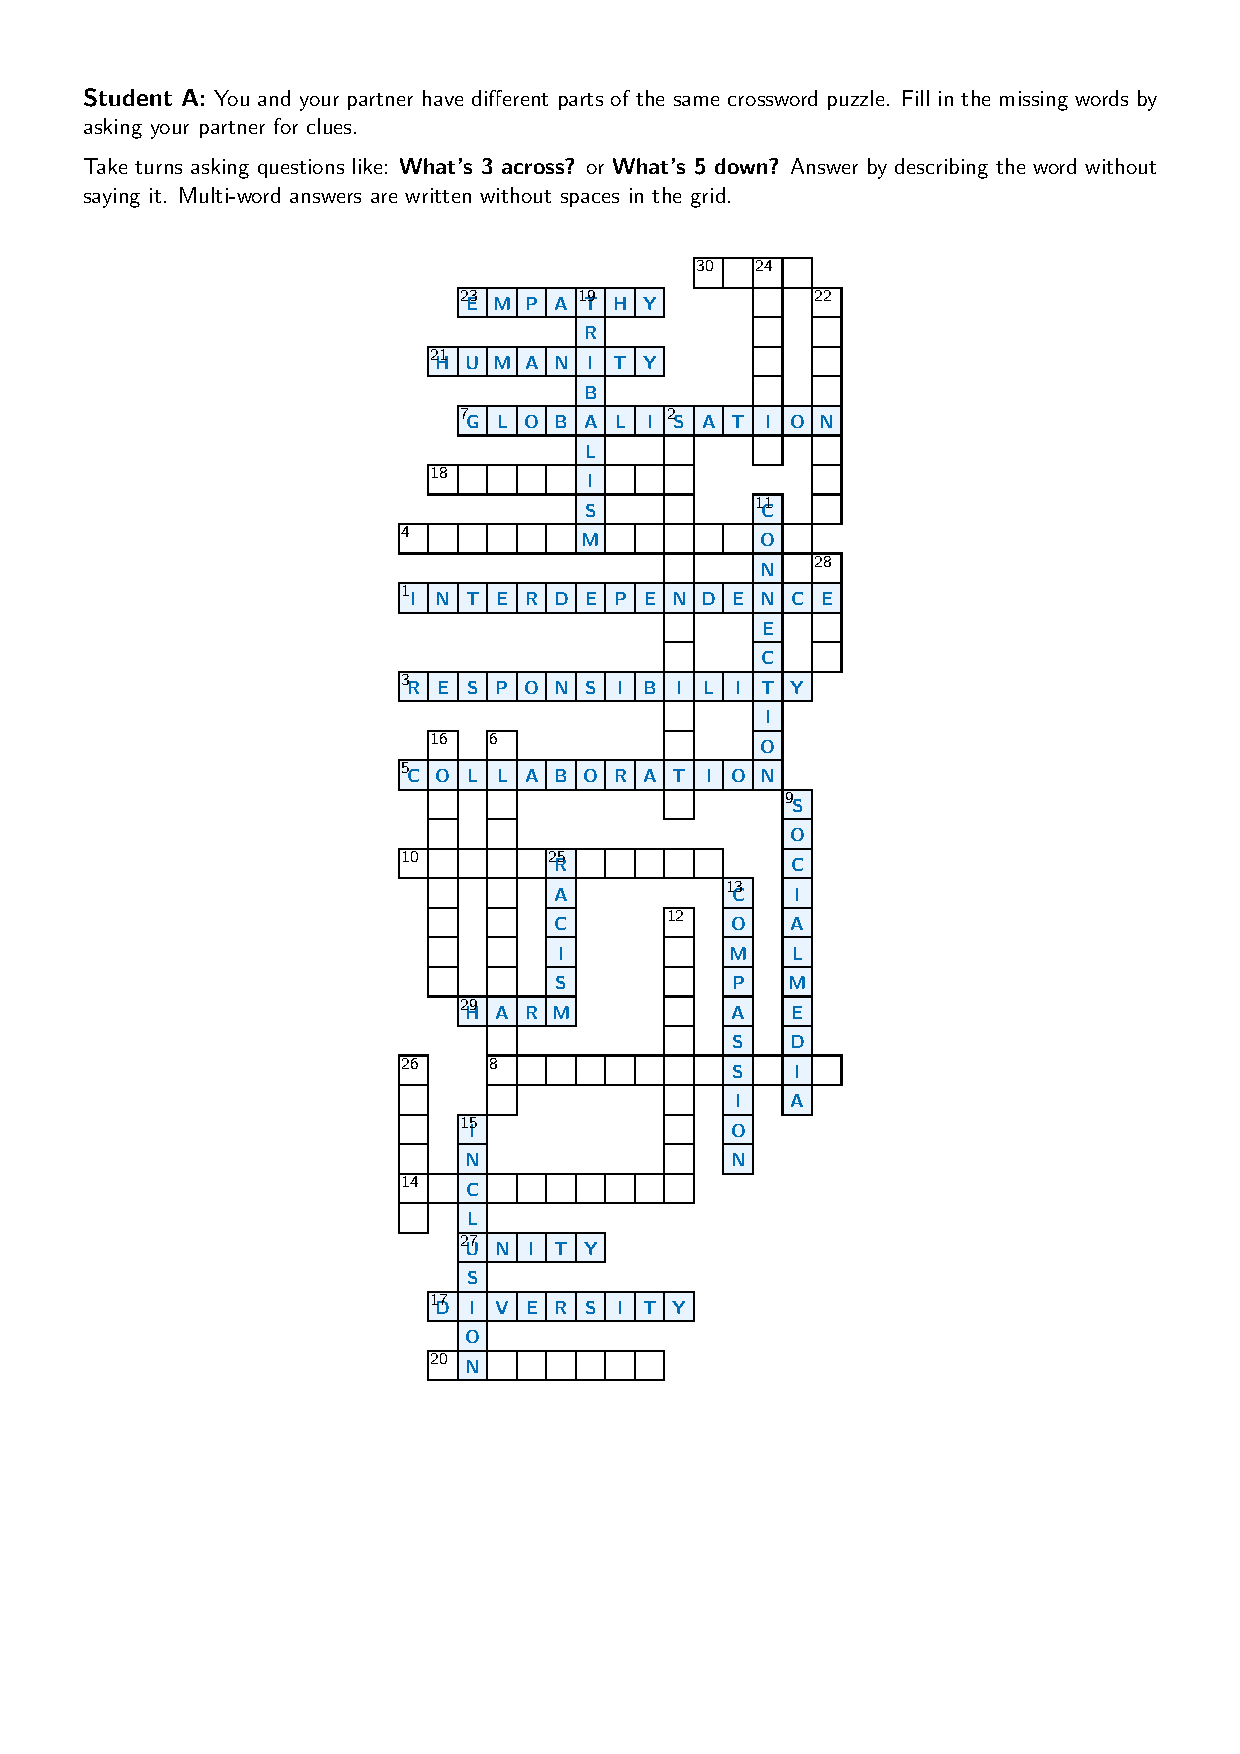
\includepdf[pages=-,scale=.9,pagecommand={\thispagestyle{fancy}},addtotoc={1,subsection,2,{voice half crossword},worksheet-13}]{materials/voice_half_crossword.pdf}

\clearpage\markboth{The Kings Speech Rhetorical Situation}{}
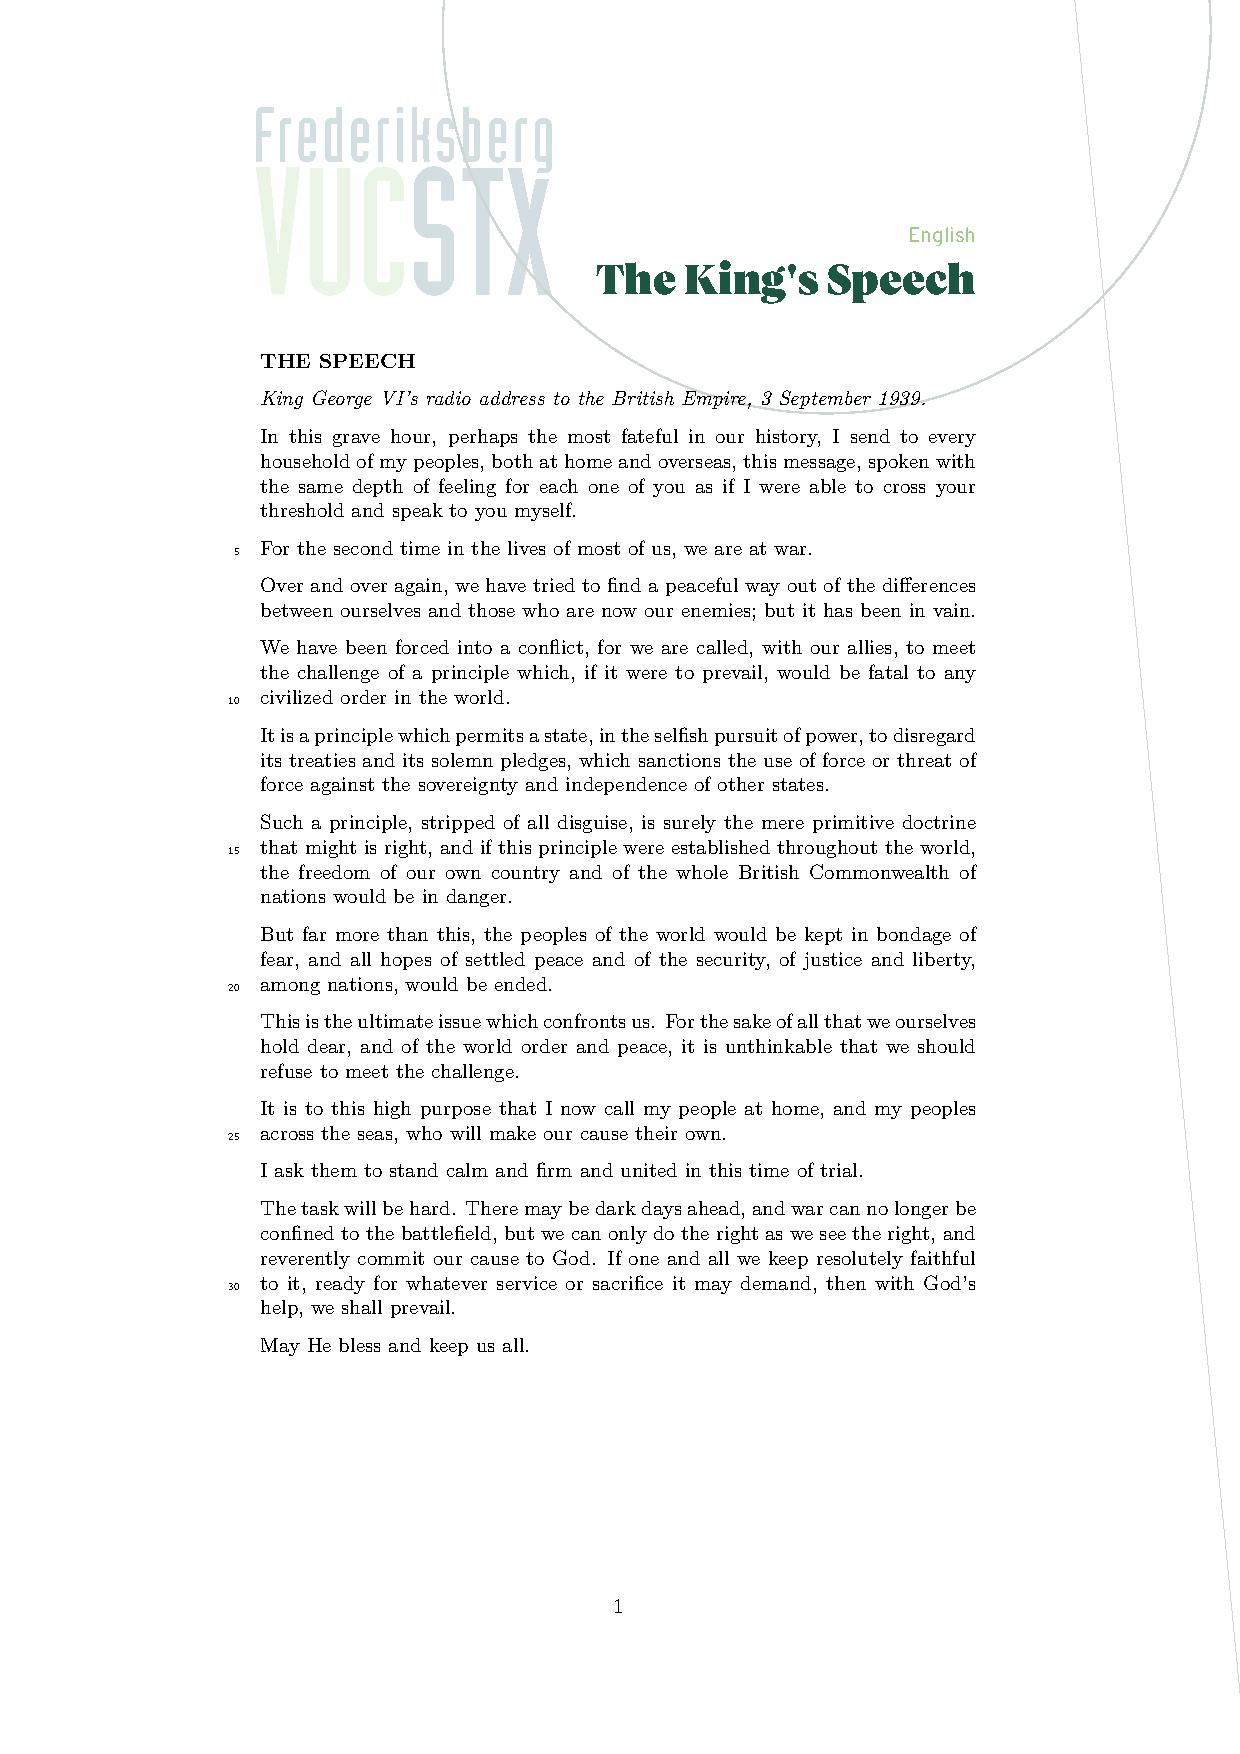
\includepdf[pages=-,scale=.9,pagecommand={\thispagestyle{fancy}},addtotoc={1,subsection,2,{The Kings Speech Rhetorical Situation},worksheet-14}]{materials/The_Kings_Speech_Rhetorical_Situation.pdf}

\clearpage\markboth{Brave New World — Worksheet}{}
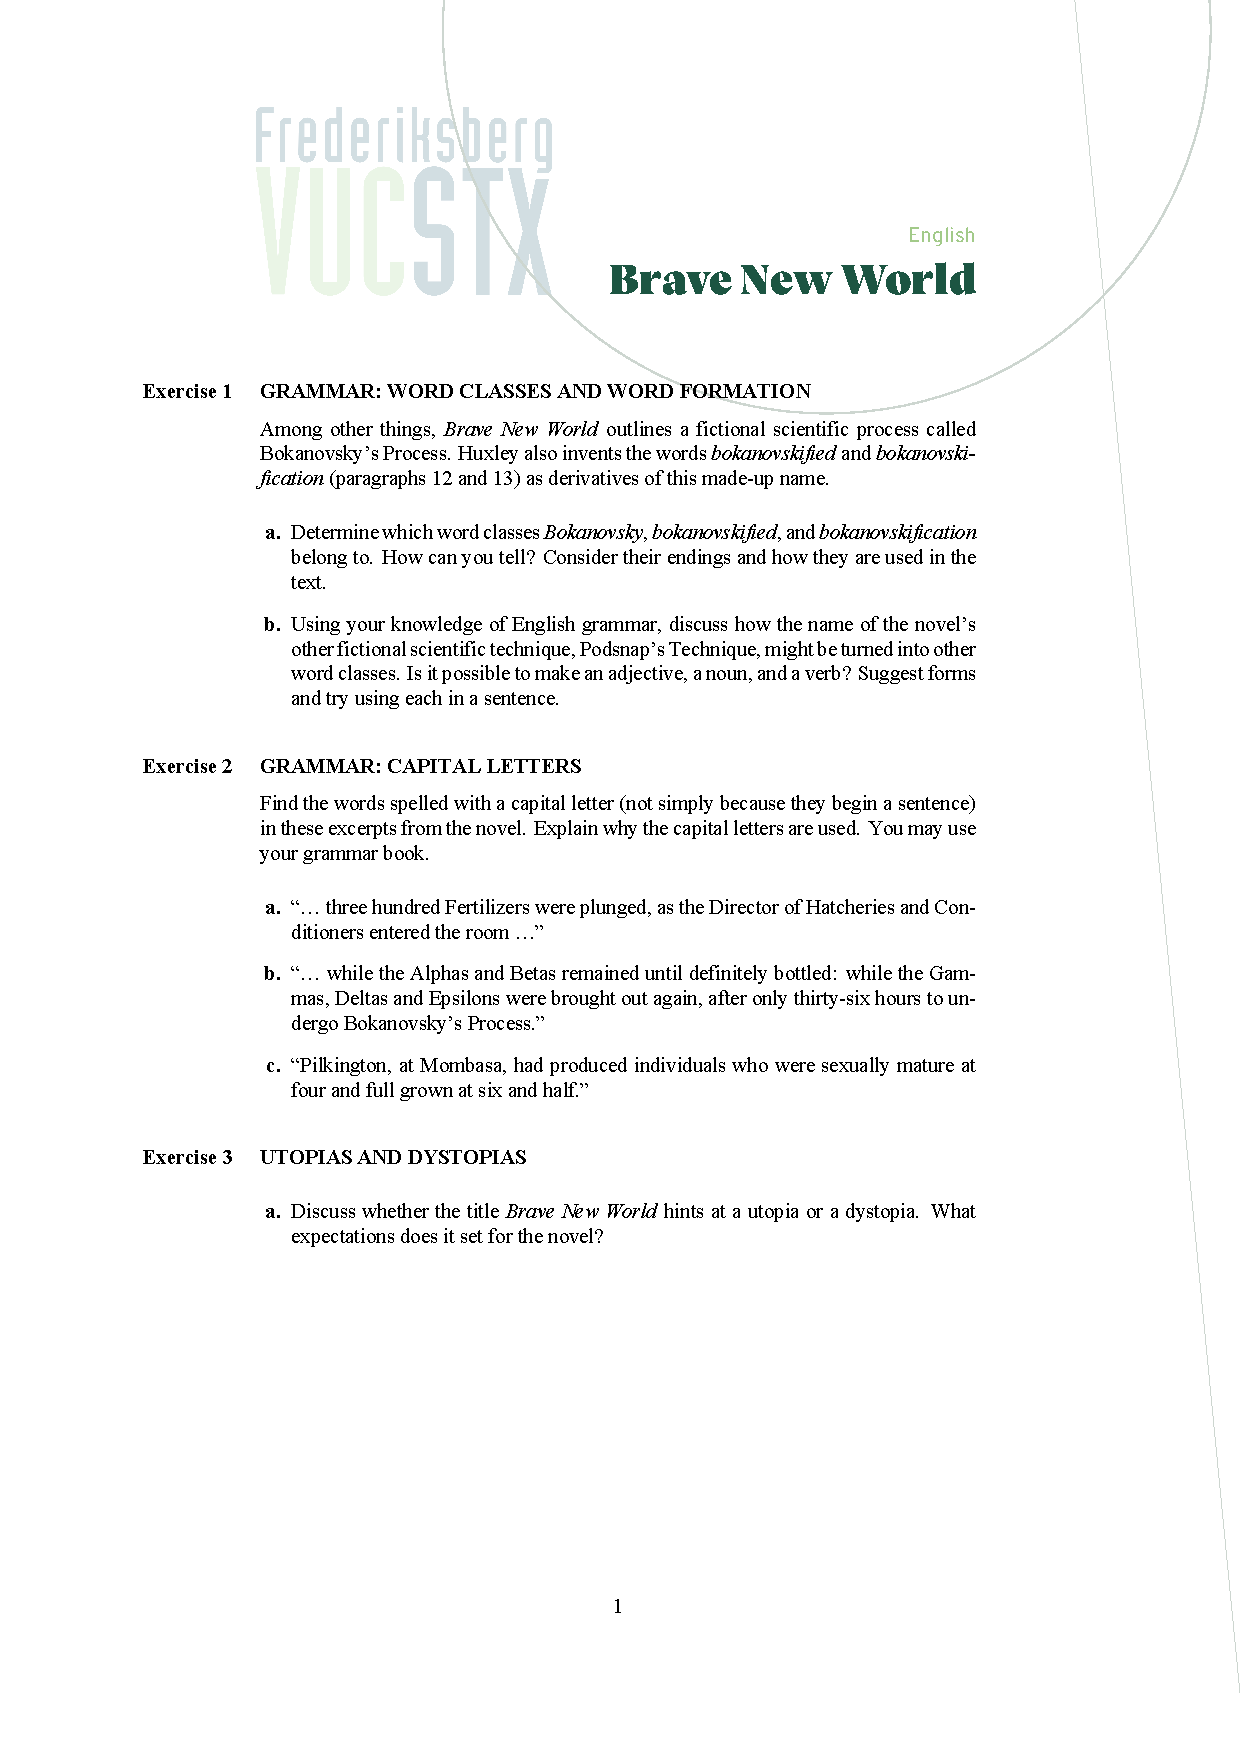
\includepdf[pages=-,scale=.9,pagecommand={\thispagestyle{fancy}},addtotoc={1,subsection,2,{Brave New World — Worksheet},worksheet-15}]{materials/Brave_New_World_Worksheet.pdf}

\clearpage\markboth{Brave New World II — Worksheet}{}
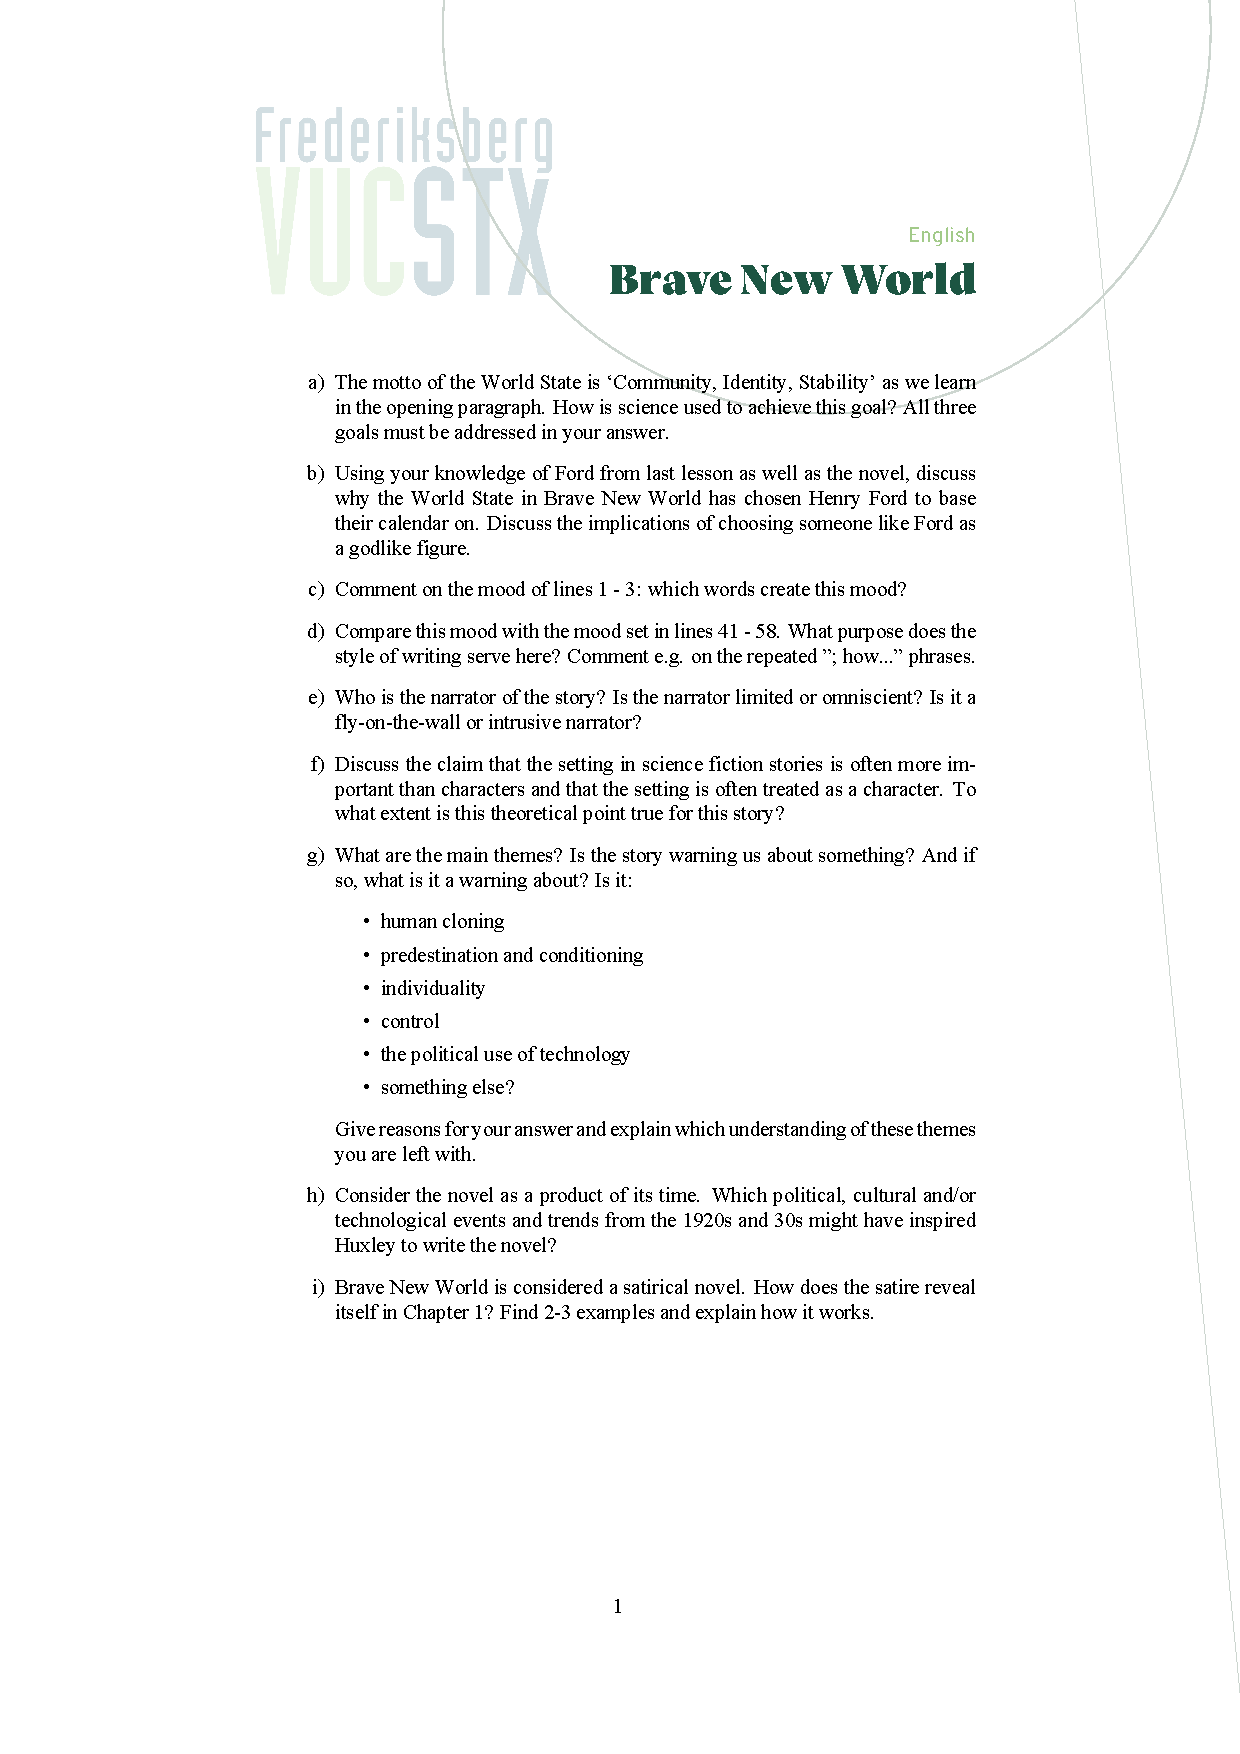
\includepdf[pages=-,scale=.9,pagecommand={\thispagestyle{fancy}},addtotoc={1,subsection,2,{Brave New World II — Worksheet},worksheet-16}]{materials/Brave_New_World_II_Worksheet.pdf}

\clearpage\markboth{The Relive Box — Worksheet}{}
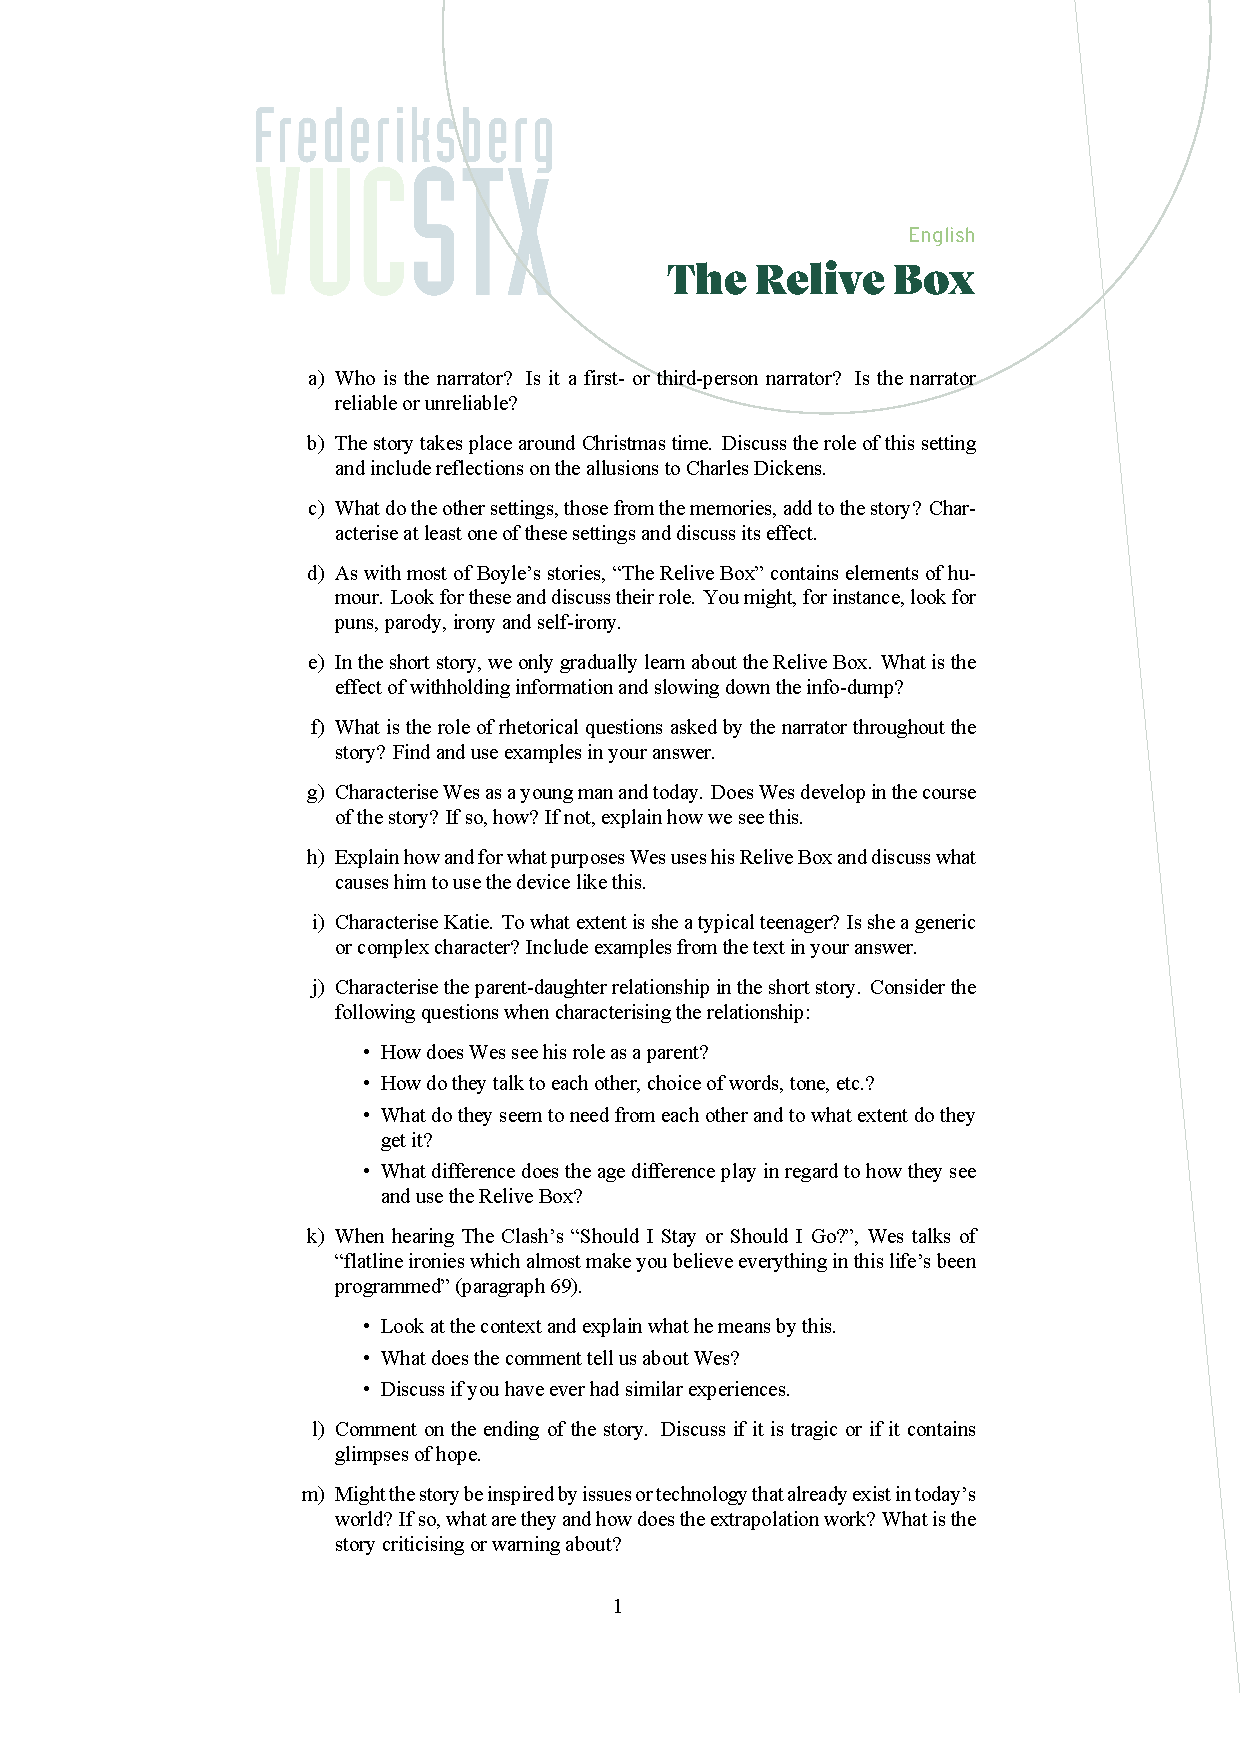
\includepdf[pages=-,scale=.9,pagecommand={\thispagestyle{fancy}},addtotoc={1,subsection,2,{The Relive Box — Worksheet},worksheet-17}]{materials/The_Relive_Box_Worksheet.pdf}

\clearpage\markboth{US Space Policy — Worksheet}{}
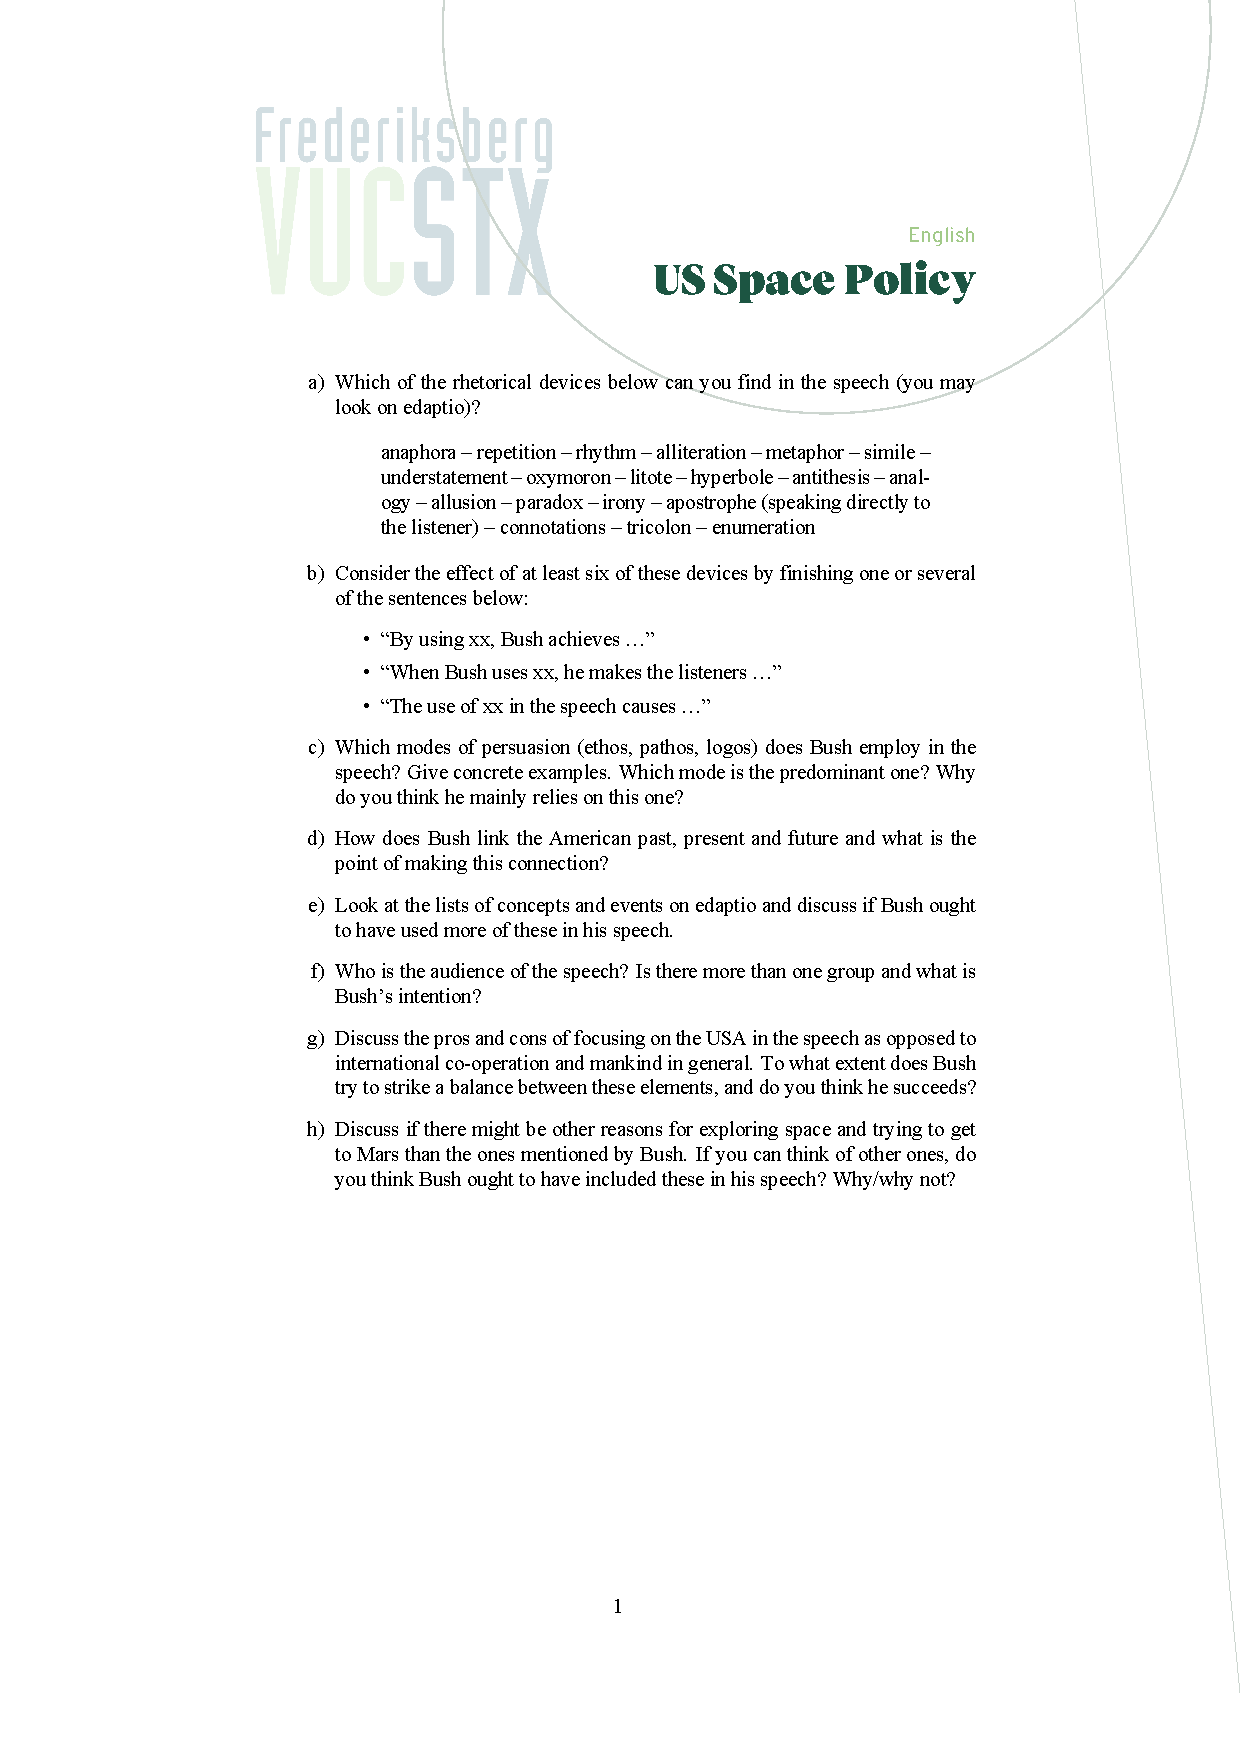
\includepdf[pages=-,scale=.9,pagecommand={\thispagestyle{fancy}},addtotoc={1,subsection,2,{US Space Policy — Worksheet},worksheet-18}]{materials/US_Space_Policy_Worksheet.pdf}

\clearpage\markboth{Settled In — Worksheet}{}
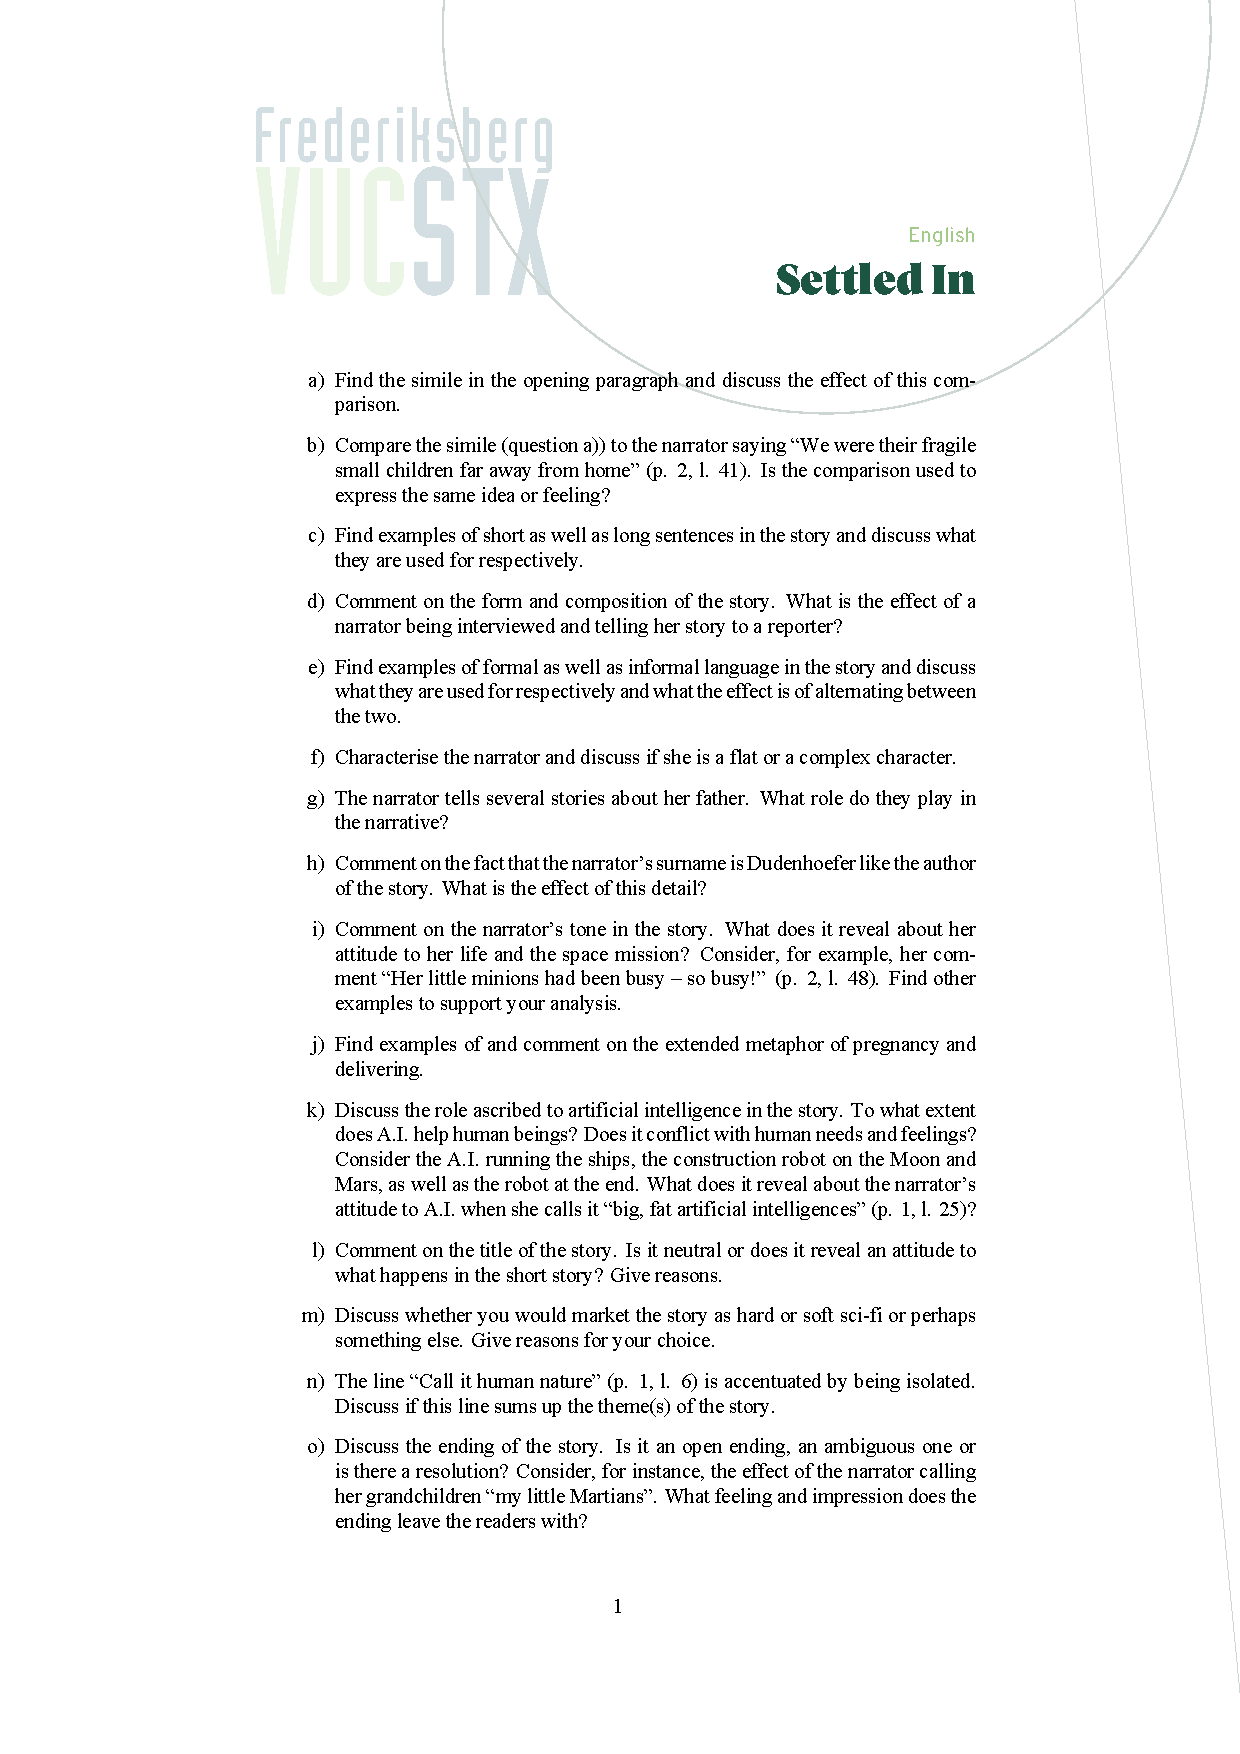
\includepdf[pages=-,scale=.9,pagecommand={\thispagestyle{fancy}},addtotoc={1,subsection,2,{Settled In — Worksheet},worksheet-19}]{materials/Settled_In_Worksheet.pdf}

\clearpage\fancyhead[L]{\small\color{blue}Notes}\markboth{Notes}{}\phantomsection\addcontentsline{toc}{chapter}{Notes}
{\displayfont\color{navy}\fontsize{30}{34}\selectfont Notes\par}\vspace{6mm}
Analysis guides and models. Click a title or page number to open a guide.\par
\begin{enumerate}
\item \hyperref[note-how-to-analyse]{How to analyse..} \hfill \hyperref[note-how-to-analyse]{p.~\pageref*{note-how-to-analyse}}
\item \hyperref[note-cinematic-techniques]{Cinematic techniques} \hfill \hyperref[note-cinematic-techniques]{p.~\pageref*{note-cinematic-techniques}}
\item \hyperref[note-flirt-model]{The FLIRT model} \hfill \hyperref[note-flirt-model]{p.~\pageref*{note-flirt-model}}
\item \hyperref[note-ace-model]{The ACE model} \hfill \hyperref[note-ace-model]{p.~\pageref*{note-ace-model}}
\item \hyperref[note-blooms-taxonomy]{Bloom's taxonomy} \hfill \hyperref[note-blooms-taxonomy]{p.~\pageref*{note-blooms-taxonomy}}
\item \hyperref[note-rhetorical-situation]{The rhetorical situation} \hfill \hyperref[note-rhetorical-situation]{p.~\pageref*{note-rhetorical-situation}}
\item \hyperref[note-rhetorical-devices]{Rhetorical devices} \hfill \hyperref[note-rhetorical-devices]{p.~\pageref*{note-rhetorical-devices}}
\item \hyperref[note-modes-of-appeal]{Modes of appeal} \hfill \hyperref[note-modes-of-appeal]{p.~\pageref*{note-modes-of-appeal}}
\end{enumerate}

\clearpage\phantomsection\label{note-how-to-analyse}\addcontentsline{toc}{section}{How to analyse..}\markboth{How to analyse..}{}
{\displayfont\color{navy}\fontsize{30}{34}\selectfont How to analyse..\par}\vspace{4mm}
Always support your points with examples from the text.


\section*{Fiction}

\subsection*{Setting}

\begin{enumerate}
\item Describe the physical setting.
\item Analyse the effect: Does the setting create a certain atmosphere? Does this influence the story / characters?
\end{enumerate}

\subsection*{Narrator}

\begin{enumerate}
\item Determine the type of narrator.
\item Analyse the effect: How does the narrator influence what we know about the characters and setting?
\end{enumerate}

\subsection*{Characterisation}

\begin{enumerate}
\item Describe how the main character(s) are presented.
\item Analyse their inner life and role in the story: What do we know about their values, personality, and relationships with the other characters? Do they develop?
\end{enumerate}

\subsection*{Theme}

\begin{enumerate}
\item Analyse the theme of the story: What does the story say about the theme? How is it visible in the story?
\end{enumerate}

\section*{Non-fiction}

\subsection*{Intention}

\begin{enumerate}
\item Describe the sender, audience, circumstances, language and subject of the text (the rhetorical pentagram).
\item Describe the \hyperref[note-rhetorical-situation]{rhetorical situation (p.~\pageref*{note-rhetorical-situation})} of the text:

\begin{itemize}
\item Determine the exigence: what change is the speaker hoping to achieve with the text?
\item Determine the constraints: What factors limit or influence the speaker's ability to persuade the audience?
\end{itemize}

\end{enumerate}

\subsection*{Method}

\begin{enumerate}
\item Analyse the structure of the text: How does it support the intention?
\item Analyse the \hyperref[note-modes-of-appeal]{modes of appeal (p.~\pageref*{note-modes-of-appeal})} (ethos, pathos and logos) used in the text:

\begin{itemize}
\item How credible is the writer/speaker, and how do they try to strengthen their credibility?
\item Does the writer/speaker try to make the audience be emotionally invested in the topic?
\item Does the writer/speaker try to convince the audience of something through logical arguments?
\item Are the modes of appeal used fitting for the context?
\end{itemize}

\item Describe the language of the text:

\begin{itemize}
\item Are \hyperref[note-rhetorical-devices]{rhetorical devices (p.~\pageref*{note-rhetorical-devices})} used, and to what effect?
\item How is the tone (inclusive, formal, informal, serious, humorous, ironic, sarcastic, optimistic, pessimistic, sympathetic, critical)?
\end{itemize}

\end{enumerate}

\subsection*{Execution}

\begin{enumerate}
\item Evaluate the effectiveness of the text:

\begin{itemize}
\item How well does method serve intention?
\item How well does the text respond to the rhetorical situation?
\end{itemize}

\end{enumerate}

\section*{Film and television}

\begin{enumerate}
\item Go through the steps in fiction or non-fiction above.
\item Analyse the use of \hyperref[note-cinematic-techniques]{cinematic techniques (p.~\pageref*{note-cinematic-techniques})}: How do they support e.g. characterisation, theme or intention?
\end{enumerate}

\section*{Graphic narratives}

\begin{enumerate}
\item Go through the steps in fiction or non-fiction above.
\item Analyse the relationship between words and images: How do dialogue, captions, sound effects and images complement or contradict each other, and how does this support e.g. characterisation, theme, or intention?
\end{enumerate}

\section*{Video games}

\begin{enumerate}
\item Go through the steps in fiction above.
\item Analyse the use of \hyperref[note-cinematic-techniques]{cinematic techniques (p.~\pageref*{note-cinematic-techniques})}, and the influence of game mechanics: How do they support e.g. characterisation or theme?
\end{enumerate}

\clearpage\phantomsection\label{note-cinematic-techniques}\addcontentsline{toc}{section}{Cinematic techniques}\markboth{Cinematic techniques}{}
{\displayfont\color{navy}\fontsize{30}{34}\selectfont Cinematic techniques\par}\vspace{4mm}

{\small\setlength{\tabcolsep}{4pt}\renewcommand{\arraystretch}{1.3}\begin{tabularx}{\linewidth}{@{}>{\raggedright\arraybackslash}X>{\raggedright\arraybackslash}X@{}}\toprule
Cinematic technique & Characteristics\\
\textbf{Framing} & \textbf{Close-up:} The character(s) are framed very closely.\newline{}\newline{}\textbf{Long shot:} Focus is on setting.\newline{}\newline{}\textbf{Medium shot:} Focus is on more than one character.\\
\textbf{Angles} & \textbf{Low angle:} The character in question seems powerful and big.\newline{}\newline{}\textbf{High angle:} The character in question seems small and maybe weak.\newline{}\newline{}\textbf{Eye level:} Audience at the same level as characters.\\
\textbf{Composition} & Foreground.\newline{}\newline{}Middle ground.\newline{}\newline{}Background.\\
\textbf{Sound} & \textbf{Diegetic sound:} Sound which is part of the film.\newline{}\newline{}\textbf{Non-diegetic sound:} Sound which is not part of the film.\newline{}\newline{}\textbf{Contrapuntal sound:} Sound in direct contrast to the images of the film.\\
\textbf{Lighting} & \textbf{Low key:} Difficult to see everything in the image.\newline{}\newline{}\textbf{High key:} Able to see everything in the image.\\
\textbf{Colour} & Each colour has both a positive and negative symbolism.\\
\bottomrule\end{tabularx}}\par\medskip

\clearpage\phantomsection\label{note-flirt-model}\addcontentsline{toc}{section}{The FLIRT model}\markboth{The FLIRT model}{}
{\displayfont\color{navy}\fontsize{30}{34}\selectfont The FLIRT model\par}\vspace{4mm}

\section*{F — Form}

\begin{itemize}
\item How is the poem structured into lines and stanzas? Does it follow a particular poetic form?
\item Are there changes, contrasts or developments in its structure?
\item How does the form support or contrast with the content?
\end{itemize}

\section*{L — Language}

\begin{itemize}
\item What kinds of words does the speaker use: formal, informal, emotional, concrete or abstract?
\item What tone do the word choices and sentence structures create?
\item Who is speaking, and who seems to be addressed? Do not automatically equate the speaker with the poet.
\end{itemize}

\section*{I — Imagery and rhetorical devices}

\begin{itemize}
\item Look for metaphors, similes, personification, symbols, allusion, antithesis, repetition, alliteration and onomatopoeia.
\item What images or associations do they create?
\item How do they support the poem's tone or ideas?
\end{itemize}

\section*{R — Rhyme / rhythm}

\begin{itemize}
\item Is there a rhyme scheme, or is the poem written in free verse?
\item What patterns of stress, repetition or pauses can you hear when reading it aloud?
\item Do sentences continue across line breaks (enjambment), or do they pause at the end of lines?
\item How do these choices affect pace, emphasis and meaning?
\end{itemize}

\section*{T — Theme}

\begin{itemize}
\item What central ideas or conflicts does the poem explore?
\item What does it suggest about these ideas? A topic might be \emph{identity}; an interpretation of its theme explains what the poem says about identity.
\item How do form, language, imagery and rhythm support your interpretation?
\end{itemize}

\clearpage\phantomsection\label{note-ace-model}\addcontentsline{toc}{section}{The ACE model}\markboth{The ACE model}{}
{\displayfont\color{navy}\fontsize{30}{34}\selectfont The ACE model\par}\vspace{4mm}

\section*{A — Answer}
Answer the question with a clear analytical point. If there is no set question, make a claim about the text.


\section*{C — Cite}
Support your answer with specific evidence: a short quotation, a precise reference to an event, or a description of an image or scene. Give line numbers, page numbers or a timestamp where available. Integrate quotations into your own sentences.


\section*{E — Explain}
Explain how the evidence supports your answer. Analyse significant words, details or techniques and their effect. Connect them to characterisation, atmosphere, theme or intention where relevant.

Do not simply repeat the quotation in different words or assume that it speaks for itself.


\clearpage\phantomsection\label{note-blooms-taxonomy}\addcontentsline{toc}{section}{Bloom's taxonomy}\markboth{Bloom's taxonomy}{}
{\displayfont\color{navy}\fontsize{30}{34}\selectfont Bloom's taxonomy\par}\vspace{4mm}

{\small\setlength{\tabcolsep}{4pt}\renewcommand{\arraystretch}{1.3}\begin{tabularx}{\linewidth}{@{}>{\raggedright\arraybackslash}X>{\raggedright\arraybackslash}X>{\raggedright\arraybackslash}X@{}}\toprule
Level & What you do & Example question or task about \emph{Severance}\\
\textbf{Remember} & Recall facts and identify details. & What happens when Helly wakes up at the table?\\
\textbf{Understand} & Explain meaning in your own words. & Explain how the severance procedure affects memory.\\
\textbf{Apply} & Use a concept or method in a particular situation. & Use the concept of private and public identity to explain Mark's two lives.\\
\textbf{Analyse} & Examine parts, patterns and relationships; explain how something works. & How do framing and lighting create a contrast between life inside and outside Lumon?\\
\textbf{Evaluate} & Make a judgement using evidence and clear criteria. & Does the procedure allow meaningful consent? Judge it using what the characters know and their ability to withdraw.\\
\textbf{Create} & Combine ideas into something new. & Write a scene in which an innie communicates with their outie, using details from the episode.\\
\bottomrule\end{tabularx}}\par\medskip

\clearpage\phantomsection\label{note-rhetorical-situation}\addcontentsline{toc}{section}{The rhetorical situation}\markboth{The rhetorical situation}{}
{\displayfont\color{navy}\fontsize{30}{34}\selectfont The rhetorical situation\par}\vspace{4mm}

\begin{itemize}
\item \emph{Exigence} What is the (real) purpose of the text? What is the speaker/writer trying to achieve/change? A situation becomes rhetorical once you believe that you can change something in life by uttering something.
\item \emph{Audience} Who is the text meant for? What is the medium, and who is the specific audience of this medium? What is their social background, political and religious belief, age, nationality, gender, ethnicity, etc.? The will be the \emph{mediators of change} who can act on the exigence (i.e. do something about the issue).
\item \emph{Constraints} The rhetorical situation will have som limitations and possibilities related to the context, the speaker/writer, and the mediators of change. These are the constraints. To make a change as likely as possible, what can then be said? What can not?
\end{itemize}

\clearpage\phantomsection\label{note-rhetorical-devices}\addcontentsline{toc}{section}{Rhetorical devices}\markboth{Rhetorical devices}{}
{\displayfont\color{navy}\fontsize{30}{34}\selectfont Rhetorical devices\par}\vspace{4mm}

\section*{Devices}

\begin{itemize}
\item alliteˈration: the repetition of a consonant sound at the beginning of words which are close together
\item aˈnaphora: the repetition of one or more words at the beginning of successive clauses
\item anˈtithesis: the placing together of opposing words or ideas to show a contrast
\item ˈassonance: the repetition of vowel sounds in words which are close together
\item ˈmetaphor: an image described by a word or phrase with a concrete meaning but used figuratively
\item personifiˈcation: language in which an inanimate object or concept is spoken of as if it had human life
\item repetition
\item ˈsimile: a figure of speech in which two unlike things are compared using ‘like’ or ‘as’
\item the list of three: three things are listed immediately after each other.
\item inclusive language: language that addresses or includes the audience, often using pronouns such as ‘we’, ‘us’, and ‘our’
\end{itemize}

\clearpage\phantomsection\label{note-modes-of-appeal}\addcontentsline{toc}{section}{Modes of appeal}\markboth{Modes of appeal}{}
{\displayfont\color{navy}\fontsize{30}{34}\selectfont Modes of appeal\par}\vspace{4mm}

\begin{itemize}
\item pathos: an appeal to the audience’s emotions using emotional language, passion and a personal angle
\item logos: an appeal to reason with arguments, evidence, facts and logical reasoning
\item ethos: an appeal to the audience’s trust by sounding eloquent, or by establishing authority or expertise on the subject.
\end{itemize}
\textbf{Example} "Trump uses antithesis when he says that America rejects globalism and embraces patriotism. This device is used to make a pathos appeal to patriotic feelings, which targets American voters and citizens, who can mediate political change by supporting his nationalist policies and voting for leaders who put America first."


\end{document}
